\documentclass{article}
\usepackage{graphicx}
\usepackage{pdfpages}
\usepackage[utf8]{inputenc}                                      
\usepackage{csquotes}
\usepackage[T1]{fontenc} 
\usepackage{amsmath,amsfonts,amssymb,amsthm}
\usepackage{graphicx} 
\usepackage{hyperref}
\usepackage[page]{appendix} 
\usepackage{booktabs}
\usepackage{hyperref}
\usepackage[backend=bibtex,maxcitenames=10,mincitenames=2]{biblatex}
\usepackage{indentfirst}
\usepackage{setspace}
\usepackage{float}
\usepackage{listings}
\usepackage{stackengine}
\usepackage{multirow}
\usepackage{multicol}
\usepackage{array}
\usepackage{wasysym}
\usepackage[polish]{babel}

\newcommand\xrowht[2][0]{\addstackgap[.5\dimexpr#2\relax]{\vphantom{#1}}}

\onehalfspacing{}

\usepackage[polish]{babel} 
\usepackage{lmodern}
\usepackage{graphicx} 
\usepackage{booktabs}
\frenchspacing
\tolerance= 1
\emergencystretch=\maxdimen{}

\nocite{*}
\addbibresource{bibliography}


% \fancypagestyle{phdthesis}{
% \fancyhead[C]{\thepage}
% }

\lstset{%
    % language=Python,
    % commentstyle=\textit,
    % identifierstyle=\textsf,
    % keywordstyle=\sffamily\bfseries,
    % %captionpos=b,
    % tabsize=3,
    % frame=lines,
    numbers=left,
    numberstyle=\tiny,
    % numbersep=5pt,
    % breaklines=true,
    % morekeywords={descriptor_gaussian,descriptor,partition,fcm_possibilistic,dataset,my_exception,exception,std,vector},
    escapeinside={@*}{*@},
    %texcl=true,
}

\colorlet{punct}{red!60!black}
\definecolor{background}{HTML}{EEEEEE}
\definecolor{delim}{RGB}{20,105,176}
\colorlet{numb}{magenta!60!black}
\lstdefinelanguage{json}{
    basicstyle=\normalfont\ttfamily,
    numbers=left,
    numberstyle=\scriptsize,
    stepnumber=1,
    numbersep=8pt,
    showstringspaces=false,
    breaklines=true,
    frame=lines,
    % backgroundcolor=\color{background},
    literate=
     *{0}{{{\color{numb}0}}}{1}
      {1}{{{\color{numb}1}}}{1}
      {2}{{{\color{numb}2}}}{1}
      {3}{{{\color{numb}3}}}{1}
      {4}{{{\color{numb}4}}}{1}
      {5}{{{\color{numb}5}}}{1}
      {6}{{{\color{numb}6}}}{1}
      {7}{{{\color{numb}7}}}{1}
      {8}{{{\color{numb}8}}}{1}
      {9}{{{\color{numb}9}}}{1}
      {:}{{{\color{punct}{:}}}}{1}
      {,}{{{\color{punct}{,}}}}{1}
      {\{}{{{\color{delim}{\{}}}}{1}
      {\}}{{{\color{delim}{\}}}}}{1}
      {[}{{{\color{delim}{[}}}}{1}
      {]}{{{\color{delim}{]}}}}{1},
}

\hyphenpenalty= 100000
\widowpenalty= 100000
\clubpenalty= 100000

\begin{document}

% \justifying

\begin{titlepage}
    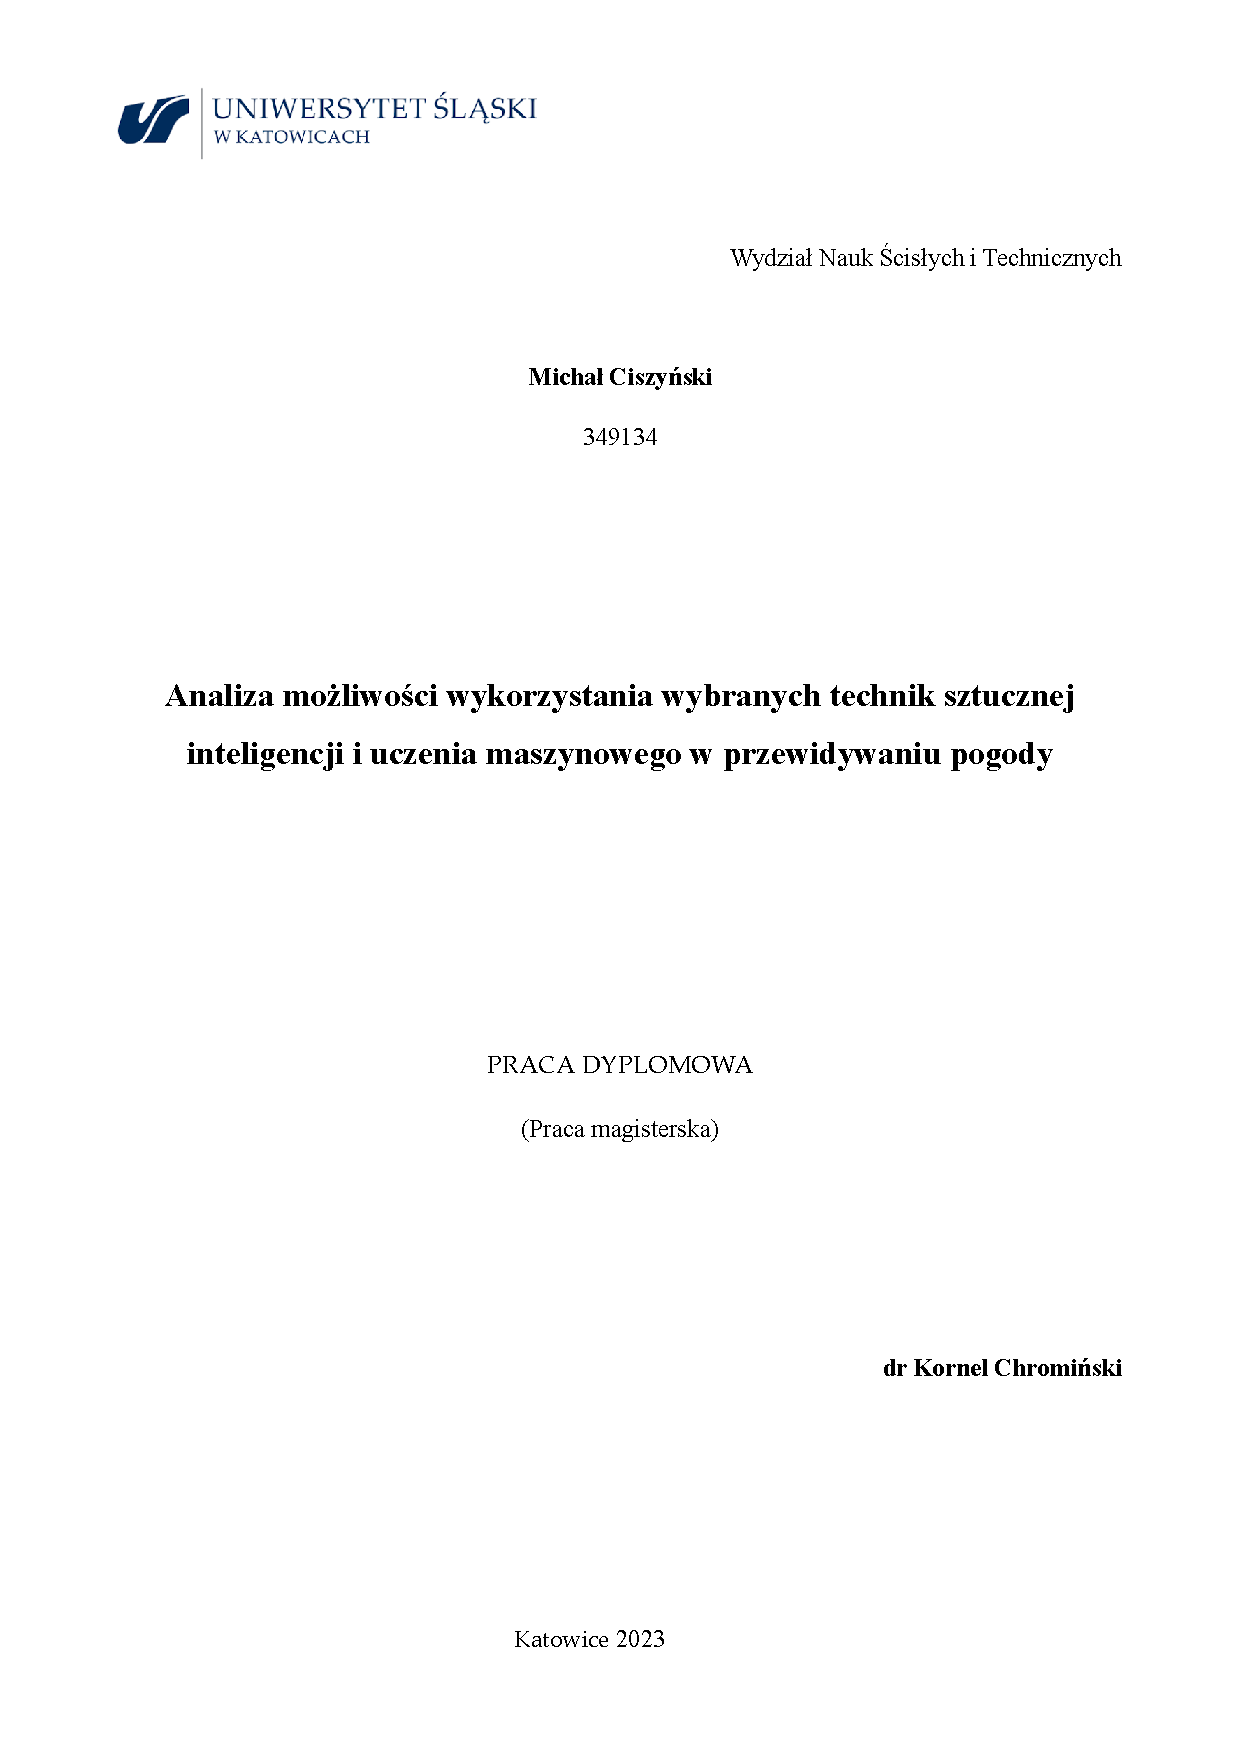
\includepdf{titlepage.pdf}
\end{titlepage}

\tableofcontents
\pagebreak

\section*{Abstrakt}

Niniejsza praca zajmuję się analizą wykorzystania uczenia maszynowego w~zastosowaniach meteorologicznych
w problemie prognozowania pogody. W~celu pokazania działania poszczególnych modeli wykorzystany został
zbiór danych ERA5 stworzony przez Europejskie Centrum Średnioterminowych Prognoz Pogody zawierający
dane globalne zasymilowane przez najnowsze modele numeryczne. W celach tej pracy analiza skupiała 
się na krótkoterminowym prognozowaniu pogody w zakresie 24 godzin,
a zakres geograficzny analizowanych danych skupiał się na jednej lokalizacji. 
Stworzone modele zostały poddane wstępnej optymalizacji poprzez dostrajanie wartości hiperparametrów.

Wśród rozważonych modeli znajdowały się SVR, regresja logistyczna, regresja SGD,
k najbliższych sąsiadów, regresja gaussowska, drzewo decyzyjne, las losowy, sieci neuronowe,
oraz regresja dekompozycji PLS.

Wśród rozpatrzonych metryk znajdował się błąd średniokwadratowy, średni błąd absolutny oraz współczynnik
korelacji. Dodatkowo rozpatrzone zostały parametry statystyczne wytworzonych prognoz w porównaniu
do danych rzeczywistych. Wskutek przeprowadzonych badań stworzone zostało wszechstronne porównanie
analizowanych modeli względem siebie, a~przeprowadzone wnioskowanie poddało analizie 
mocne i słabe strony poszczególnych podejść.

Dodatkowy nacisk został położony w analizie metod uczenia maszynowego w~zastosowaniu razem z 
tradycyjnymi metodami numerycznymi symulacji pogody. 

\bigskip

\noindent
{\bf Słowa kluczowe:} Uczenie maszynowe, Uczenie Głębokie, Sieci neuronowe,
ERA5, Prognozowanie pogody, Sztuczna inteligencja
\pagebreak

% Provide an overview of the topic, 
% motivation for the research, and the scope of the study.

% The introduction to your thesis is an essential 
% part of your work, as it provides the reader with an 
% overview of your research, its significance, and its objectives. 
% Here are some important elements to consider including in your introduction:

% Background and context: Begin by providing some background 
% information on the topic of weather prediction and the application 
% of artificial intelligence and machine learning techniques in this area. 
% This could include a brief overview of the current state of the field, the 
% challenges that exist, and the potential benefits of using these techniques.

% Problem statement: Clearly articulate the research problem you are 
% addressing, and explain why it is important. This could involve discussing 
% the limitations of current weather prediction methods, or the potential 
% benefits of improving the accuracy and reliability of these predictions.

% Research objectives: Clearly state the objectives of your research, 
% including any hypotheses you are testing or research questions you 
% are exploring. This helps the reader understand the scope and focus of your work.

% Research methods: Provide an overview of the research methods you have used, 
% including the data sources you have used, the models you have developed, 
% and the evaluation metrics you have used to measure performance.

% Contribution to the field: Conclude by discussing the contribution 
% of your research to the field of weather prediction and the broader 
% field of artificial intelligence and machine learning. This could 
% include highlighting the novelty of your approach, the potential 
% impact of your findings, or the implications for future research.

% Overall, your introduction should provide the reader with a clear 
% understanding of the research problem you are addressing, the methods 
% you have used to explore this problem, and the significance of your 
% findings. It should also engage the reader and motivate them to read 
% on, by highlighting the importance and relevance of your research.

% "The results of this research demonstrate that the application 
% of artificial intelligence and machine learning techniques in 
% weather prediction is a promising approach, as the results 
% obtained are comparable to those achieved by established techniques in the field."

% In this thesis statement, you highlight the contribution 
% of your research in showing the promise of artificial 
% intelligence and machine learning techniques in weather 
% prediction. You also emphasize that your results are 
% comparable to those obtained by other approaches, which 
% underscores the reliability and validity of your research findings.
\section{Wstęp}
% Conduct a comprehensive review of the existing literature 
% on artificial intelligence and machine learning techniques 
% used in weather prediction. Discuss the strengths and limitations 
% of these approaches

% The literature review section of your thesis is a critical component 
% of your research, as it provides a comprehensive overview of the 
% current state of knowledge on the topic of weather prediction and 
% the application of artificial intelligence and machine learning 
% techniques in this area. Here are some important elements to consider 
% including in your literature review:

% Overall, your literature review should provide a comprehensive overview of 
% the existing literature on weather prediction and the application of artificial 
% intelligence and machine learning techniques in this area. It should also 
% highlight the importance of your research question, and explain how your research 
% contributes to the broader understanding of the field.
\section{Przegląd literatury}

Jako już dojrzała metodologia, zastosowanie uczenia maszynowego 
znajduje dużą duże odbicie w wielu artykułach i publikacjach naukowych. 
Wiele publikacji analizuje zastosowanie AI w hybrydowych, jak i czystych 
algorytmach prognozowania pogody. 


% Background information: Begin by providing some background information on 
% the topic of weather prediction and the challenges that exist in this area. 
% This could include discussing the impact of weather on human life and the 
% economy, the limitations of current weather prediction methods, and the potential 
% benefits of using artificial intelligence and machine learning techniques to 
% improve accuracy.
\subsection{Tło teoretyczne}


\subsubsection{Metody NWP}

Pierwsze próby "odręcznych" modeli NWP były zainicjowane przez Lewis Fry Richardson-a w 1922 roku i 
były zainspirowane ideą przewidywania pogody za pomocą sformułowanych praw fizyki. Sformułowanie
nieliniowych równań różniczkowych opisujących pogodę tworzyło problem z wartością początkową bazującą
na bieżących pomiarach pogody. W celu osiągnięcia zamierzonego celu interakcje z dziedziny 
termodynamiki, dynamiki, procesów chemicznych, jak i biologicznych muszą być wzięte pod uwagę.
Pierwsze komputerowo wspomagane prognozy pogody były tworzone już w 1950 roku, lecz dopiero
w 1970 roku wraz z rozwojem superkomputerów rozwiązanie pełnego zbioru równań było możliwe.

Podstawowymi równaniami opisującymi zachowanie pogody są równania Naviera-Stokesa, równania zachowania
masy, pierwsza zasada termodynamiki i równanie Clapeyrona. Za pomocą nich stan wiatru, ciśnienia,
gęstości, temperatury może być modelowany opisując stan atmosfery. Ze względu na brak rozwiązania
analitycznego tych równań, koniecznością jest rozwiązanie numeryczne. Procesy fizyczne występujące
w zbyt małej skali, aby być ujęte podczas dyskretyzacji przestrzeni, muszą być opisywane za pomocą
parametryzacji próbujących przybliżyć ich wpływ na ogólne rozwiązanie. W wielu przypadkach 
dodatkowe uproszczenia i zaokrąglenia są brane pod uwagę w celu uproszczenia procesu
rozwiązywania. Niektóre modele globalne i prawie wszystkie modele lokalne stosują 
metodę różnic skończonych we wszystkich stopniach swobody systemu, a niektóre modele globalne
wykorzystują metodę różnic skończonych w kierunku pionowym a metody spektralne w kierunku równoległym
do powierzchni ziemi. Krok czasu stosowany w stosunku do modeli globalnych jest wielkości dziesiątek
minut, a w przypadku prognoz lokalnych w zakresie jednej do czterech minut.

Ze względu na chaotyczną charakterystykę równań opisujących pogodę, małe zmiany w warunkach początkowych
mogą skutkować odstającymi od siebie wynikami. W celu opisania i przewidywania błędu prognozy pogody 
rozwinięte zostały modele ensemble. Nieliniowa złożoność systemu oznacza, że podejścia opisu
dokładności prognozy bazujące na metodach czysto statystycznych nie przynoszą upragnionych wyników.
Dlatego zbiór wielu modeli zainicjowanych z nieznacznie różniącymi się warunkami początkowymi
jest stosowany do sprawdzenia jak bardzo uzyskane wyniki mogą się różnić, i nadania dokładności do 
stworzonej prognozy. Przykładowa predykcja stworzona przy pomocy metody ensemble znajduje się 
poniżej\ref{nwp-ensemble}.

\begin{figure}[H]
    \centering
    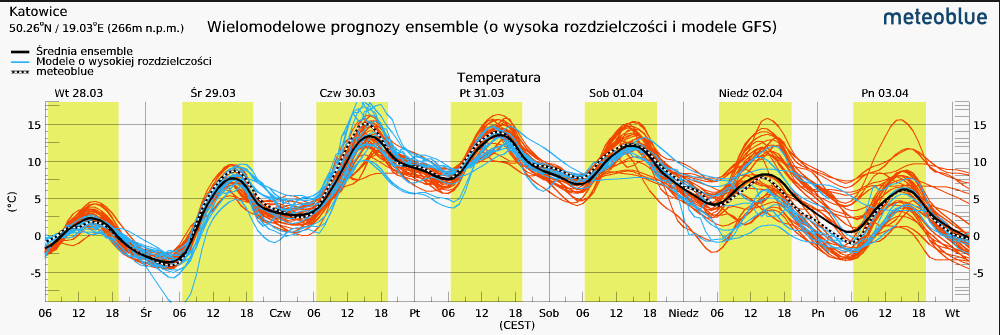
\includegraphics[width=\textwidth]{images/multimodel.png}
    \caption{Przykładowy wynik działania modelu ensemble pochodzący ze strony 
        \url{https://www.meteoblue.com/pl/pogoda/prognoza/multimodel/katowice_polska_3096472}}
    \label{nwp-ensemble}
\end{figure}

Wczesne metody specyfikacji warunków początkowych opierały się na analizie graficznych wykresów 
pogodowych. Następnie różne metody interpolacji danych były zastąpione przez algorytmy
asymilacji danych oparte na teorii sterowania optymalnego. Obliczanie rzeczywistych wartości
opisujących atmosferę może być opisane jako wnioskowane Bayesowskie oparte na wynikach pomiarów
oraz ich niepewnościach. Te obliczenia skoncentrowane na minimalizacji obiektywnej funkcji 
są przeprowadzane w czterowymiarowej przestrzeni, aby otrzymać fizycznie możliwy wynik
równomiernie rozłożony w trzech wymiarach przestrzennych i czasie.

W praktyce wykorzystanie modeli NWP w celach predykcji pogody wymaga asymilacji dużej ilości
danych pochodzących z różnych źródeł. Metodą wykorzystywaną dzisiaj w celu wprowadzenia
danych jest asymilacja 4D-Var (używana od 1980 roku). W tym algorytmie dla każdego typu obserwacji tworzony jest
operator obserwacji pozwalający wewnętrznym parametrom modelu NWP na odniesienie się
do poszczególnego typu obserwacji. Podczas procesu asymilacji danych parametry wewnętrzne
modelu są dostosowywane, aby jak najlepiej odzwierciedlić rzeczywiste warunki pogodowe.

W wielu przypadkach złożoność obliczeniowa NWP wymaga redukcji objętości danych pochodzących
z obserwacji satelitarnych o dużej gęstości. Rozdzielczość danych pochodzących z odczytów
satelitarnych znacznie przekracza możliwości dotychczas używanych modeli stworzonych przez
ECMWF posiadających rozdzielczość horyzontalną równą 9 km. Co więcej, w przypadku modeli
ensemble w celach zmniejszenia kosztów obliczeniowych rozdzielczość jest zmniejszana do 18 km.
Procesy, które nie mogą być wiernie odzwierciedlone przez symulację
ze względu na zbyt małą rozdzielczość NWP podlegają parametryzacji.
Do takich procesów zalicza się: formowanie się chmur, ilość promieni słonecznych docierających do 
podłoża, opór aerodynamiczny szczytów górskich czy formowanie się kropelek wody.

Ostateczny wynik przeprowadzonej symulacji NWP musi być jeszcze dodatkowo wzbogacony przez zastosowanie
statystyk wyjścia modelu (MOS). W ramach tego prognozowany stan modelu opisywany poprzez skomplikowane
parametry jest zamieniany na wielkości łatwo interpretowane przez ludzi. Co więcej, metody numeryczne
wykorzystują przybliżoną siatkę modelującą atmosferę, która musi być interpolowana w celu uzyskania
wyniku dla konkretnej lokalizacji. W tych celach często stosuje się wielokrotne zastosowanie 
regresji liniowej. Krok ten dodatkowo umożliwia zniwelowanie błędów nawarstwionych przez model i wzięcie
pod uwagę sparametryzowanych zjawisk.

Dodatkowo niektóre parametryzacje także są stopniowo zastępowane przez algorytmy uczenia maszynowego,
czego przykładem jest obliczanie energii promieniowania w sposób uproszczony
\cite{ai-in-weather-and-climate-prediction}. Energia promieniowania
może być w sposób kosztowny obliczona przez modele NWP, lecz zastosowanie ML skutkuje szybszym
procesem prognozowania.

Przykładowymi modelami prognozowania pogody są Lorenz63 i Lorenz96\cite{ai-in-weather-and-climate-prediction}
które są najprostsze w opisie,
które są zaprojektowane z mniejszą ilością stopni swobody. Modele te są łatwe w zrozumieniu i 
stanowią podstawe do przeprowadzania badań. Ich szybka natura sprawia, że ich stosowanie jest dość
proste, niestety dokładność predykcji jest dość niska. Przeciwieństwem do nich są modele NWP i GCM,
które są bardzo skomplikowane i trudne do zrozumienia, są opisane przez wielowymiarowe równania, oraz
osiągają większą dokładność.

Jednym z większych problemów NWP jest nieliniowo wzrastający błąd ograniczający długość prognozy.
Ponieważ modele NWP dokonują predykcji w sposób stopniowy, prognozując stan systemu dla następnego
kroku, żeby później otrzymany wynik dodać do danych wejściowych i kontynuować obliczenia, otrzymane błędy
mają tendencję do akumulacji wraz ze wzrostem długości symulacji.
Limit dla wydarzeń o małej skali jest szacowany na dni bądź godziny, zdarzenia o dużej skali
mogą być prognozowane z aż 2 tygodniowym wyprzedzeniem. Szacuje się że błąd akumulowany przez 
model NWP ulega zdwukrotnieniu z każdymi pięcioma dniami.

W porównaniu z wieloma innymi dziedzinami, w których numeryczne prognozowanie jest stosowane,
NWP ma przewagę pod względem częstotliwości, z którą jest wykorzystywane. Prognozy są generowane
w ten sposób z częstotliwością dzienną i na poziomie globalnym. Dokładność tworzonych predykcji jest
dobrze znana i sposoby wzmocnienia aktualnie stosowanych algorytmów mogą być sprawdzone z dużą
efektywnością. Modele NWP wciąż są ulepszane, a rozwój technologiczny i naukowy być może pozwoli
w przyszłości tworzyć modele bazujące na danych zbieranych z rozdzielczością sięgającą 1 km. Co więcej
możliwe, że w najbliższej przyszłości utworzone zostaną modele rozwiązujące sprzężone symulacje
dla atmosfery, lądu oraz oceanu\cite{nwp-the-quiet-revolution}.

Dzisiejsze komputery używane do NWP sięgają mocy obliczeniowej równej jednego petaflop-a ($10^{15}$ operacji
zmiennoprzecinkowych) na sekundę. Szacuje się że systemy komputerowe stosowane przez ECMWF mają zużycie energii
sięgające 10 MVA, a dalszy rozwój i zwiększenie modeli mogłoby wymagać 10-krotne zwiększenie pobieranej mocy.

\subsubsection*{Metody uczenia maszynowego}

Problem prognozowania pogody można opisać przy pomocy metody regresji. Polega ona
na statystycznym modelowaniu odpowiedzi nieznanych wartości funkcji na podstawie
znanych wartości zmiennych niezależnych. W ramach przewidywania pogody, za zmienne niezależne
można przyjąć znane wartości pomiarów atmosferycznych i przy pomocy regresji oszacować 
wartości przewidywane. Użyteczne mogą być także metody klasyfikacji w celu wykrywania i 
przewidywania zjawisk pogodowych. W następującej pracy jednak w celu prognozowania pogody
zastosowane będą następujące metody regresji z zakresu uczenia maszynowego:


\begin{itemize}
    \item SVR — jest metodą regresji wykorzystującą maszynę wektorów nośnych w celu tworzenia
    predykcji. Opiera się ona na tworzeniu hiperpłaszczyzny mającej na celu z jak największą
    dokładnością rozdzielenie obserwacji ze zbioru treningowego. Następnie wyznaczone
    równanie hiperpłaszczyzny jest wykorzystywane do klasyfikacji i liczenia regresji dla naukowych
    danych.

    Obliczenie równania hiperpłaszczyzny sprowadza się do problemu optymalizacyjnego
    maksymalizowania odległości hiperpłaszczyzny od punktów należących do poszczególnych klas.
    Ponad przeprowadzanie regresji liniowej, SVR jest w stanie tworzyć regresji nieliniowe
    poprzez zastosowanie "kernel trick", niejawnie mapując dziedzinę danych wejściowych na 
    wielowymiarową przestrzeń o innej charakterystyce.
    
    \item Regresja Logistyczna — jest modelem statystycznym przewidującym nastąpienie danego
    zdarzenia na podstawie obliczenia funkcji logitowej z kombinacji liniowej zmiennych 
    niezależnych.

    \item SGD — jest metodą trenowania modeli uczenia maszynowego poprzez iteratywną optymalizację
    funkcji celu. Zastosowanie SGD uzyskało dobre wyniki w trenowaniu modeli stosowanych
    do klasyfikacji tekstu i przetwarzaniu języka naturalnego. W ramach tego algorytmu
    punkt początkowy wybierany przez użytkownika jest poddawany iteratywnej optymalizacji
    poprzez wybieranie kierunku największego spadku funkcji błędu. W ten sposób przestrzeń rozwiązań
    jest przeszukiwana w bardzo efektywny sposób. Niestety zapewnienie globalnego minimum
    nie jest zawsze zagwarantowane.

    \item KNN — jest prostym modelem, który może być stosowany zarówno do regresji, jak i klasyfikacji.
    Polega na wybraniu k najbliższych sąsiadów ze zbioru treningowego, aby określić wartość dla nowej
    obserwacji. Po wybraniu najbardziej podobnych obserwacji ze zbioru treningowego wartość funkcji
    celu jest uśredniana.

    \item Regresja Gaussowska — jest nieparametryczną formą metody Bayesowskiej do tworzenia
    predykcji. Zamiast obliczać dystrybucję parametrów funkcji ta metoda może być zastosowana do
    obliczenia dystrybucji funkcji celu.
    
    \item PLS — Partial least squares regression- jest algorytmem wykorzystującym rozkład
    danych ze względu na analizie głównych składowych (PCA), aby w następnym wykorzystać metodę
    najmniejszych kwadratów do przeprowadzenia regresji.

    \item Drzewo Decyzyjne — jest modelem o strukturze drzewiastej, której celem jest
    przewidzenie wartości funkcji celu na podstawie podzbioru wartości atrybutów obserwacji. 
    Drzewa decyzyjne są budowane na podstawie rekursywnego partycjonowania danych treningowych
    ze względu na atrybut optymalizujący miarę dopasowania drzewa (Gini, zysk informacyjny).
    Ze względu na różne użyte miary i metody budowania drzewa wyróżnia się algorytmy ID, C4.5,
    C5.0 oraz CART. W użytej bibliotece sklearn zaimplementowany i użyty jest ten ostatni.

    \item Las Losowy — algorytm, w którym tworzona jest duża liczba drzew decyzyjnych poprzez
    bootstraping i bagging oryginalnego zbioru danych. Ostateczna decyzja lasu losowego w 
    zadaniu regresji jest średnią z wyjścia wszystkich wygenerowanych drzew decyzyjnych.

    \item MLP — perceptron wielowarstwowy. Najprostszy typ sieci neuronowej. Składa się z 
    warstwy wejściowej, warstw ukrytych oraz warstwy wyjściowej. Każda warstwa składa się
    z pewnej liczby perceptronów mających naśladować działanie neuronów w ludzkim mózgu.
    Wartość wyjściowa każdego perceptrona jest obliczana jako wartość funkcji aktywacji z 
    liniowej kombinacji wartości na wejściu. Każda kolejna warstwa sieci jest gęsto połączona
    z warstwą poprzednią.
    Proces uczenia sieci neuronowej polega na zastosowaniu propagacji wstecznej, aby dostosować
    wartości parametrów sieci w celu minimalizacji funkcji błędu określającej jak daleko
    wyjście sieci odbiega od pożądanej wartości. 

    \item RNN — są klasą sieci neuronowych, w których połączenia pomiędzy węzłami
    mogą tworzyć cykle, pozwalając na to, aby wyjście z niektórych węzłów mogło mieć wpływ na 
    wejście tych samych węzłów. Ta charakterystyka sieci pozwala na objaśnienia tymczasowych 
    zachowań dynamicznych. Wewnętrzny stan sieci rekurencyjnych (pamięć) może być wykorzystywany
    do przetwarzania danych o zmiennej długości. Znajdują szerokie zastosowanie w rozpoznawaniu
    pisma lub mowy. Przykładowymi warstwami charakteryzującymi sieci rekurencyjne są LSTM bądź GRU.
    Sieci te zostały specjalne zaprojektowane do celów analizy danych o czasowo zależnej naturze.

    \item CNN — są klasą sieci neuronowych, w której wykorzystywane są konwolucje w celu 
    analizy i preprocesowania danych wejściowych. Pozwalają na przetwarzanie danych wielowymiarowych
    w ustrukturyzowany sposób. Są często wykorzystywane w celu klasyfikacji obrazów, wideo czy
    audio. Mogą być jednak używane w stosunku do każdych danych wykazujących zorganizowaną strukturę.

\end{itemize}

% Overview of existing literature: Provide a comprehensive overview of the 
% existing literature on weather prediction and the use of artificial intelligence 
% and machine learning techniques in this area. This could involve summarizing the 
% findings of previous studies, identifying key themes and trends, and highlighting 
% any gaps or limitations in the current literature.
\subsection{Istniejące źródła}

Można znaleźć artykuły analizujące najczęściej występujące słowa
w publikacjach dotyczących algorytmów przewidywania pogody 
\cite{ml-in-weather-prediction}. Okazuje się, że w artykułach traktujących o
metodach NWP najczęściej występującą frazą jest "prognozowanie wiatru". Innymi 
często występującymi sformułowaniami były "modele ensemble", "asymilacja danych",
"warunki ekstremalne". Pośród analizowanych artykułów słowo wiatr pojawiło się
ponad 200 razy, najczęściej w odniesieniu do źródeł odnawialnej energii i badań
w przewidywaniu siły wiatru. Słowo opady pojawiło się prawie 150 razy, zazwyczaj
odnosząc się do wykorzystania w prognozowaniu krótkoterminowym, post-processingu, czy
downscaling. 

Z kolei dla artykułów dotyczących uczenia maszynowego
w dziedzinie klimatu najczęściej występujące frazy to "zmiana klimatu", 
"wpływ na klimat", "warunki ekstremalne". Okazuje się, że o wiele częstsze było
wystąpienie określenia "globalne modele klimatyczne" niż "regionalne modele 
klimatyczne". 

Wśród istniejących publikacji popularnymi tematami są także korekcja odchylenia 
temperatury i ciśnienia atmosferycznego, analiza promieniowania słonecznego w celach
zasilania instalacji fotowoltaicznych.

\subsubsection*{Wyniki analizowanych źródeł}

\Citeauthor*{machine-learning-for-applied-weather-prediction}
\cite{machine-learning-for-applied-weather-prediction} stworzyli system 
o nazwie DICast podnoszący dokładność modeli numerycznych o 10-15\% przy pomocy
uczenia maszynowego. Zaletą zastosowanego przez nich podejścia jest możliwość
użycia małego zbioru danych do treningu oraz dynamicznej aktualizacji do 
najnowszych informacji.

Badania podsumowane w  przez  \Citeauthor*{ai-revolutionises-weather-prediction}
\cite{ai-revolutionises-weather-prediction}
stwierdzają polepszenie dokładności metod numerycznych ulepszonych przy
pomocy ML w stosunku do bazowych modeli. Odnotowane polepszenie wyników
sięgało 12.4\% dla wilgotności, 5.2\% dla prędkości wiatru, 17.0\% dla
temperatury.

\Citeauthor*{weather-monitoring-using-artificial-intelligence}\cite{weather-monitoring-using-artificial-intelligence}
wybrali regresję liniową do modelowania pogody i zaobserwowali 3.5-procentową
dewiację dla prognozy na następny dzień.

Porównanie wielu modelów, w tym sieci neuronowej, sieci radialnej, 
drzew GBT, regresji liniowej i lasu losowego przez 
\Citeauthor*{developing-machine-learning-algorithms}
\cite{developing-machine-learning-algorithms} wskazuje na 
najlepsze wyniki uzyskiwane przez sieć neuronową. Osiągnęła ona 
współczynnik korelacji równy 84.62\% w zadaniu prognozowania
pogody z miesięcznym wyprzedzeniem. Także \Citeauthor*{weather-forecasting-using-dl} 
\cite{weather-forecasting-using-dl} wskazuje na dobrą dokładność
sieci neuronowych podczas prognozowania opadów.

\Citeauthor*{ml-applied-to-weather-forecasting}
\cite{ml-applied-to-weather-forecasting} wnioskuje że metody 
numeryczne są w stanie osiągnąć lepsze wyniki dla prognoz 
krótkoterminowych, lecz różnica dla prognoz długoterminowych
nie była już tak znaczna. Proponowanym wytłumaczeniem tego jest
brak stabilności modeli NWP i akumulacja błędów dla dłuższych 
okresów. Z kolei uczenie maszynowe zdaje się bardziej
odporne na perturbacje w warunkach początkowych i zachowuje 
stabilne wyniki nawet dla prognoz długoterminowych.

Mimo wszystko kwestia zastąpienia NWP przez metody uczenia maszynowego
wciąż nie jest rozstrzygnięta jak wskazuje \Citeauthor*{can-dl-beat-numerical}
\cite{can-dl-beat-numerical}. Artykuł ten szacuje jakość prognoz 
deterministycznych publikowanych przez ECMWF na 80\% dokładności w przewidywaniu
poziomu ciśnienia na przełomie 7 dni. Z kolei temperatura może być 
prognozowana z błędem średnio-kwadratowym równym 2 stopnie. Wśród wymienionych
zastosowań uczenia głębokiego było szacowanie dystrybucji parametrów przy pomocy 
sieci rekurencyjnej i konwolucyjnej. Innym zastosowaniem było uchwycenie
niepewności z obserwacji w kontekście prognozowania opadów.

Jednym z bardziej wszechstronnych źródeł porównujących aż 24 modele z zakresu
uczenia maszynowego był \Citeauthor*{comparison-of-ml-methods}\cite{comparison-of-ml-methods}.
W tej pracy autor porównywał wybrane modele w celu przewidywania energii fotowoltaicznej
na następny dzień bazując na algorytmach NWP. W tym celu zastosowane było pięć metryk
weryfikacyjnych. Najlepszym modelem w przedstawionym problemie okazała się regresja 
kernel-ridge, wykazująca się także najdłuższym czasem treningu i wysokim zużyciem pamięci.
Algorytmem zalecanym do wykorzystania praktycznego był perceptron wielowarstwowy (MLP)
osiągający zbliżone wyniki do regresji kernel-ridge, lecz wymagający o wiele mniej zasobów.
Co więcej, jednym z wniosków tej pracy jest duże znaczenie wyboru zmiennych w danych wejściowych
na jakość wytrenowanego modelu. Powiększenie danych o dodatkowe informacje przyniosło
wyniki lepsze o 13.1\% w porównaniu do podstawowych zestawów atrybutów. Dalsze polepszenie
mogło być uzyskane poprzez dostrojenie hiperparametrów, umożliwiające zmniejszenie 
RMSE o 3.1\%. Dostosowanie hiperparametrów miało większy wpływ w algorytmach opartych
na drzewach decyzyjnych niż MLP, gradient boosting czy regresji. 

Kolejnym artykułem z tej dziedziny jest \Citeauthor*{coupling-data-science}\cite{coupling-data-science}
analizujący wartość nasłonecznienia. Głównym problemem napotkanym podczas
badań okazało się znalezienie dobrej równowagi pomiędzy płynnością zmian a 
momentalnymi anomaliami w przewidywanych wartościach. Zastosowanie algorytmów
preferujących ciągłość kończyło się dążeniem prognozy do średniej wartości i 
dużymi błędami podczas zachmurzonych i słonecznych dni. Tak więc dalsza analiza 
wartości odstających i możliwości ich przewidywania jest potrzebna.

\Citeauthor{development-and-application-of-ml-in}\cite{development-and-application-of-ml-in}
zwraca uwagę na potrzebę dostosowania algorytmów AI do problemów związanych z prognozowaniem
pogody. Aspektem branym szczególnie pod uwagę w tej pracy jest wykorzystanie uczenia
maszynowego w celu przewidywania poziomu zanieczyszczeń powietrza. Większość
badań w celu dostosowania algorytmu do swoich danych stosuje dostrajanie hiperparametrów,
preprocessing lub wykorzystywanie modeli ensemble. 

Niektóre analizowane podejścia wykorzystują dość proste algorytmy w celu analizy
problemu. Tak na przykład \Citeauthor{weather-forecast-prediction-data-mining}
\cite{weather-forecast-prediction-data-mining} wykorzystuje drzewa decyzyjne C5 
aby prognozować temperaturę maksymalną, temperaturę minimalną, opady, prędkość wiatru
oraz odparowanie wody. Zastosowany algorytm wykorzystany został w celu tworzenia prognoz
na przekroju miesięcy i lat. Ilustruje to, że nawet proste modele AI są w stanie 
przynieść pożądane wyniki, choć niekoniecznie mogące konkurować z dokładnością i 
złożonością algorytmów NWP.

Zastosowanie uczenia maszynowego w celach predykcji pogody znajduje zastosowanie
w sytuacjach w których ilość zasobów obliczeniowych jest ograniczona. Tak więc
\Citeauthor{weather-forecasting-using-ml}\cite{weather-forecasting-using-ml} wykorzystuje
mikro kontrolery przeprowadzające analizę w czasie rzeczywistym, bazując na odczytach z 
czujników. Podobnie \Citeauthor{smart-weather-forecasting}\cite{smart-weather-forecasting}
proponuje wykorzystanie internetu rzeczy (IoT), aby zbierać i przetwarzać dane z różnych lokacji.
Dane gromadzone w czasie rzeczywistym mają potencjał rozszerzyć istniejące zbiory danych
i w konsekwencji polepszyć dokładność trenowanych modeli.

W wielu wymienionych pracach \cite{development-and-application-of-ml-in}
były zastosowane różne metryki. Wśród najpopularniejszych
należały RMSE, współczynnik korelacji, MSE, MAE, współczynnik Kappa Cohena,
znormalizowany pierwiastek z błędu średniokwadratowego (NRMSE).

\Citeauthor*{ai-revolutionises-weather-prediction}\cite{ai-revolutionises-weather-prediction}
podkreśla kluczowe zastosowanie uczenia maszynowego w procesie asymilacji danych do modeli NWP.
Jednym z podanych przykładów jest możliwość połączenia zadania pobierania i fuzji danych 
przez jedną sieć neuronową łączącą dane pochodzące ze zdjęć z satelit geostacjonarnych oraz 
pomiarów ilości opadów. Inne przykłady obejmują zastosowanie sieci konwolucyjnych do łączenia
obrazów spektralnych i przestrzennych pochodzących z satelity SEVIRI. 

Metody AI są także zachęcające ze względu na prostotę i szybkość tworzenia systemów.
\Citeauthor*{ai-revolutionises-weather-prediction}\cite{ai-revolutionises-weather-prediction}
podaje, że system MIIDAPS-AI zaprojektowany w celu fuzji i asymilacji danych został stworzony w ciągu 10 miesięcy, 
gdy podobny system stworzony przy pomocy metod tradycyjnych zająłby
w stworzeniu stukrotnie więcej czasu.

\Citeauthor*{ml-applied-to-weather-forecasting}\cite{ml-applied-to-weather-forecasting}
zwraca uwagę na sposób przygotowania zbioru testowego i treningowego do celów uczenia 
maszynowego. Ponieważ prognozowanie danych nieodłącznie jest związanie z szeregami czasowymi,
zastosowanie walidacji krzyżowej jest kłopotliwe. Zamiast kroswalidacji zastosowana 
zastosowania została walidacja n-fold forward chaining, w którym zbiór testowy składa się 
z danych należących do okresu bezpośrednio następującego po zbiorze treningowym. Ta metoda
przynosi o wiele dokładniejsze wyniki, ponieważ skupia się na przewidywaniu danych 
z przyszłości, bazując na obecnych pomiarach.

Jak przytoczone przez \Citeauthor*{ai-revolutionises-weather-prediction}\cite{ai-revolutionises-weather-prediction}
konwolucyjne sieci neuronowe były pomyślnie użyte w celu przewidzenia zdarzeń ENSO 
(El Niño Southern Oscillation) wskazujących na epizodyczne odbiegnięcie temperatury oceanów 
od wartości spodziewanych. Użycie uczenia głębokiego umożliwiło przewidzenie zdarzeń ENSO z 
wyprzedzeniem równym półtora roku, znacznie przewyższającym możliwości dynamicznych modeli
fizycznych przewidywania pogody. Bardzo dobre wyniki CNN mogły zostać uzyskane przy pomocy
transfer learning, dzięki czemu ograniczony zbiór treningowy nie sprawił problemu w procesie 
tworzenia sieci.

Okazuje się, że dla prognoz o charakterze bardzo krótkoterminowym odpowiadającym 4-6 godzinom 
wprzód, bezpośrednia ekstrapolacja predykcji z obserwacji jest dokładniejsza niż 
stosowanie modeli NWP\cite{ai-revolutionises-weather-prediction}. W celach nowcasting
wnioskowanie bezpośrednie ze zdjęć satelitarnych połączone z metodami przepływu optycznego osiąga
lepsze wyniki niż NWP, w szczególności pod względem zjawisk mających do czynienia z zachmurzeniem,
jak promieniowanie słoneczne, opady i burze. 

W celu przeprowadzenia badań wiele autorów stosowało różne frameworki implementujące algorytmy uczenia
maszynowego, z czego najpopularniejszymi był Python\cite{python} i Scikit-learn\cite{sklearn}
razem z Keras\cite{keras}. Stosowane było także oprogramowanie WEKA udostępniające zarówno interfejs
graficzny, jak i programistyczny w języku JAVA.


% Critical analysis: Provide a critical analysis of the existing literature, 
% highlighting any strengths or weaknesses in previous studies, and identifying 
% areas where further research is needed.
\subsection{Analiza krytyczna}

Jednym z największych wyzwań w analizie algorytmów prognozowania pogody jest ewaluacja 
stworzonych modeli. Istnieje wiele metryk pozwalających w sposób numeryczny oszacować
dokładność modelu. Jednak różnice pomiędzy rzeczywistą pogodą a prognozowaną nie zawsze
mogą być oszacowany w sposób statystyczny. Sposób, w jaki warunki atmosferyczne są odbierane
przez ludzi i w jaki mają wpływ na otaczający nas świat, jest bardzo skomplikowany i trudny
w opisie. Co więcej, nie ma jednego bezpośredniego sposobu oszacowania fizycznej spełnialności
modelu\cite{deep-learning-for-improving-numerical}.
Modele dobrze podążające za średnim trendem pogody, lecz nie odnajdujące
zjawisk skrajnych sprawiają o wiele większe niebezpieczeństwo i straty niż te, które
pomimo większego błędu średniego, są w stanie lepiej przewidywać gwałtowne skoki i spadki
w warunkach atmosferycznych. Z doświadczeń wynika, że często overfitting w stosunku do
średniego trendu szeregu czasowego, skutkuje złą wydajnością w przewidywaniu
zjawisk sezonowych i zdarzeń odstających.

Powyższy problem jest tym poważniejszy, że zbiory danych, na których modele uczenia maszynowego
są trenowane często zawierają dane nie zbalansowane ze względu na warunki ekstremalne, które naturalnie
występują bardzo rzadko, tak więc na przykład model wytrenowany w celu przewidywania
skrajnych ilości opadów na terenie Niemiec ($> 25mm/m^2$) musi być trenowany na danych 
zawierających jedynie 10 zdarzeń o danym typie w danych zebranych z 10 lat \cite{can-dl-beat-numerical}.

Dane zebrane z obserwacji meteorologicznych podąża za
rozkładem normalnym, lecz wiele z nich (tak jak opady, czy wielkość kropli deszczu) 
\cite{can-dl-beat-numerical} jest bliższa dystrybucji gamma lub beta. Analiza statystyczna
danych atmosferycznych musi więc brać pod uwagę wiele czynników i różnorodność dostępnych danych.

Co więcej, dużo zjawisk wpływających na pogodę ma charakter zarówno krótkoterminowy, jak i 
długoterminowy. Zjawiska długoterminowe mogą mieć znaczący wpływ na lokalne warunki atmosferyczne,
nie dość, że muszą być brane pod uwagę podczas tworzenia prognoz, to w trakcie tworzenia modeli
i treningu. Zjawiska krótkoterminowe, o długości mniejszej niż okres pomiarowy, mogą z kolei
brakować w zbiorze danych używanym do treningu. NWP radzi sobie z tym problemem poprzez 
parametryzacje i symulacje efektów o małej skali. Zastosowanie uczenia maszynowego
w celu prognozy pogody wymagałoby upewnienia się, że stworzone modele są w stanie 
indukować występowanie zjawisk o małej skali ze współzależności pomiędzy innymi obserwowanymi 
zmiennymi.

Jednym z większych problemów z zastosowaniem ML do prognozowania pogody jest brak spójności
z prawami fizyki bezpośrednio w stosowanej metodzie. Rozwój algorytmów biorących pod uwagę
zależności fizyczne w procesie trenowania i używania uczenia maszynowego jest jedną z ważnych dziedzin
rozwoju ML w prognozowaniu pogody. Mimo tego tradycyjne metody NWP także nie są całkowicie spójne
z prawami fizyki, nawet biorąc pod uwagę, że są stworzone na podstawie równań różniczkowych
opisujących zjawiska fizyczne. Dyskretyzacja przestrzeni i przepływów w NWP nie jest zawsze 
zachowująca masę i energię. Co więcej, metody parametryzacji są często heurystykami 
mającymi na celu jak najdokładniejsze odwzorowanie zjawisk, które nie są ujęte w podstawowym modelu.
Co więcej, wewnętrzna spójność NWP jest naruszona, biorąc pod uwagę cały przepływ
danych i kroki takie jak post-processing, statystyczne metody korekcji danych i metody 
ensemble.

Brak wglądu w wewnętrzną strukturę sieci neuronowych użytych do predykcji pogody jest jednym
z argumentów używanych przeciwko temu podejściu. W wielu przypadkach nie tylko dokładna
prognoza jest wymagana, lecz także wytłumaczenie występujących zjawisk, czego DL nie jest w 
stanie zapewnić. Problemem są także limitowane zasoby przeznaczone do analizowania zastosowania
uczenia maszynowego do prognozowania pogody. W wielu przypadkach modele używane w pracach
badających tę tematykę są znacznie mniejsze od modeli NWP, które są uruchamiane na superkomputerach.
Mimo to ML udowadnia, że jest w stanie osiągać zadowalającą dokładność na maszynach o znacznie
mniejszych osiągach.

W wielu przypadkach dostępność danych także okazuje się problemem. Najbardziej rozbudowane 
i dogłębne zbiory danych są tworzone przy pomocy modeli NWP, które interpolują pomiary atmosferyczne
do odpowiedniego formatu tworząc zbiory reanalysis. Dostępność "surowych" danych pomiarowych 
ze stacji meteorologicznych
jest ograniczona, a ilość danych historycznych zebranych nie jest wystarczająca do ujęcia 
skomplikowanych wzorców pogodowych.

Klasyczne modelowanie statystyczne stara się znaleźć równowagę pomiędzy wystarczająco specyficznym
sformułowaniem ewolucji systemu zależnego czasowo i pozostałymi stopniami swobody, aby 
przystosować się do zmienności danych\cite{can-dl-beat-numerical}. Dla przykładu 
model korzystający z godzinnych odczytów temperatury zazwyczaj powinien zawierać co najmniej
dwie składowe periodyczne, aby uchwycić cykl dzienny i sezonowy. Dodatkowo mogą występować
dodatkowe składowe określające zależność temperatury od innych zmiennych. Z drugiej strony
zbyt rozbudowany model zawierający za dużo składowych może skutkować overfitting-iem.
Chociaż spodziewa się od algorytmów uczenia maszynowego nauki wielu zależności danych
w sposób automatycznych, projektowanie struktury i dobranie parametrów algorytmów i
zbioru danych ma wpływ na stopień rozbudowania modelu.

% The contribution of your research: Conclude by discussing how your research 
% contributes to the current state of knowledge on weather prediction and the 
% application of artificial intelligence and machine learning techniques in this area. 
% This could involve discussing the novelty of your approach, the potential 
% impact of your findings, or the implications for future research.
\subsection{Wkład pracy}

Niniejsza praca kontynuuje badania poświęcone sprawdzeniu dokładności algorytmów uczenia maszynowego
w celu prognozowania pogody. Celem przeprowadzonych doświadczeń jest sprawdzenie 
możliwości wybranych algorytmów za pomocą różnych metryk i porównanie wyników. W założeniu
otrzymane dane mają przybliżyć możliwości przedstawionych metod oraz stworzyć obszerne porównanie
poszczególnych podejść. Tak jak wiele poprzednich prac, ta jest nastawiona na stworzenie
prognoz pogodowych na podstawie danych reanalisis dotyczących określonego zakresu czasowego oraz 
jednej lokalizacji.

W przeprowadzonych badaniach przestrzegane były zalecenia wystosowane wobec 
prac dotyczących tworzenia predykcji pogodowych, wraz z myślą metodologi
wyspecjalizowanej do zadanego tematu.

Uzyskane dane i wyniki są podstawą do wnioskowania o stosowności poszczególnych algorytmów do
problemu regresji na danych pogodowych. Bezpośrednim celem pracy jest wskazanie najlepszych 
algorytmów i parametrów do utworzenia prognoz pogodowych przy pomocy uczenia maszynowego.
Spośród literatury można wyróżnić wiele algorytmów, które były stosowane w tym celu i 
wyraźna ewaluacja ich ze względu na poszczególne miary i wizualizacja uzyskanych efektów zdaje się
bardzo istotna w przeprowadzeniu dalszych badań.

Ważnym elementem następującej pracy jest także wskazanie możliwości rozwoju
zastosowanych metod i zaproponowanie ulepszeń mających w zamyśle rozwój dziedziny.
Poprzez stworzone porównania oraz wnioskując z uzyskanych danych, spróbowano także wskazać
ograniczenia przeprowadzonych działań i niedoskonałości w otrzymanych wynikach.
% % Describe the methodology adopted for the research, 
% including the data collection methods, techniques used 
% for data preprocessing, and the selection of the algorithms 
% used for weather prediction

% The methodology section of your thesis is where you describe the 
% methods and procedures used to conduct your research. It should 
% provide sufficient detail to allow others to replicate your study 
% and evaluate the validity and reliability of your results. Here are 
% some important elements to consider including in your methodology section:

% Overall, the methodology section of your thesis should provide a~
% clear and detailed description of the methods and procedures 
% used to conduct your research. It should also provide 
% justification for the choices made, and explain how these choices 
% contributed to the validity and reliability of your results.
\section{Analiza problemu}

% Research design: Describe the overall design of your study, 
% including whether it was experimental, observational, or a~
% combination of both. Also, specify whether the study was 
% cross-sectional or longitudinal.
\subsection{Badania}

% Data collection: Describe the sources of data used in your 
% study, including the type of data, how it was collected, and 
% any procedures that were used to ensure data quality.
\subsection{Zebranie danych}

% Variables: Describe the independent and dependent variables in 
% your study, and how they were operationalized.
\subsection{Zmienne}

% Sampling: Describe the sampling procedures used to select 
% participants or cases for your study, including the sample 
% size and any criteria used to select participants.
\subsection{Sampling}

% Data analysis: Describe the statistical or other analytical 
% techniques used to analyze your data, including any software 
% or tools used for data management or analysis.
\subsection{Analiza danych}

% Ethical considerations: Describe any ethical considerations 
% that were taken into account when conducting your research, 
% including any measures taken to ensure the confidentiality and 
% privacy of participants.
\subsection{Względy etyczne}

% Limitations: Describe any limitations or potential sources of 
% bias in your study, and how these were addressed or minimized.
\subsection{Ograniczenia}
% Ethical considerations: Consider any ethical issues related to 
% the use of the dataset, such as privacy concerns, bias, or limitations 
% in the data's representativeness.
\section{Zbiór danych}

Dane wykorzystane w doświadczeniach pochodzą ze zbioru ERA5 opublikowanego przez ECMWF.
Zbiór ten jest zbiorem reanalysis globalnej pogody pokrywający dane od 1940 roku do dziś.
ERA5 została stworzona przez Copernicus Climate Change Service (C3S) będącym częścią ECMWF.
ERA5 zapewnia godzinne estymaty wielu zmiennych pogodowych dotyczących warunków atmosferycznych,
oceanicznych oraz lądowych. Dane pokrywają ziemię siatką o rozdzielczości 30 km z wertykalnym podziałem
sięgającym 137 poziomów od powierzchni do 80 km. Dodatkową informacją w zbiorze danych są zmienne
opisujące niepewność pomiarową zawartych pomiarów. ERA5 udostępnia także dzienne i miesięczne 
statystyki obliczone na podstawie podstawowych pomiarów.

Ten zbiór wykorzystuje szeroką gamę obserwacji historycznych zebranych razem i przetworzonych
poprzez zaawansowane techniki asymilacji danych i modelowania numerycznego w celu uzyskania 
dokładnych estymatów globalnych.

Pomimo bogactwa informacji zaprezentowanego przez zbiór ERA5 posiada on także pewne 
ograniczenia, które muszą być wzięte pod uwagę podczas jego analizy. Z powodu zmian w systemie
obserwacyjnym niektóre zmiany nie są spowodowane z przyczyn fizycznych obserwowanego systemu.
Przykładem takiej zmiany może być wprowadzenie danych dotyczących zakrycia radiowego (ang.
radio occultation) w 2006 roku przez program COSMIC.
Co więcej, reprezentacja niektórych zmiennych klimatycznych takich jak przepływy energii
powierzchniowej mogą nie być wiarygodnie zaprezentowane.

Źródłami odczytów pomiarowych dla zbioru ERA5 były między innymi IASI, 
ASCAT, CrIS, MWHS, MWHS-2, TMI, SSMIS, AMSR-2, GMI będącymi zaawansowanymi urządzeniami
służącymi do pomiaru warunków atmosferycznych.

Chociaż zbiór ten udostępnia wyniki modeli ensemble, wnioskuje się, że niepewności 
prognozowanie są niedostatecznie  reprezentowane. Chociaż zbiór ten jest bardzo ważnym 
zasobem i kolejnym krokiem w stronę integralnego zbioru pogodowego, to spójność i 
dokładność globalnie uśrednionej temperatury w górnej stratosferze nie została polepszona
w stosunku do wcześniej upublicznionych zbiorów danych.

Zbiór danych ERA5 jest wciąż rozwijany, a miesięczne aktualizacje danych są mniej więcej
z dwumiesięcznym opóźnieniem.

% Data source: Explain where the data came from, whether it 
% was publicly available or collected specifically for your research. 
% If you used multiple sources, describe how you combined them and any 
% challenges you encountered.
\subsection{Źródło danych}

Dane wykorzystane w niniejszej pracy zostały pobrane z otwartego źródła, jakim jest
\href{https://cds.climate.copernicus.eu/cdsapp#!/dataset/reanalysis-era5-land?tab=form}{Copernicus Climate Change Service}.
Strona ta udostępnia ogólnodostępne API, dzięki któremu każdy użytkownik jest w stanie
wysłać zapytanie o interesujący go zakres danych. Dzięki temu API możliwe jest sprecyzowanie
przedziału czasowego, zakresu geograficznego oraz typów zmiennych. Przykładowe zapytanie jest 
zaprezentowane na następującym listingu \ref{json-listing}.

Strona Copernicus Climate Change Service posiada ponad 180 000 użytkowników z 171 krajów. Sumaryczna
ilość obsłużonych żądań danych przewyższa 519 milionów, a łączna ilość przesłanych danych wynosi
w przybliżeniu 125 petabajtów.

Darmowe konto narzuca jednak użytkownikowi limit wielkości danych możliwych do pobrania 
za pomocą jednego żądania API. W przypadku zbyt dużej ilości danych konieczne
jest wielorazowe wywołanie zapytania i następne złożenie danych.

\begin{lstlisting}[label=json-listing,caption={Przykładowe zapytanie API CDS Climate Copernicus},language=json]
{
    'variable': [
        '10m_u_component_of_wind', 
        '10m_v_component_of_wind', 
        '2m_temperature',
        'runoff', 
        'surface_net_solar_radiation', 
        'surface_net_thermal_radiation',
        'surface_pressure', 
        'total_evaporation', 
        'total_precipitation',
    ],
    'year': '2023',
    'month': '01',
    'day': '31',
    'time': [
        '00:00', '01:00', '02:00',
        '03:00', '04:00', '05:00',
        '06:00', '07:00', '08:00',
        '09:00', '10:00', '11:00',
        '12:00', '13:00', '14:00',
        '15:00', '16:00', '17:00',
        '18:00', '19:00', '20:00',
        '21:00', '22:00', '23:00',
    ],
    'area': [
        49.91, 18.89, 49.89,
        18.91,
    ],
    'format': 'netcdf.zip',
}
\end{lstlisting}

Otrzymane dane są w formacie NetCDF, będącym samo opisującym, niezależnym platformowo formatem
wyspecjalizowanym do tworzenia i udostępniania danych tablicowych. NetCDF jest otwartym standardem
stworzonym przez UCAR (University Corporation for Atmospheric Research). Istnieje wiele bibliotek
wspierających ten format, między innymi dostępne są także w języku Python \cite{python}.

% Data characteristics: Discuss the characteristics of the data, such as 
% its size, structure, and complexity. If your dataset includes multiple variables, 
% explain how you selected the variables of interest and any transformations you applied.
\subsection{Charakterystyka danych}

\subsubsection{Wybrane zmienne}

\begin{itemize}
    \item Składowa pionowa i pozioma prędkości wiatru — 
    Składowe skierowane w kierunku wschodnim i północnym zmierzone na wysokości 10 metrów nad poziomem
    morza i wyrażone w metrach na sekundę.

    \item Temperatura 2 metry nad poziomem ziemi — Temperatura 2 metry nad poziomem ziemi jest
    obliczana, interpolując pomiędzy najmniejszym poziomem modelu oraz poziomem ziemi biorąc pod
    uwagę warunki atmosferyczne. Temperatura jest wyrażona w Kelwinach.

    \item Zmiany poziomów cieków wodnych (runoff) — 
    Pewne ilości wody pochodzące z opadów, topnienia, lub z wód podziemnych pozostają w ziemi, lecz reszta
    odnajduję ujście poprzez cieki podziemne, bądź poprzez powierzchnię ziemi. Suma tych dwóch
    odpływów wody daje całkowitą wartość. Całkowita wartość jest zakumulowana z godzinnego
    okna analizy. Jednostką tej zmiennej jest głębokość opisująca głębokość ilości wody, jeśli byłaby
    równomiernie rozłożona na kilometr kwadratowy jednej komórki siatki. Ten wskaźnik jest
    bezpośrednio powiązany z dostępnością wody w glebie i może wskazywać na suszę bądź potopy.

    \item Promieniowanie słoneczne — opisuje ilość promieniowania słonecznego (krótkofalowego), które dociera do 
    płaszczyzny ziemi (w sposób bezpośredni, jak i poprzez dyfuzję) pomniejszoną o ilość energii
    odbitej od powierzchni ziemi. Ta zmienna jest agregowana poprzez jedną godzinę i wyrażana w 
    dżulach na metr kwadratowy.

    \item Promieniowanie termiczne — wielkość charakteryzująca ilość promieniowania termicznego
    (długofalowego) oddawanego przez ziemię w kierunku pionowym. Atmosfera oraz chmury emitują 
    promieniowanie w każdym kierunku, z czego pewna część dociera do powierzchni ziemi. Wartość
    tej zmiennej jest obliczona jako bilans energii oddawanej i otrzymywanej przez ziemię. 
    Promieniowanie jest akumulowane w godzinnym okresie i wyrażane w dżulach na metr kwadratowy.

    \item Ciśnienie — wyraża ciśnienie atmosferyczne na powierzchni ziemi bądź wody. Wielkość
    ta wyrażona została w pascalach. Duże zmiany ciśnienia razem ze wzrostem wysokości sprawiają,
    że trudno wyrazić wartość tej zmiennej ponad górzystymi terenami, więc często średnia wartość
    ciśnienia na poziomie morza jest używana zamiennie.

    \item Całkowite odparowanie — ta zmienna opisuję zakumulowaną ilość wody odparowaną z powierzchni
    ziemi w przeciągu jednej godziny. Uwzględnia także transpirację wody z roślin. Wartości ujemne
    wyrażają odparowanie, a wartości dodatnie kondensację wody. Jednostką tej zmiennej są metry
    przypadające na metr kwadratowy komórki siatki.

    \item Opady — Ten parametr opisuje ilość opadów deszczu lub śniegu, która spada na powierzchnię ziemi.
    Wielkość opadów jest wyrażana w metrach przypadających na kilometr kwadratowy komórki siatki.
    Opady o dużej są przewidywane z formacji chmur, które mogą być ujęte przez model poprzez 
    analizę poziomów ciśnienia, wilgotności i temperatury. 
    Opady konwekcyjne są reprezentowane przez procesy
    o mniejszej skali niż rozdzielczość modelu. Ten parametr nie uwzględnia ilości wody wymienionej
    podczas formacji mgły, rosy czy opadów ulegających odparowaniu, zanim dotrą do powierzchni ziemi.

\end{itemize}

% Data preprocessing: Describe the steps you took to clean and prepare 
% the data for analysis, such as removing duplicates, filling in missing 
% values, and standardizing units. This is an important step in ensuring 
% the quality and reliability of your results.
\subsection{Preprocessing}

% Data analysis: Explain the methods you used to analyze the data, 
% including any statistical techniques, machine learning algorithms, 
% or other models. Discuss the performance of these models and any 
% limitations or challenges you encountered.
\subsection{Analiza danych}
% Software and tools used: Explain the software and tools you used for 
% your implementation. This could include programming languages, libraries, 
% frameworks, or any other tools that you found useful.
\section{Implementacja}

% Data preparation: Discuss the data preparation steps you took, 
% including data cleaning, feature selection, and data normalization. 
% Explain how you handled missing values and outliers, and any techniques 
% used to preprocess the data.
\subsection{Przygotowanie danych}

W celu stworzenia zbioru testowego i~treningowego zbiór danych został podzielony
na dwie części, a~poszczególne obserwacja zostały połączone w~krótsze serie danych.
Reorganizacja danych została dokonana poprzez zastosowanie przesuwnego okna próbkującego
dane z~krokiem 24 godzin. W~ten sposób na każde 96 godzin obserwacji przypada 24 godziny predykcji
będące odczekiwanym wynikiem działania modelu. Próbkowanie zostało zastosowane z~nakładaniem się,
co znaczy, że dane będące w~jednym kroku wyjściem, w~następnym kroku są używane jako dane wejściowe.

\begin{figure}[H]
    \centering
    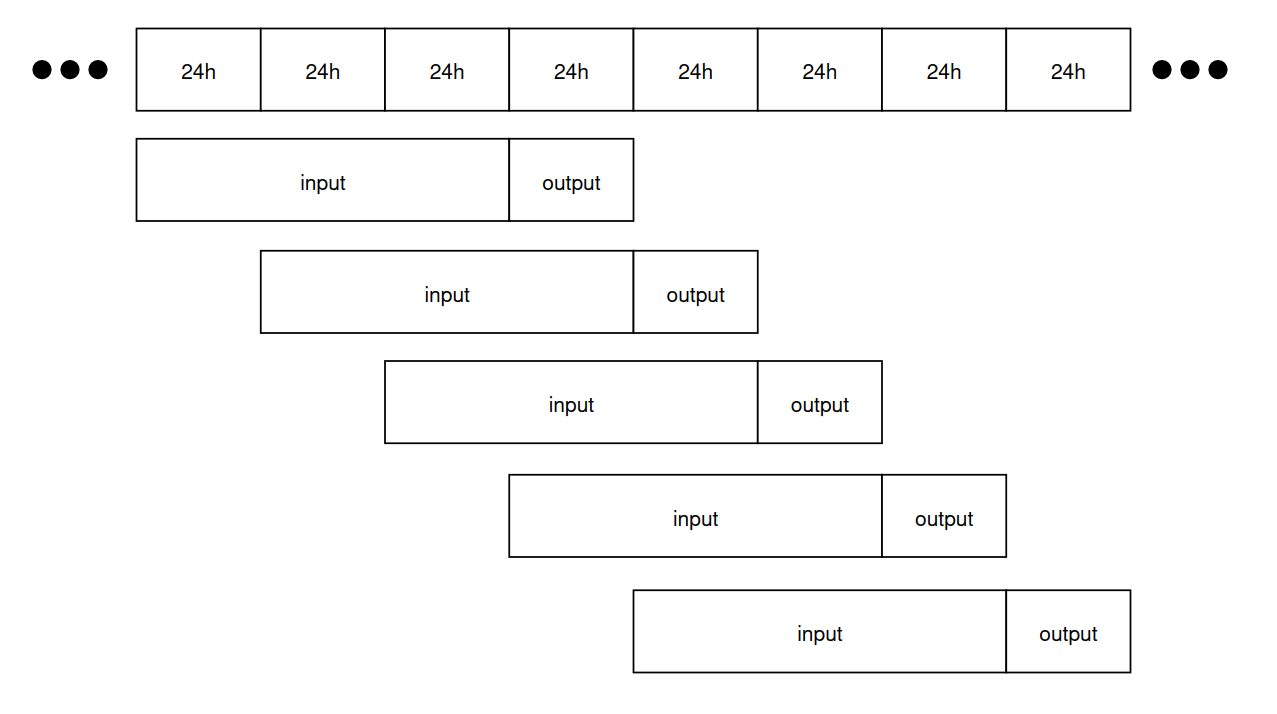
\includegraphics[width=\textwidth]{images/division.png}
    \caption{Sposób podziału zbioru danych na dane wejściowe i~wyjściowe}
    \label{division}
\end{figure}


% Model development: Explain how you developed the models used for your 
% analysis. Discuss the algorithmic choices and parameter settings, 
% as well as any tuning or optimization steps.
\subsection{Zaprojektowanie modelu}

W celu znalezienie hiperparametrów zapewniających najlepszą dokładność modelu,
dwie metody przeszukiwania przestrzeni możliwych wartości zostały zastosowane:

\begin{itemize}
    \item Grid Search — działa poprzez wyczerpujące przeszukiwanie 
    przestrzeni dostępnych parametrów i~wybiera hiperparametry maksymalizujące
    średnią dokładność z~walidacji krzyżowej dokonanej na zbiorze treningowym.
    \item Halving Grid Search — zoptymalizowana czasowo wersja Grid Search
    przydzielająca początkowo ograniczone ilości zasobów (mniejszą ilość
    danych). W~miarę ewaluacji algorytmu iteracyjnie pomniejszany jest zbiór
    rozważanych hiperparametrów, a~najlepszy dobór ewaluowany jest na coraz większym
    zbiorze danych.
\end{itemize}

Niektóre z~wykorzystanych modeli nie są przystosowane do przeprowadzania 
regresji z~wielowymiarowym wyjściem, przez co konieczne jest stworzenie strategii,
w której dla każdy wymiar wyjściowy wymaga stworzenia osobnego modelu. W~tym przypadku
dostrajanie hiperparametrów jest wykonywane osobno dla każdego wymiaru. Wśród
algorytmów, w~których brakuje wsparcia dla wielowymiarowego wyjścia, należą: 
SVR, Regresja logiczna oraz SGD.

Rozważane wartości hiperparametrów zostały zilustrowane w~tabeli \ref{hiperparametry}.

\begin{table}[H]
    \centering
    \caption{Zbiór rozważanych hiperparametrów} \label{hiperparametry}
    \bigskip
    \begin{tabular}{|p{4cm}|p{4cm}|p{4cm}|}
    \hline
    Model & Parametr & Wartości \\
    \hline
    Regresja Logiczna & Solver & svd, cholesky, lsqr, sparse\_cg, sag, saga, lbfgs \\
    \hline
    \multirow{3}{*}{SVR} & kernel & linear, poly, rbf, sigmoid\\
    \cline{2-3}
     & C & 0.1, 1, 10\\
    \cline{2-3}
        & $\epsilon$ & 0.01, 0.1, 1\\
    \hline
    \multirow{3}{*}{SGD} & penalty & l2, l1, elasticnet\\
    \cline{2-3}
     & loss & squared error, huber, epsilon insensitive, squared epsilon insensitive\\
    \hline
\end{tabular}
\end{table}

\begin{table}[H]
    \centering
    \bigskip
    \begin{tabular}{|m{4cm}|m{4cm}|m{4cm}|}
    \hline
    \multirow{3}{*}{KNN} & weights & uniform, distance\\
    \cline{2-3}
     & algorithm & ball tree, kd tree, brute\\
    \cline{2-3}
        & p & 1, 2, 3, 4\\
    \hline
    \multirow{3}{*}{Gaussian} & $\alpha$ & 1e-10, 1e-5, .01, .1 \\
    \cline{2-3}
    & restarts optimizer & 0, 1, 2, 3, 4\\
    \hline
    \multirow{3}{*}{Drzewo decyzyjne} & splitter & best, random \\
    \cline{2-3}
     & min leafs & 1, 2, 3, 4\\
    \cline{2-3}
     & max depth & None, 5, 10, 15, 20\\
    \hline
    \multirow{2}{*}{MLP} & activation & identity, logistic, tanh, relu \\
    \cline{2-3}
     & solver & lbfgs, sgd, adam\\
    \hline
    \multirow{3}{*}{RNN} & recursive layers & [32, 32], [32, 32, 32], [64, 32] \\
    \cline{2-3}
     & fully connected layers & [32, 32], [32, 32, 32], [64, 32]\\
    \cline{2-3}
     & epochs & 10, 15, 20\\
    \hline
    \multirow{5}{*}{CNN} & convolution layers &                                   [32, 32],
    [32, 32, 32],
    [64, 32],
    [64, 64, 64],
    [128, 128, 64] \\
    \cline{2-3}
     & fully connected layers & 
     [32, 32],
     [32, 32, 32],
     [64, 32],
     [64, 64, 64],
     [128, 128, 64]\\
    \cline{2-3}
     & epochs & 10, 15, 20\\
    \hline
    \multirow{2}{*}{NN} & fully connected layers &                                   [32, 32],
    [32, 32, 32],
    [64, 32],
    [64, 64, 64],
    [128, 128, 64],
    [128, 128, 64, 32]\\
    \cline{2-3}
     & epochs & 10, 15, 20 \\
    \hline

    \end{tabular}
\end{table}

Na poniższym rysunku \ref{arch} pokazano uproszczone architektury sieci głębokich.
Podczas procesu przeszukiwania hiperparametrów jednym z~celów optymalizacji 
było znalezienie właściwej liczby i~wielkości warstw konwolucyjnych, rekurencyjnych
i w~pełni połączonych.

\begin{figure}[H]
    \centering
    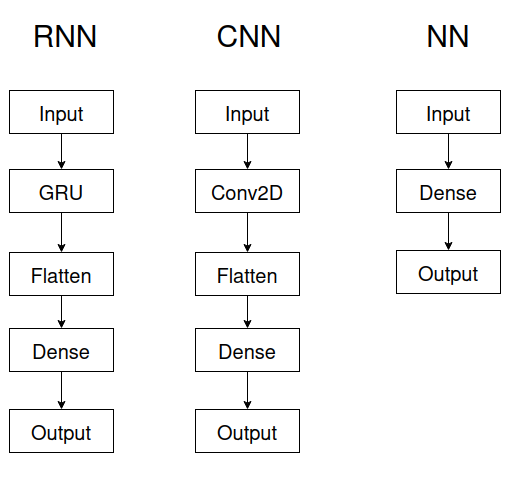
\includegraphics[width=\textwidth]{images/architectures.png}
    \caption[opis dla siatki]{Rysunki poglądowe stworzonych architektur sieci
    głębokich}
    \label{arch}
\end{figure}

% Evaluation metrics: Describe the evaluation metrics you used to 
% measure the performance of your models. Explain why you chose these 
% metrics and how they relate to the research question or problem.
\subsection{Ewaluacja jakości modelu}

Stworzone wytrenowane modele zostały ewaluowane na zbiorze testowym złożonym
z danych meteorologicznych pochodzących ze stycznia z~lat 2020 - 2022.
W celu porównania uzyskanych wyników stworzono zestawienia i~wykresy pokazujące
korelację, błąd średniokwadratowy oraz błąd bezwzględny poszczególnych modeli.

% Code availability: Consider making your code available to others, 
% and provide a~link or repository where readers can access the code 
% you developed. This can facilitate replication of your research and 
% allow others to build upon your work.
\subsection{Dostępność kodu}

Przeprowadzone badania zostały zaimplementowane przy pomocy notatnika Jupyter
\cite{jupyter}, przy pomocy platformy Colab \cite{colab}. Odpowiedni projekt
Jupyter Notebook powinien być dostępny poprzez \url{https://colab.research.google.com/drive/1Fm1UZYe36pVOuCa8jpCKAUoyUJyf3Zmp?usp=sharing}.
% Present the findings of your research. Provide a detailed 
% analysis of the performance of the various algorithms used 
% for weather prediction, including their accuracy, precision, 
% and recall rates.

% The results section of your thesis presents the findings of 
% your study. It should provide a clear and concise summary of 
% the data collected and analyzed, along with any statistical 
% tests or other methods used to analyze the data. Here are some 
% important elements to consider including in your results section:

% Overall, the results section of your thesis should provide a 
% clear and concise summary of your findings, along with any statistical 
% tests or other methods used to analyze the data. It should also provide 
% an interpretation of your findings and relate them back to your research 
% questions or hypotheses.
\section{Wyniki}

% Descriptive statistics: Provide descriptive statistics that 
% summarize the main characteristics of your data, such as means, 
% standard deviations, and frequency distributions.
\subsection{Statystyki}

Jak widać na rysunku \ref{mse}, w przypadku każdego algorytmu nastąpił
spadek dokładności względem danych testowych. W przypadku modelu KNN oraz
regresji gaussowskiej znikomy błąd na danych treningowych wynika z faktu, 
że obydwa modele bazują na uczeniu na przykładach i ich ewaluacja na 
danych treningowych jest niemiarodajna. 

\begin{figure}[H]
    \centering
    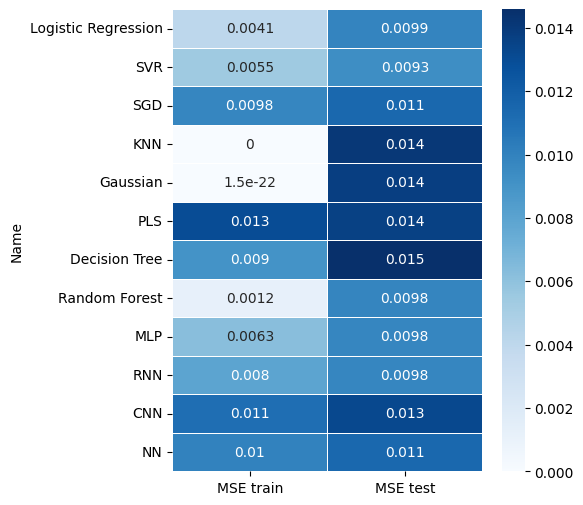
\includegraphics[width=\textwidth]{images/mse.png}
    \caption{Błąd średniokwadratowy dla stworzonych modeli}
    \label{mse}
\end{figure}

Las losowy okazuję się algorytmem, który jest w stanie bardzo dobrze 
dopasować się do danych treningowych razem z zachowaniem ogólności dla 
reszty danych, osiągając dobre wyniki na zbiorze testowym. Z kolei RNN, NN
SVR osiągają zbliżone wartości zarówno dla zbioru treningowego, jak i testowego.

\begin{figure}[H]
    \centering
    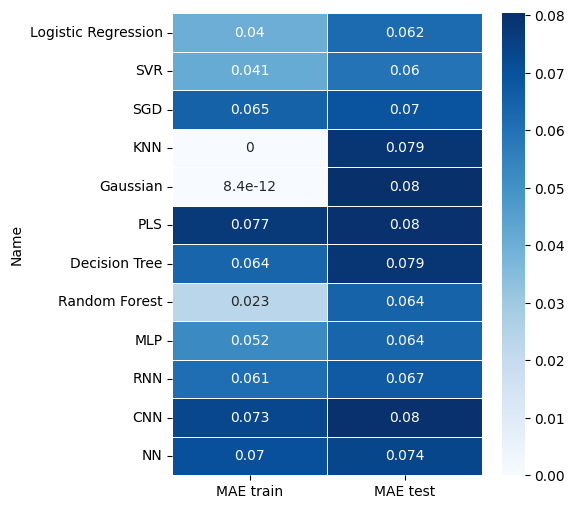
\includegraphics[width=\textwidth]{images/mae.png}
    \caption{Średni błąd absolutny dla stworzonych modeli}
    \label{mae}
\end{figure}

Wartości błędu absolutnego osiągają większe wartości od MSE. Co więcej,
rozbieżność między błędem dla zbioru treningowego i testowego
przy użyciu metryki MAE staje się mniejsza. Ogólna dystrybucja błędu 
względem modeli zdaje się podobna.

\begin{figure}[H]
    \centering
    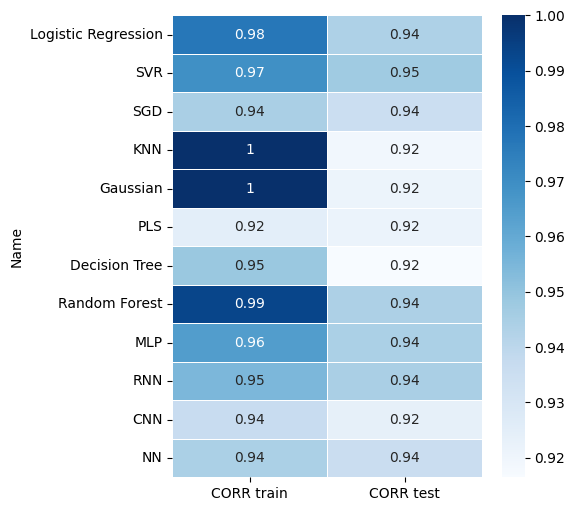
\includegraphics[width=\textwidth]{images/corr.png}
    \caption{Współczynnik korelacji dla stworzonych modeli}
    \label{corr}
\end{figure}

Dla wszystkich modeli współczynnik korelacji pomiędzy wartościami rzeczywistymi 
a przewidzianymi jest na poziomie przekraczającym 0,9. Wskazuje to na dobre dopasowanie
modeli do przewidzianych danych, chociaż warto wskazać, że współczynnik
autokorelacji dla wielu parametrów pozostawał na poziomie powyżej 0,8 dla wartości
opóźnienia przekraczających parę godzin.

\begin{figure}[H]
    \centering
    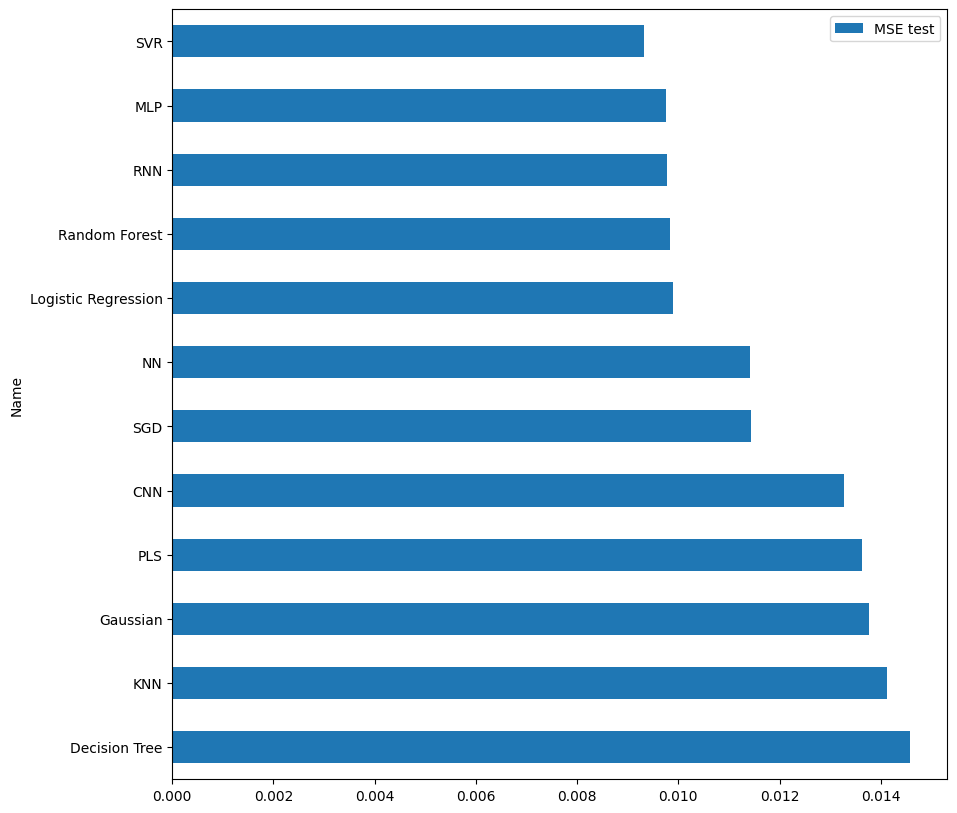
\includegraphics[width=\textwidth]{images/mse_ranking.png}
    \caption{Ranking stworzonych modeli ze względu na błąd średniokwadratowy}
    \label{mse-ranking}
\end{figure}

Na wykresie \ref{mse-ranking} widać stworzony ranking ze względu na wartość MSE.
Najlepszymi algorytmami pod tym względem okazały się SVR, MLP i RNN. Rozbieżność 
pomiędzy najlepszym modelem a najgorszym wynosiła 0,0057. Algorytmami 
osiągającymi najgorsze wyniki był KNN i drzewo decyzyjne.

Można przeprowadzić podobną analizę ze względu na MAE, co zostało pokazane na 
rysunku \ref{mae-ranking}. W tym przypadku o wiele lepsze wyniki 
otrzymała regresja logistyczna i las losowy, które znajdują się wśród najlepiej 
ocenionych algorytmów.

\begin{figure}[H]
    \centering
    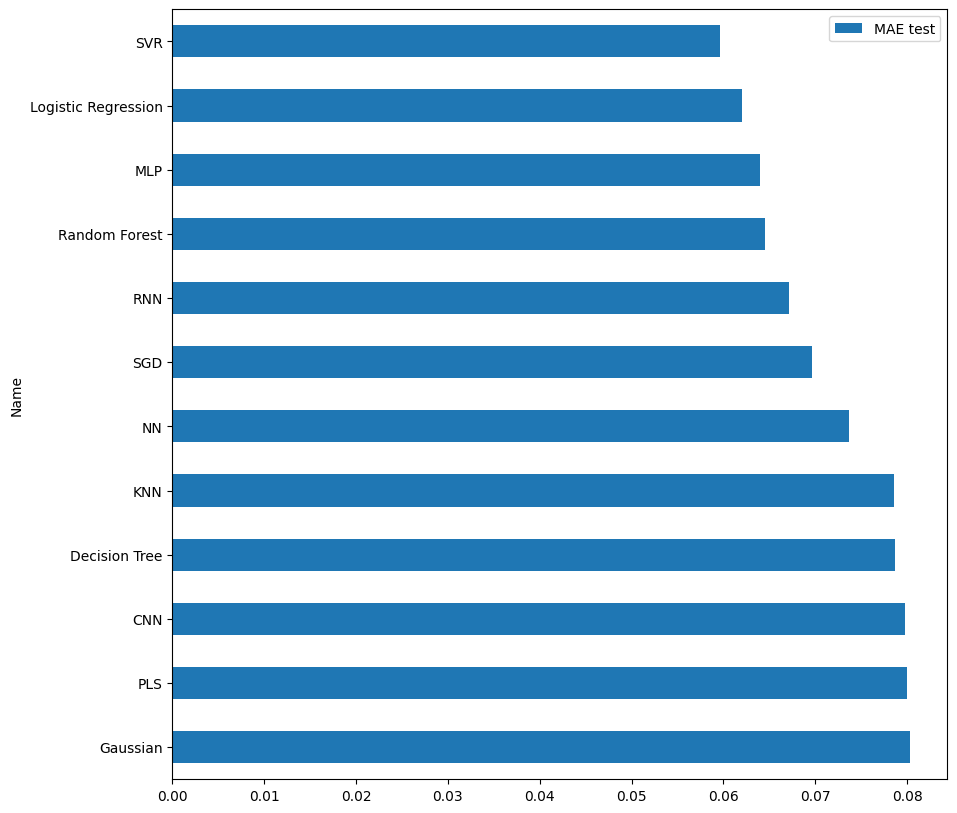
\includegraphics[width=\textwidth]{images/mae_ranking.png}
    \caption{Ranking stworzonych modeli ze względu na średni błąd absolutny}
    \label{mae-ranking}
\end{figure}

Analiza ze względu na korelację pokazuje bardzo zbliżone wartości dla wszystkich 
modeli, a kolejność algorytmów w pokazanym rankingu \ref{corr-ranking} jest 
bardzo podobna do tej ze względu na błąd średniokwadratowy \ref{mse-ranking}.

\begin{figure}[H]
    \centering
    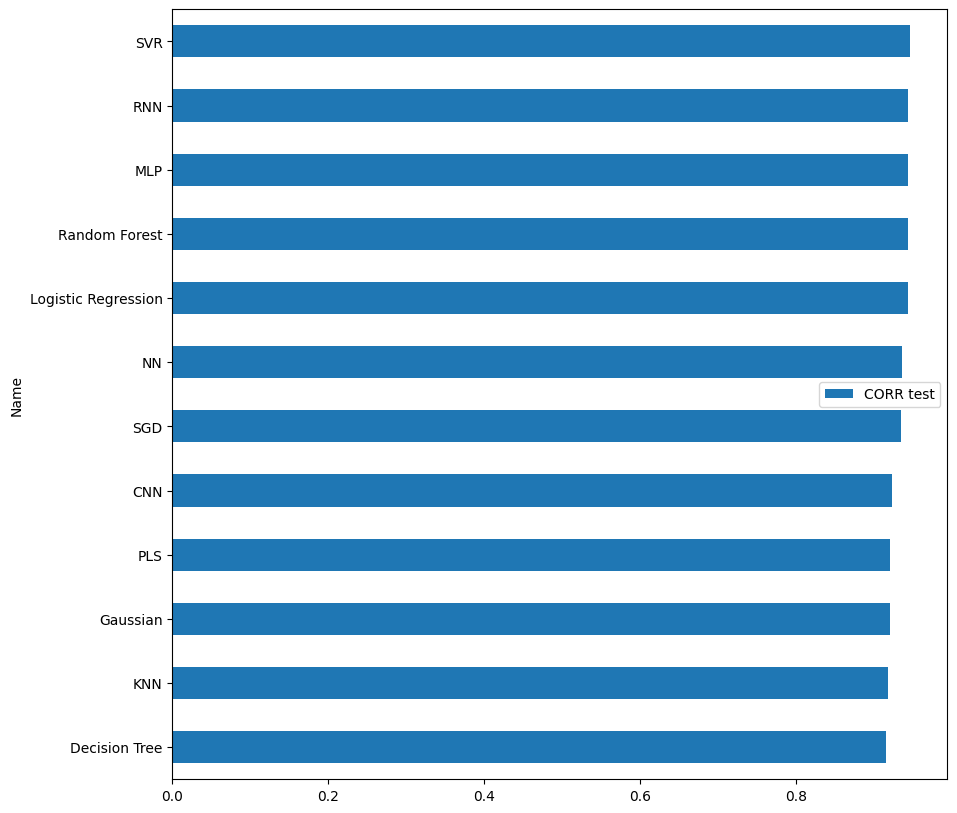
\includegraphics[width=\textwidth]{images/corr_ranking.png}
    \caption{Ranking stworzonych modeli ze względu na wartość korelacji}
    \label{corr-ranking}
\end{figure}

W celu dalszego przybliżenia zachowania poszczególnych modeli, stworzone zostały
zestawienia prawdziwych przebiegów czasowych oraz tych wygenerowanych przez algorytmy
uczenia maszynowego. Chociaż zaprezentowane metryki dają wstępne zrozumienie
stopnia dopasowania modeli oraz ich dokładności, to analiza graficzna jest kluczowa
do zrozumienia, jakie zjawiska są dobrze prognozowane, a jakie stwarzają problemy.
Przedstawione przebiegi prezentują tygodniowe przebiegi złożone z siedmiu 
dwudziestoczterogodzinnych prognoz.

\pagebreak

Jednym z najlepiej ocenianych algorytmów była regresja wektorów wspierających.
W tym przypadku widzimy dobre zachowanie względem przebiegów cyklicznych, takich jak
promieniowanie słoneczne czy odparowanie. Pod względem promieniowania termicznego
widoczne jest dobre odwzorowanie wartości średniej szeregu czasowego, lecz problem
z dopasowaniem do indywidualnych skoków w wartościach.

Nagły skok w wartości opadów został zupełnie pominięty w prognozie i wskazuje 
na problemy z przewidywaniem nagłych zdarzeń o dużej amplitudzie. 

Zarówno wartości prędkości wiatru, jak i temperatury zostały wiernie odwzorowane
przez stworzony model, a na poniższych wykresach widać jak linie prognozowanych wartości
podążają za wartościami przewidywanymi. W przypadku ciśnienia atmosferycznego,
po nagłym spadku model był w stanie dopasować się ponownie do danych pomiarowych
i dalej podążać za utworzonym trendem.

\begin{figure}[H]
    \centering
    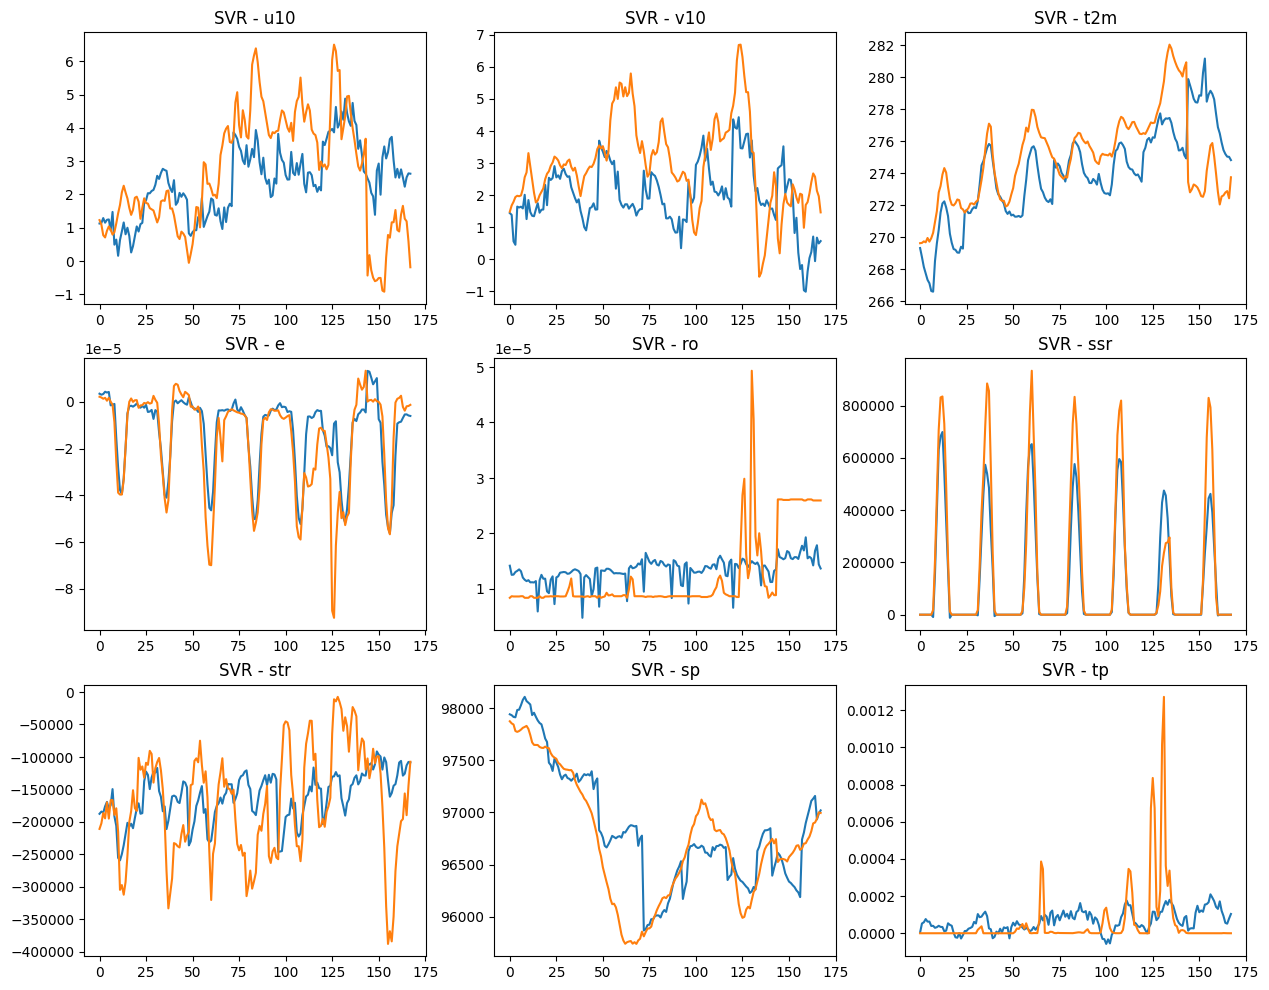
\includegraphics[width=\textwidth]{images/SVR_week.png}
    \caption{Przebiegi czasowe dla algorytmu SVR. Na żółto pokazane zostały dane 
    rzeczywiste, na niebiesko predykcje wygenerowane przez model}
    \label{svr-week}
\end{figure}

\begin{figure}[H]
    \centering
    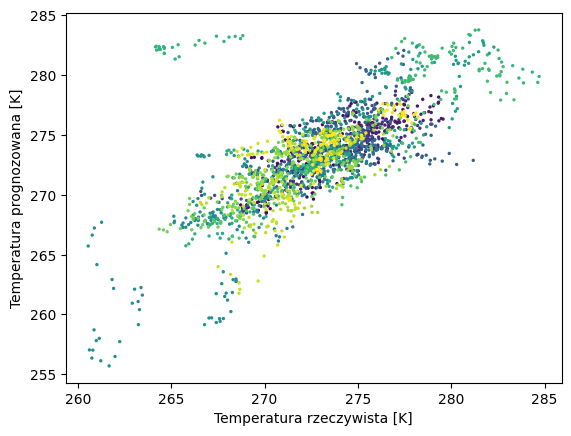
\includegraphics[width=\textwidth]{images/svr_real.png}
    \caption{Scatterplot prezentujący relację pomiędzy prognozowanymi wartościami
    temperatury a wartościami rzeczywistymi dla algorytmu SVR}
    \label{svr-real}
\end{figure}

Na powyższym rysunku \ref{svr-real} pokazano relację pomiędzy rzeczywistymi wartościami
temperatury a wartościami wygenerowanymi przez SVR. Za pomocy gradientu w kolorze wyróżniono postęp
czasowy obserwacji. Widać liniową zależność, zakłócona paroma grupami obserwacji, dla których
odchylenie od wartości rzeczywistych jest największe.

W skrajnym przypadku na powyższym rysunku widać wartości odbiegające o nawet 15 stopni względem
wartości zmierzonych. Warto zanotować także dość dużą wariancję w zbiorze testowym, w którym
temperatura wahała się w zakresie 25 stopni, chociaż wszystkie obserwacje pochodzą ze stycznia.

\pagebreak

Dla perceptronu wielowarstwowego widać dużo większą wariancję w wyjściu modelu 
w zakresie krótkoterminowym. Duże wahania są szczególne widoczne dla wartości odpływów.
Bardzo możliwe, że charakterystyka oscylacyjna danych wejściowych wprowadza znaczną
ilość zakłóceń, a zbyt prosta architektura sieci nie zapewnia możliwości odfiltrowania 
szumów. 

\begin{figure}[H]
    \centering
    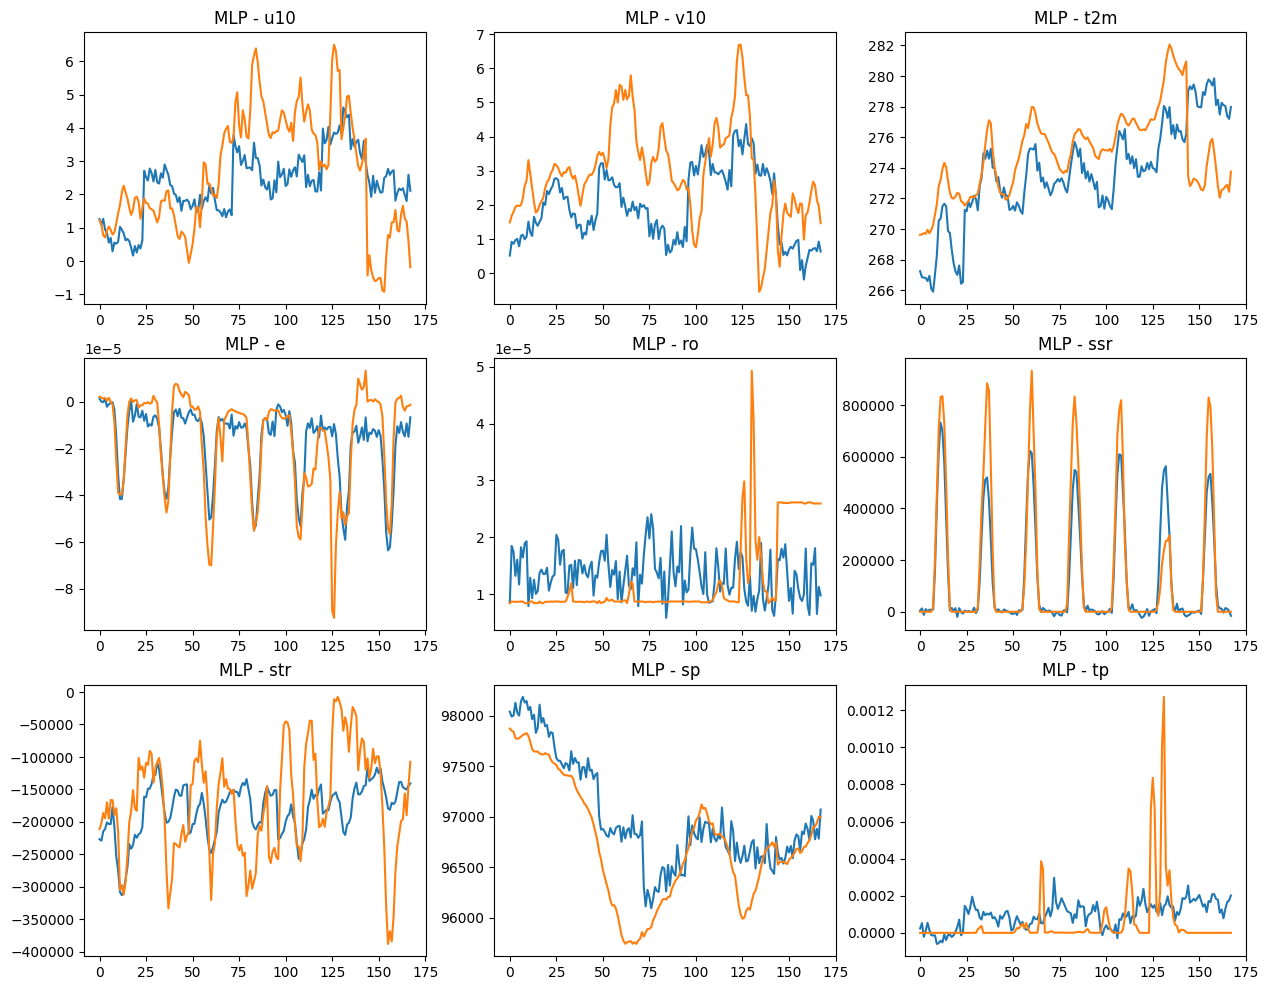
\includegraphics[width=\textwidth]{images/MLP_week.png}
    \caption{Przebiegi czasowe dla algorytmu MLP. Na żółto pokazane zostały dane 
    rzeczywiste, na niebiesko predykcje wygenerowane przez model}
    \label{mlp-week}
\end{figure}

Rekurencyjna architektura sieci neuronowych RNN prezentuje podobne zachowanie, 
generując dane wyjściowe z dużymi wahaniami. Wyniki dla tego modelu zostały zaprezentowane na rysunku \ref{rnn-week}

\begin{figure}[H]
    \centering
    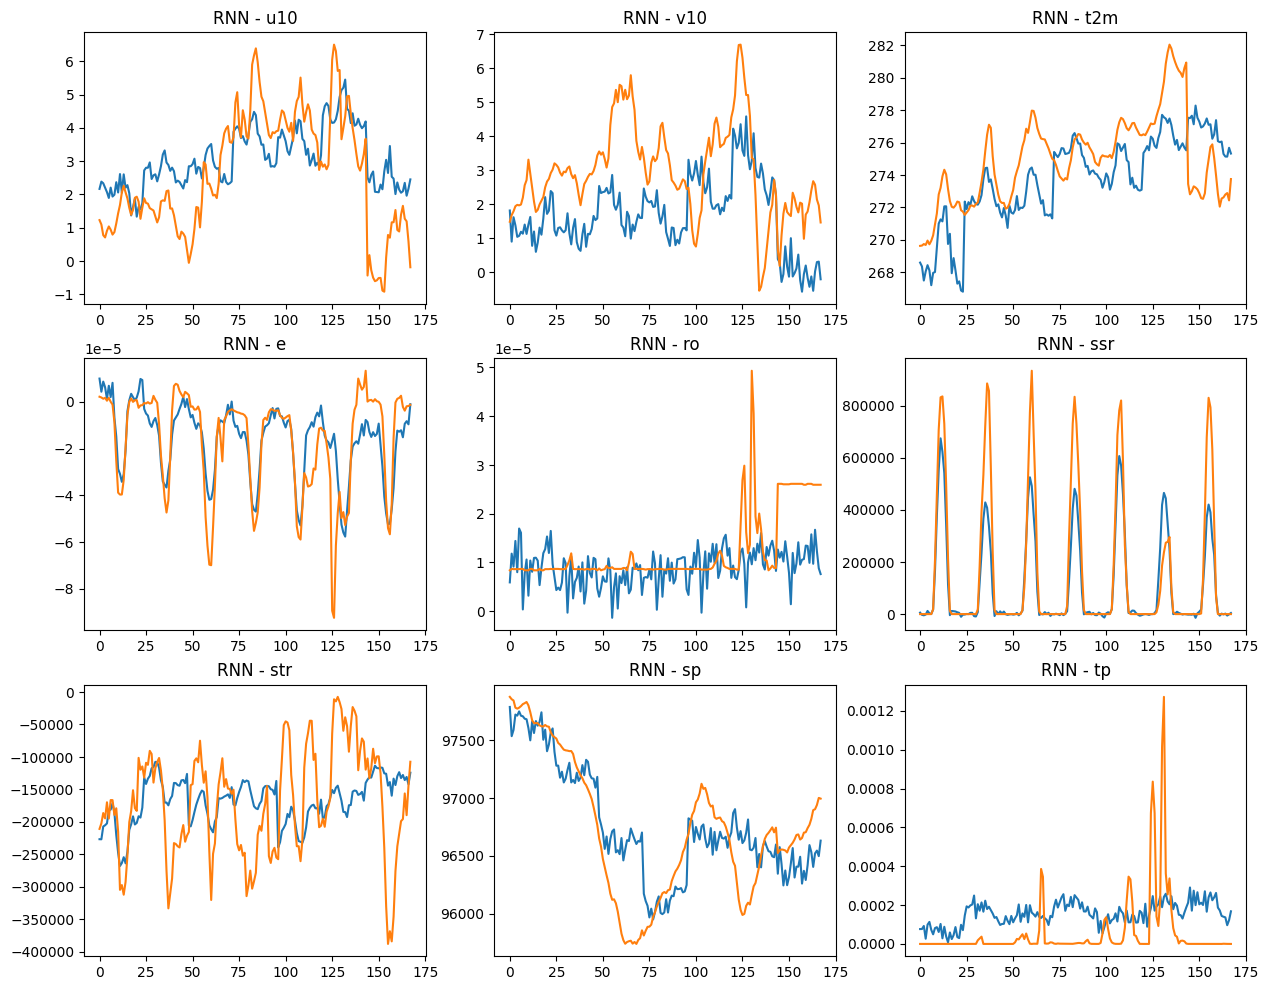
\includegraphics[width=\textwidth]{images/rnn_week.png}
    \caption{Przebiegi czasowe dla algorytmu RNN. Na żółto pokazane zostały dane 
    rzeczywiste, na niebiesko predykcje wygenerowane przez model}
    \label{rnn-week}
\end{figure}

W przypadku lasu losowego widać duże przesunięcie dla linii odpływów wody. Stworzone prognozy zdecydowanie
przeceniają wartości rzeczywiste, co może być spowodowane pojedynczymi zdarzeniami w zbiorze treningowym o
dużej amplitudzie, które mogły zaburzyć proces uczenia modelu.

Można też zauważyć widoczne wahania o charakterze dwudziestoczterogodzinnym w wartościach 
prędkości wiatru i temperatury, które niekoniecznie odnajdują odzwierciedlenie w danych rzeczywistych.

\begin{figure}[H]
    \centering
    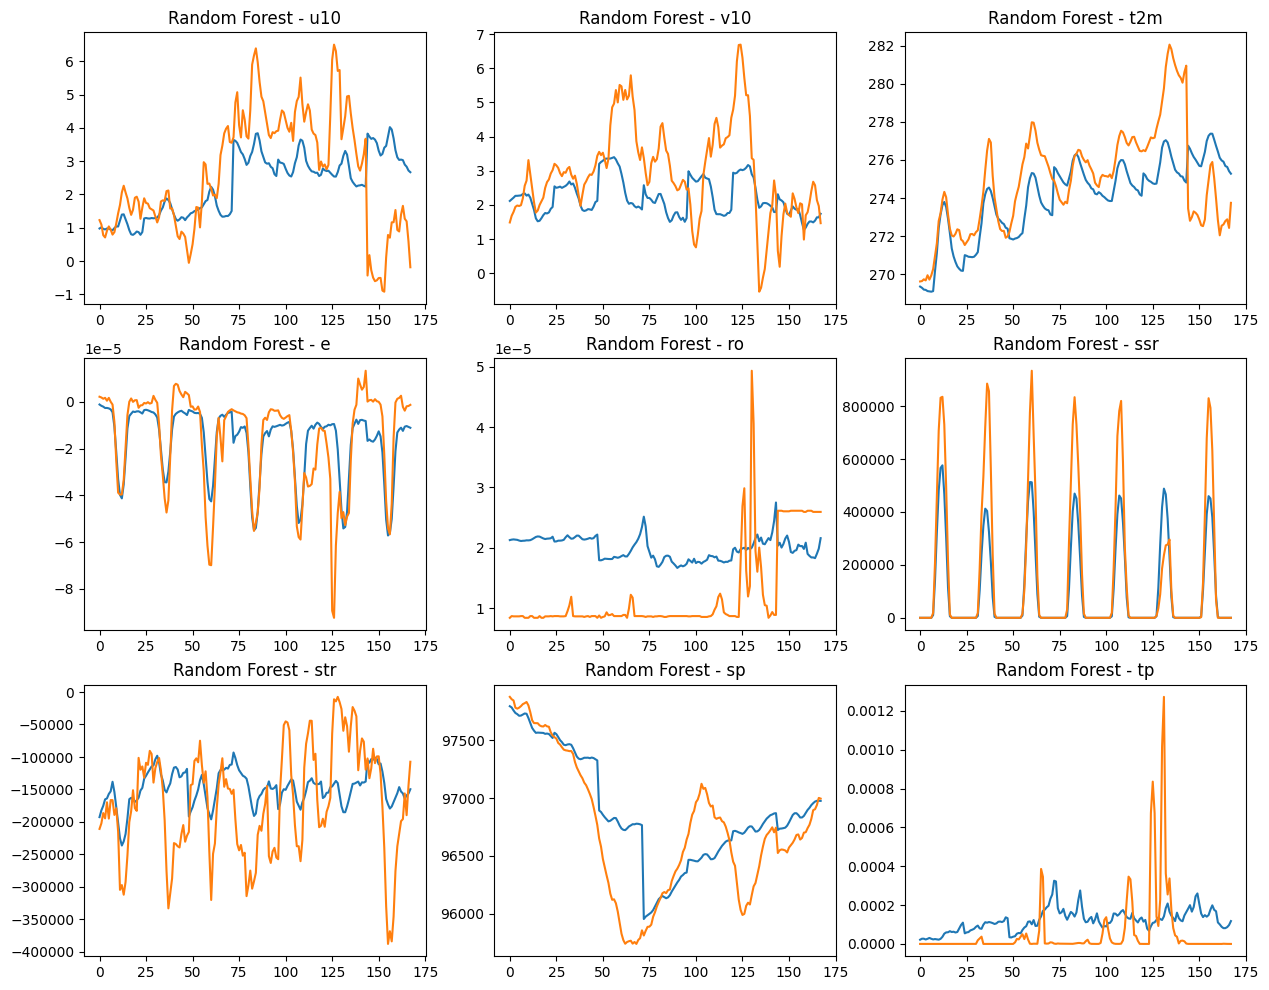
\includegraphics[width=\textwidth]{images/random_forest_week.png}
    \caption{Przebiegi czasowe dla algorytmu lasu losowego. Na żółto pokazane zostały dane 
    rzeczywiste, na niebiesko predykcje wygenerowane przez model}
    \label{forest-week}
\end{figure}

Kolejnym rozważanym modelem jest regresja logistyczna, która wydaje się, najlepiej odzwierciedliła 
zachowania przebiegu temperatury, odparowania i promieniowania słonecznego. Większe wartości 
błędu dla tego modelu mogą być spowodowane gorszym dopasowaniem względem pozostałych parametrów, dla których
często prognozowane są nieprawidłowe wahania od rzeczywistego trendu.

\begin{figure}[H]
    \centering
    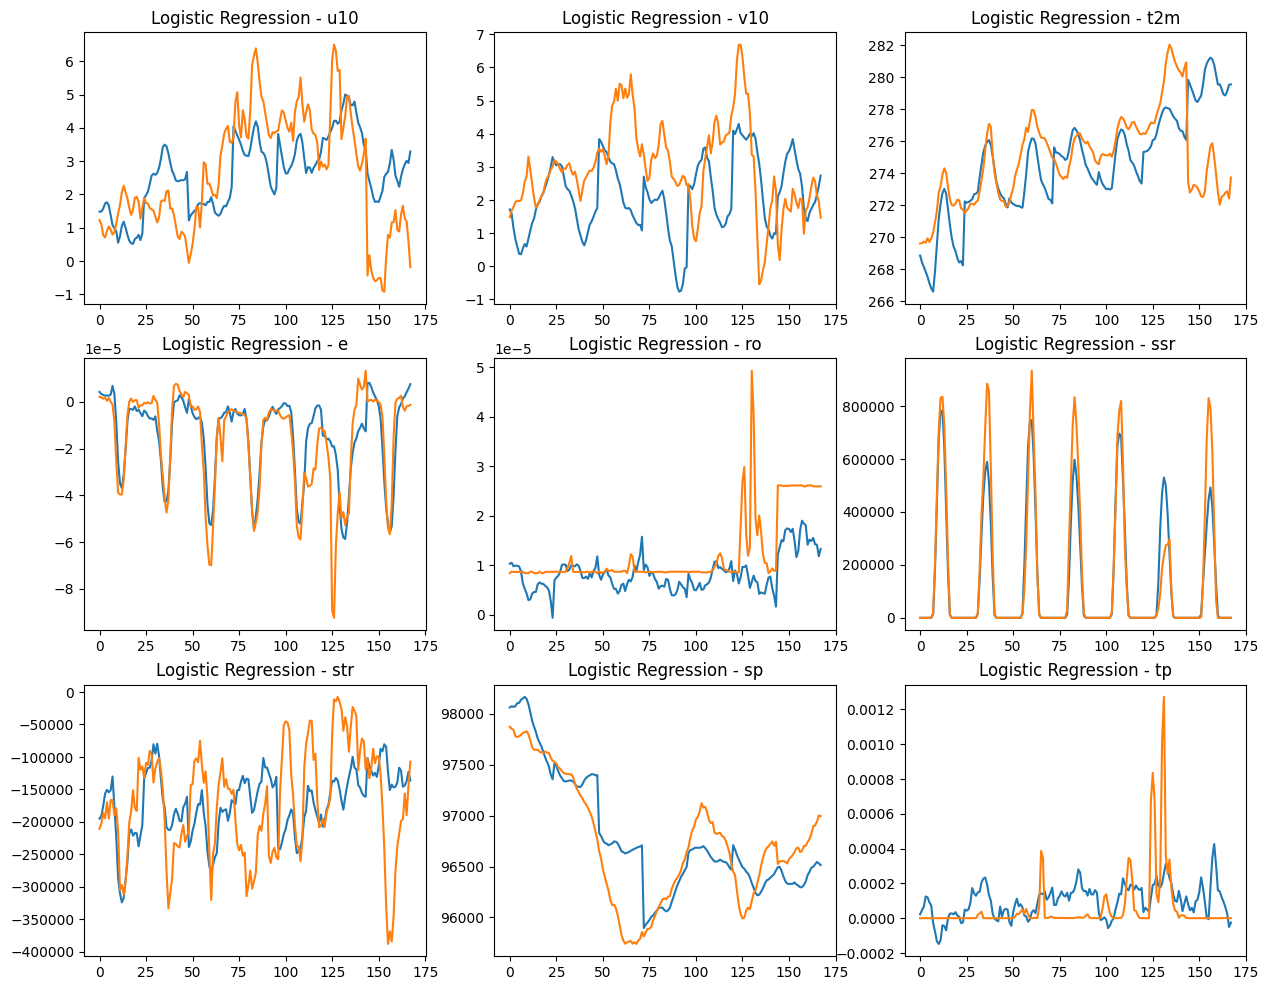
\includegraphics[width=\textwidth]{images/regression_week.png}
    \caption{Przebiegi czasowe dla algorytmu regresji logistycznej. Na żółto pokazane zostały dane 
    rzeczywiste, na niebiesko predykcje wygenerowane przez model}
    \label{regression-week}
\end{figure}

\begin{figure}[H]
    \centering
    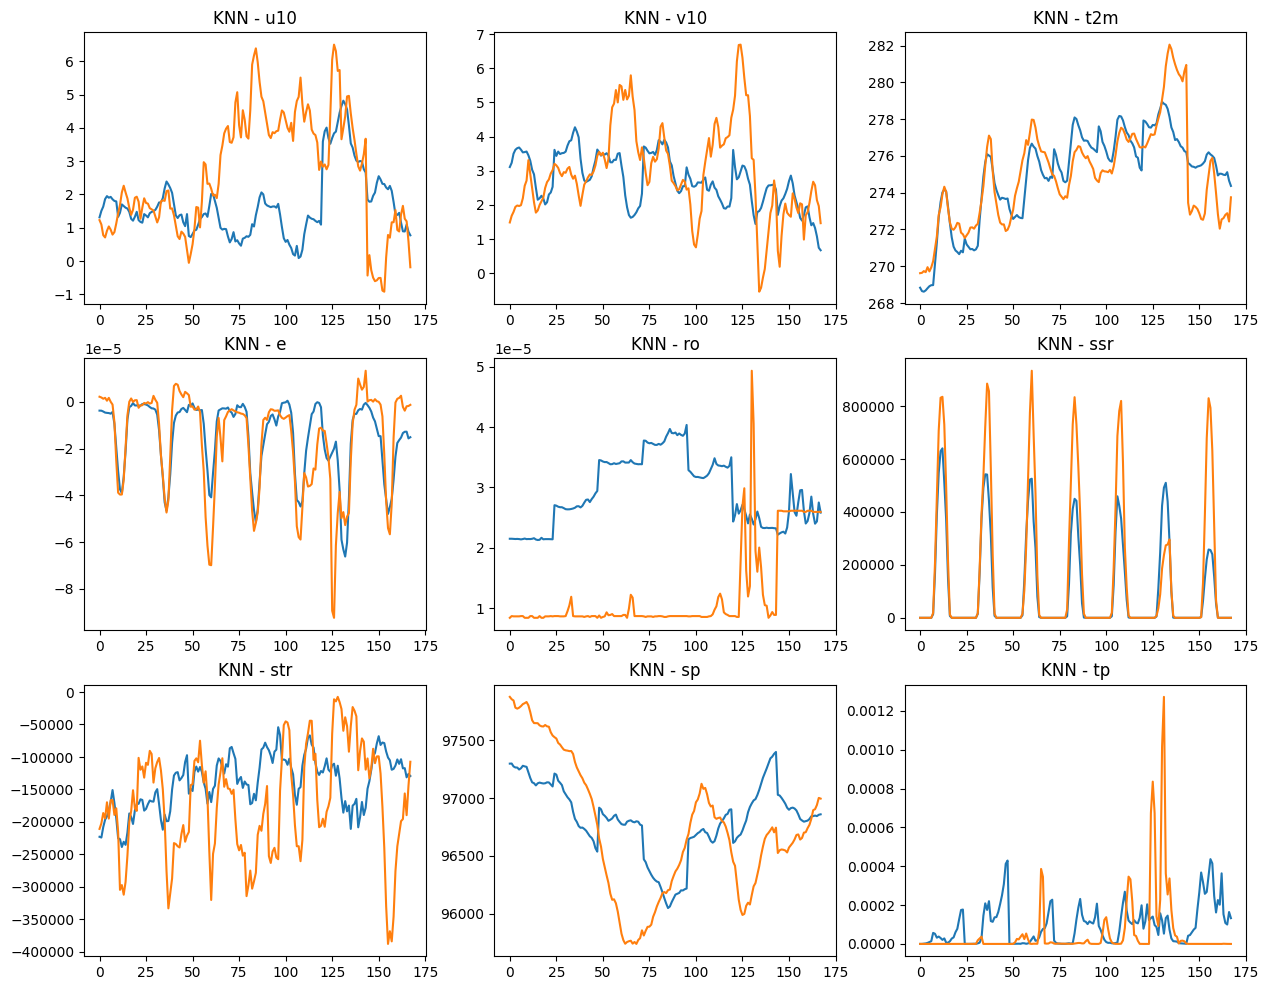
\includegraphics[width=\textwidth]{images/knn_week.png}
    \caption{Przebiegi czasowe dla algorytmu KNN. Na żółto pokazane zostały dane 
    rzeczywiste, na niebiesko predykcje wygenerowane przez model}
    \label{knn-week}
\end{figure}

Algorytm K najbliższych sąsiadów ma wyraźne trudności w rozpoznawaniu danych wejściowych różniących się od 
danych zawartych w zbiorze treningowym. Wyraźne odchylenia widoczne są przede wszystkim w przebiegach  
symbolizujących odpływ i ciśnienie atmosferyczne. Co więcej, bardzo dużo opadów zostało fałszywie
zasygnalizowane. Model KNN okazuje się niestosowny do problemu prognozowania pogody ze względu
na brak generalizacji nabytej wiedzy i dostosowania do nowych danych.

\pagebreak

Można także przeanalizować zdolność poszczególnych modeli do regresji względem poszczególnych atrybutów.
Tak na przykład na rysunku \ref{svr-mse-bar} pokazany został błąd średniokwadratowy dla modelu SVR, który był
jednym z modeli o najlepszych wynikach. Z przedstawionego wykresu wynika, że największy błąd jest generowany
przez prognozowanie promieniowania termicznego. Problemy w regresji względem tego atrybutu mogą być  
spowodowane między innymi jego wysoką wariancją i zależnością od procesów fizycznych nieujętych w zbiorze 
danych.

\begin{figure}[H]
    \centering
    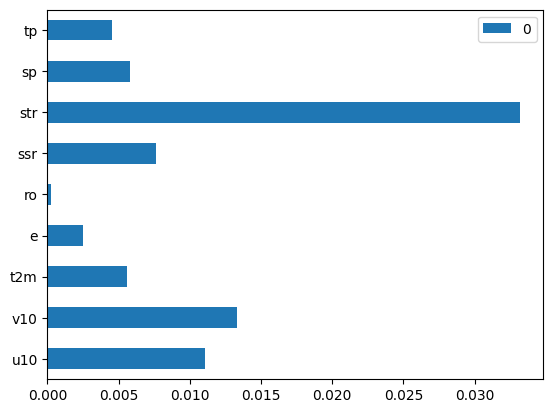
\includegraphics[width=\textwidth]{images/svr_mse_bar.png}
    \caption{Wartości błędu średniokwadratowego dla modelu SVR ze względu na poszczególne atrybuty danych.}
    \label{svr-mse-bar}
\end{figure}

Charakterystyka względem średniego błędu absolutnego wskazuje na te same wnioski. Najcięższymi parametrami
do przewidzenia były wartości promieniowania słonecznego oraz prędkości wiatru. Jednak nie wszystkie
parametry są jednakowo ujęte poprzez zastosowanie tej metryki. Stosując MAE widać, że błędy 
uwzględnione w prognozowaniu promieniowania słonecznego są mniejsze niż te wywołane przez ciśnienie
atmosferyczne oraz ilość opadów. Jest to przykład tego, jak używanie różnych metryk może prowadzić do 
odmiennych wniosków i być przyczyną odmiennej interpretacji.

\begin{figure}[H]
    \centering
    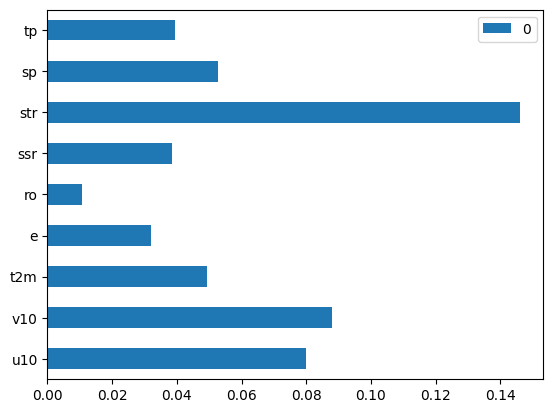
\includegraphics[width=\textwidth]{images/svr_mae_bar.png}
    \caption{Wartości średniego błędu absolutnego dla modelu SVR ze względu na poszczególne atrybuty danych.}
    \label{svr-mae-bar}
\end{figure}

Ponieważ MSE jest bardziej krytyczną metryką względem krótkotrwałych odchyleń o dużej różnicy względem
danych rzeczywistych, możemy wnosić, że różnice w danych generowanych dla wartości promieniowania słonecznego
mają charakter chwilowy, a po porównaniu wykresów szeregów czasowych widać, że największym problem okazuje
się prognozowanie wartości maksymalnej dla poszczególnych dni.

\pagebreak

% Inferential statistics: Report the results of any inferential 
% statistical analyses that you conducted to test your research 
% hypotheses, such as t-tests, ANOVA, regression analysis, or 
% other statistical tests. Be sure to include the statistical 
% significance of the results and the effect sizes.
\subsection{Analiza dystrybucji i korelacji}

W celach dalszej eksploracji otrzymanych wyników przeprowadzone zostało porównanie dystrybucji 
rzeczywistych parametrów atmosferycznych z predykcjami wygenerowanymi przez rozpatrywane algorytmy.
Na poniższym rysunku \ref{real-hist} zostały ponownie przedstawione histogramy dla oryginalnych danych pomiarowych.

\begin{figure}[H]
    \centering
    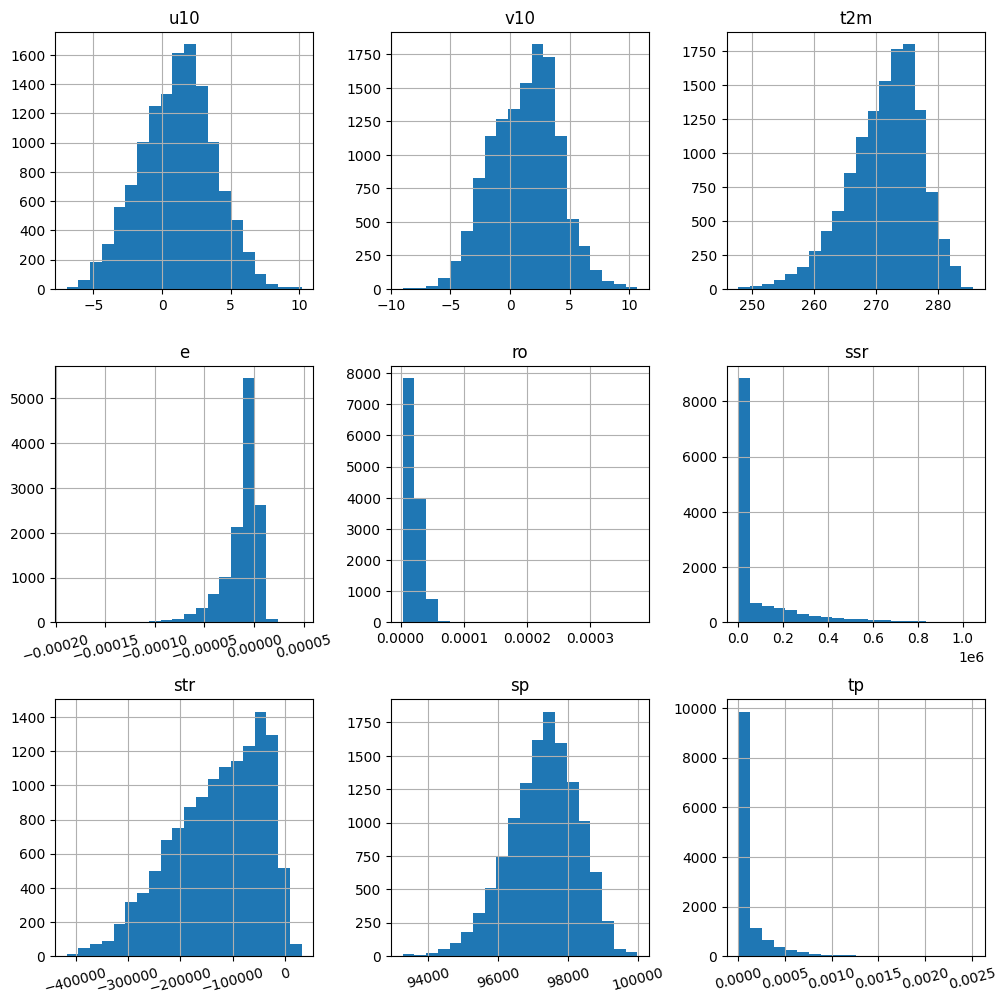
\includegraphics[width=\textwidth]{images/hist.png}
    \caption{Histogramy prezentujące dystrybucję danych rzeczywistych}
    \label{real-hist}
\end{figure}

Widzimy regularność w przedstawionych danych i choć nie wszystkie atrybuty podążają za dystrybucją normalną 
oraz występuje skośność w danych, to istnieje jednoznaczny model tworzący istniejące dane.

Nawet inspekcja najlepiej działającego algorytmu, którym jest SVR, pokazuje wady w utworzonych 
prognozach. Nieregularność dystrybucji danych szczególnie widoczna dla odpływów wody oraz
ciśnienia atmosferycznego ujawniają syntetyczne pochodzenie wygenerowanych predykcji. 
Co więcej, odparowanie, promieniowanie termiczne oraz ilość odpadów odbiegają od oryginalnego kształtu
dystrybucji danych.

\begin{figure}[H]
    \centering
    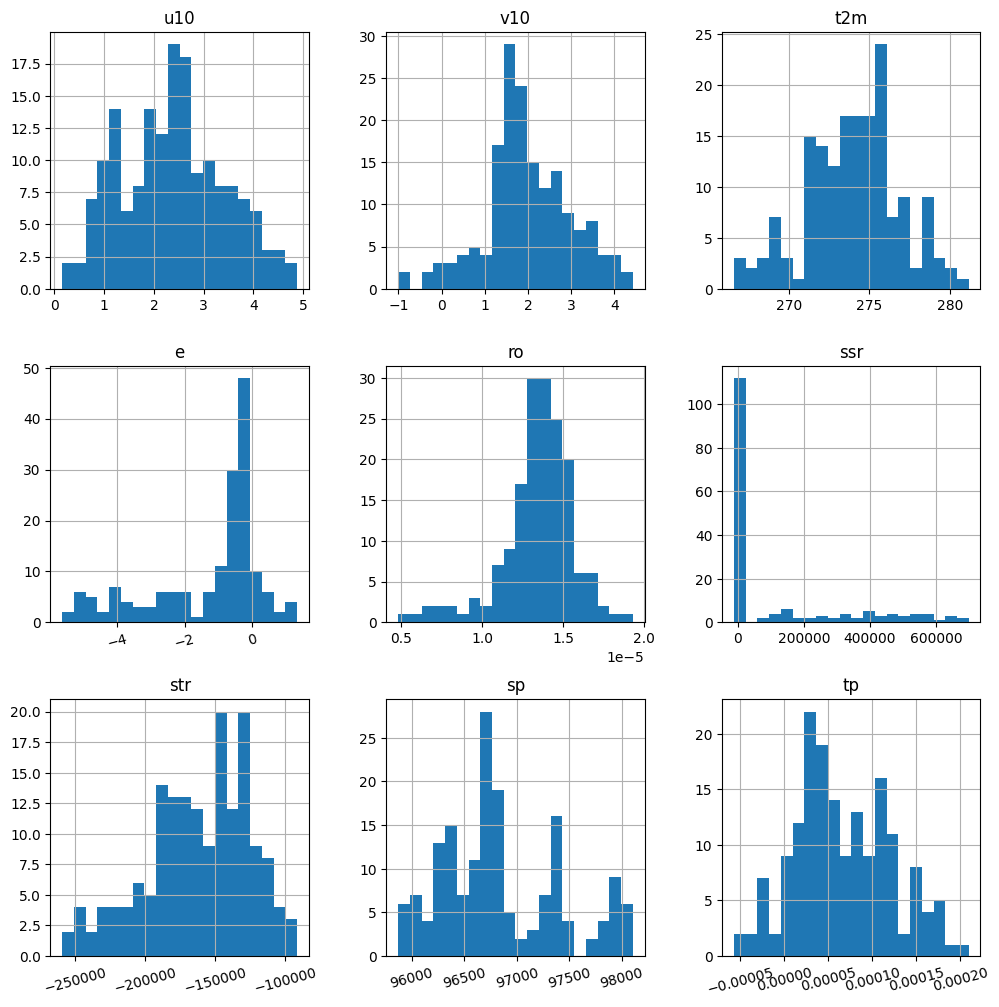
\includegraphics[width=\textwidth]{images/svr_hist.png}
    \caption{Histogramy prezentujące dystrybucję predykcji wygenerowanych przez algorytm SVR.}
    \label{svr-hist}
\end{figure}

\begin{figure}[H]
    \centering
    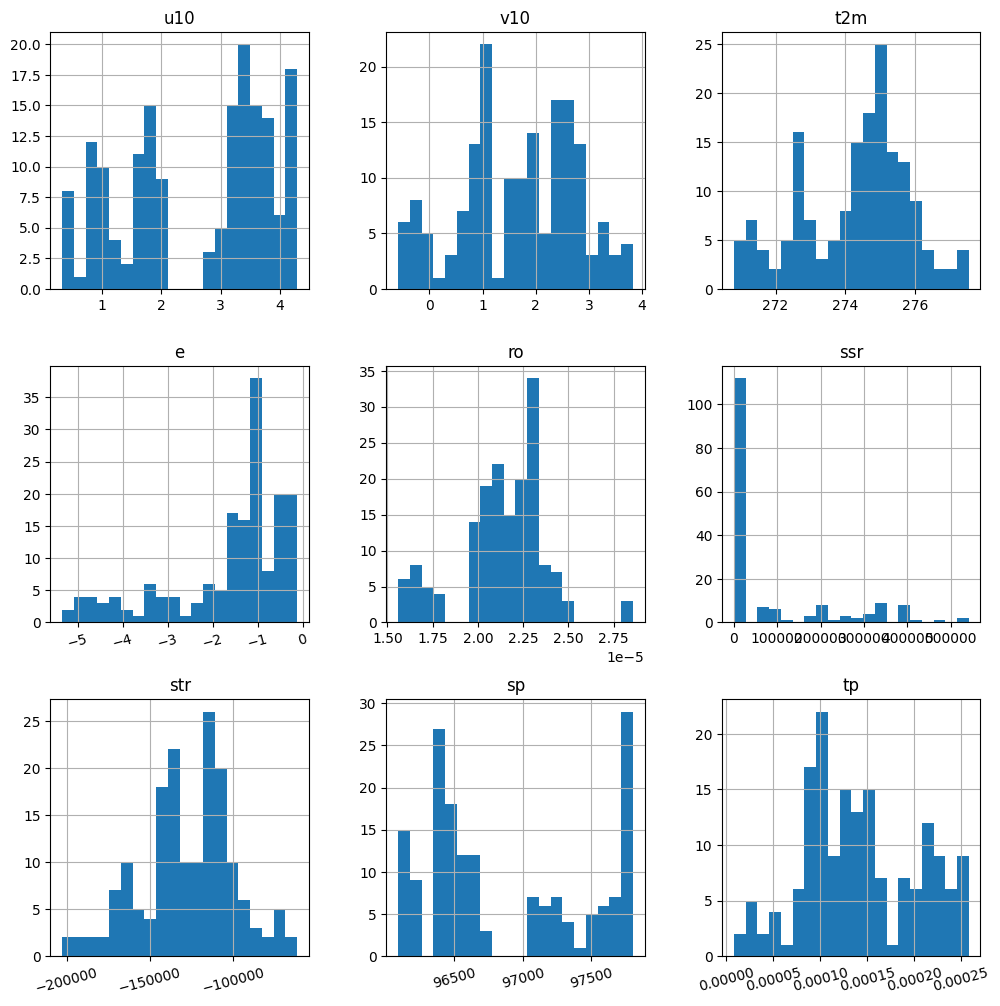
\includegraphics[width=\textwidth]{images/dt_hist.png}
    \caption{Histogramy prezentujące dystrybucję predykcji wygenerowanych przez algorytm drzewo decyzyjne.}
    \label{dt-hist}
\end{figure}

Na rysunku \ref{dt-hist} pokazane zostały analogiczne dystrybucje dla drzewa decyzyjnego. Luki w 
pewnych zakresach danych oraz brak ciągłości w dystrybucji ujawnia złe modelowanie zjawisk atmosferycznych,
poprzez nieprawidłowe odwzorowanie danych rzeczywistych. 

\begin{figure}[H]
    \centering
    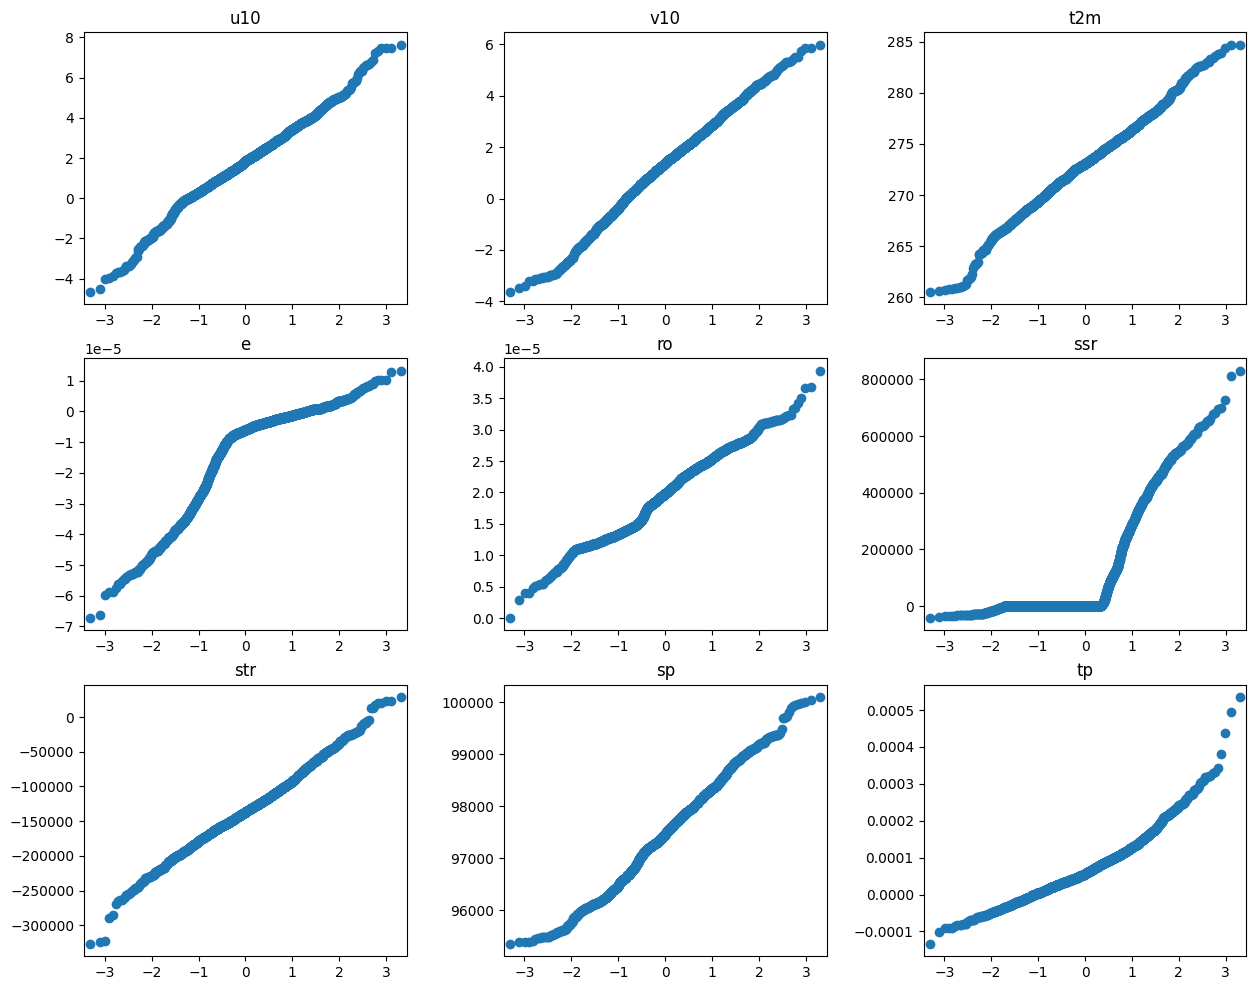
\includegraphics[width=\textwidth]{images/svr_qq.png}
    \caption{Wykresy QQ stworzone dla modelu SVR}
    \label{svr-qq}
\end{figure}

Aby przeprowadzić dalszą analizę, stworzone zostały wykresy QQ pokazane na rysunku \ref{svr-qq} oraz \ref{dt-qq}.
W przypadku algorytmu SVR większość danych podąża za dystrybucją normalną, nawet w przypadkach,
gdy dla danych rzeczywistych nie było to prawdą. Wyjątkiem od tego są odparowanie oraz promieniowanie 
termiczne, które odbiegają od ogólnego trendu i zdają się sumą dwóch dystrybucji normalnych.

Analogiczny wykres dla drzewa decyzyjnego pokazuje chaotyczność w wytworzonych danych, jeszcze raz 
udowadniając niestosowność zastosowanego algorytmu. Poprzez użycie drzewa decyzyjnego reprodukcja
rzeczywistych parametrów jest niemożliwa, a utworzone prognozy pogodowe odbiegają od oczekiwanych wartości.

\begin{figure}[H]
    \centering
    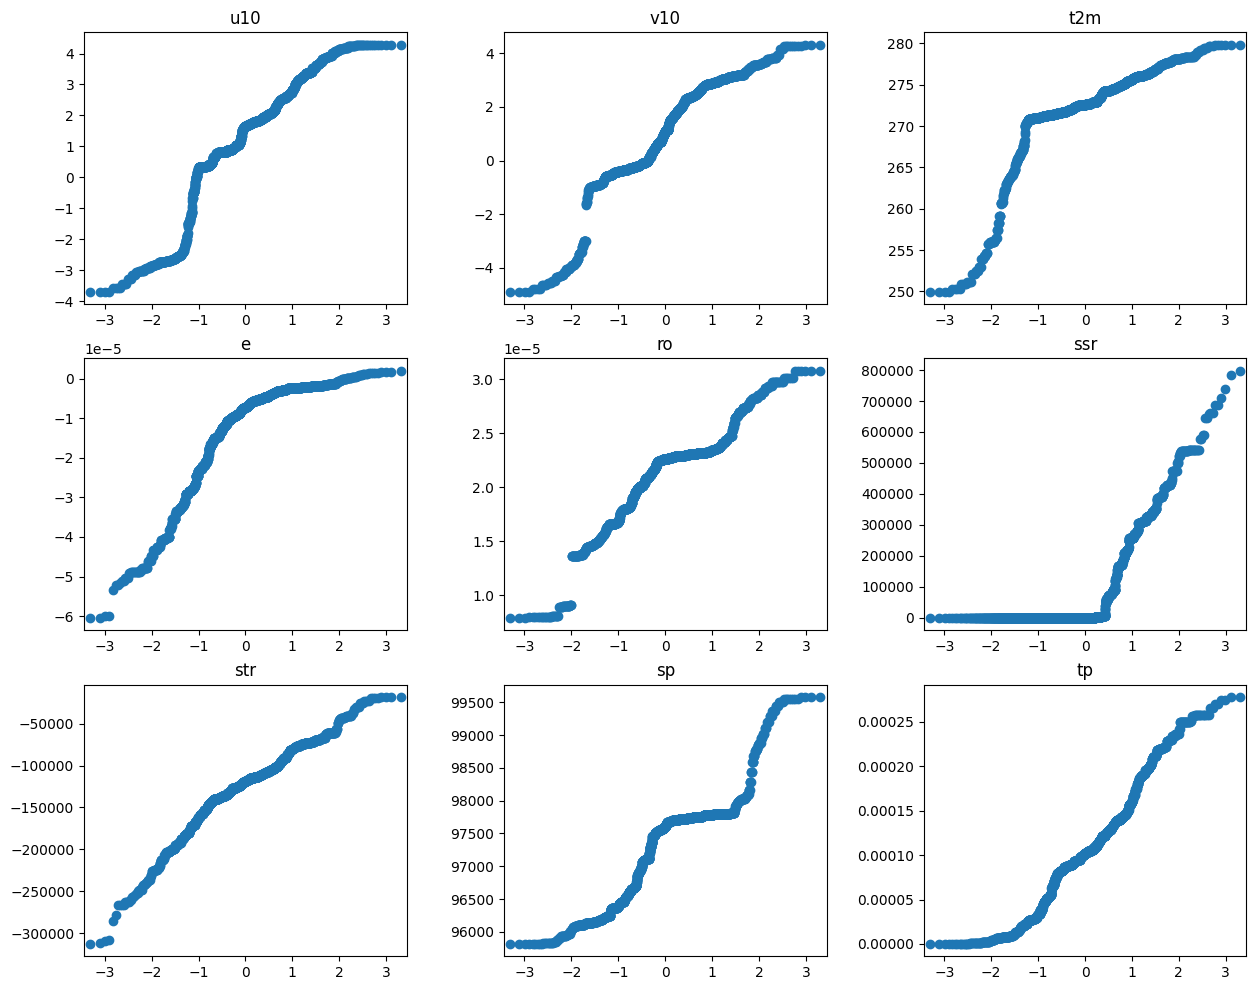
\includegraphics[width=\textwidth]{images/dt_qq.png}
    \caption{Wykresy QQ stworzone dla modelu drzewa decyzyjnego}
    \label{dt-qq}
\end{figure}

Kolejnym pokazanym rysunkiem są wykresy pudełkowe dla algorytmu SVR pokazane na zdjęciu \ref{svr-box}. 
Widzimy na nich o wiele mniejszą ilość
danych odstających w stosunku do tych samych wykresów wygenerowanych dla danych rzeczywistych. Co więcej,
większość parametrów zdaje się posiadać symetryczny rozkład, co nie było prawdą dla modelowanych danych.

\begin{figure}[H]
    \centering
    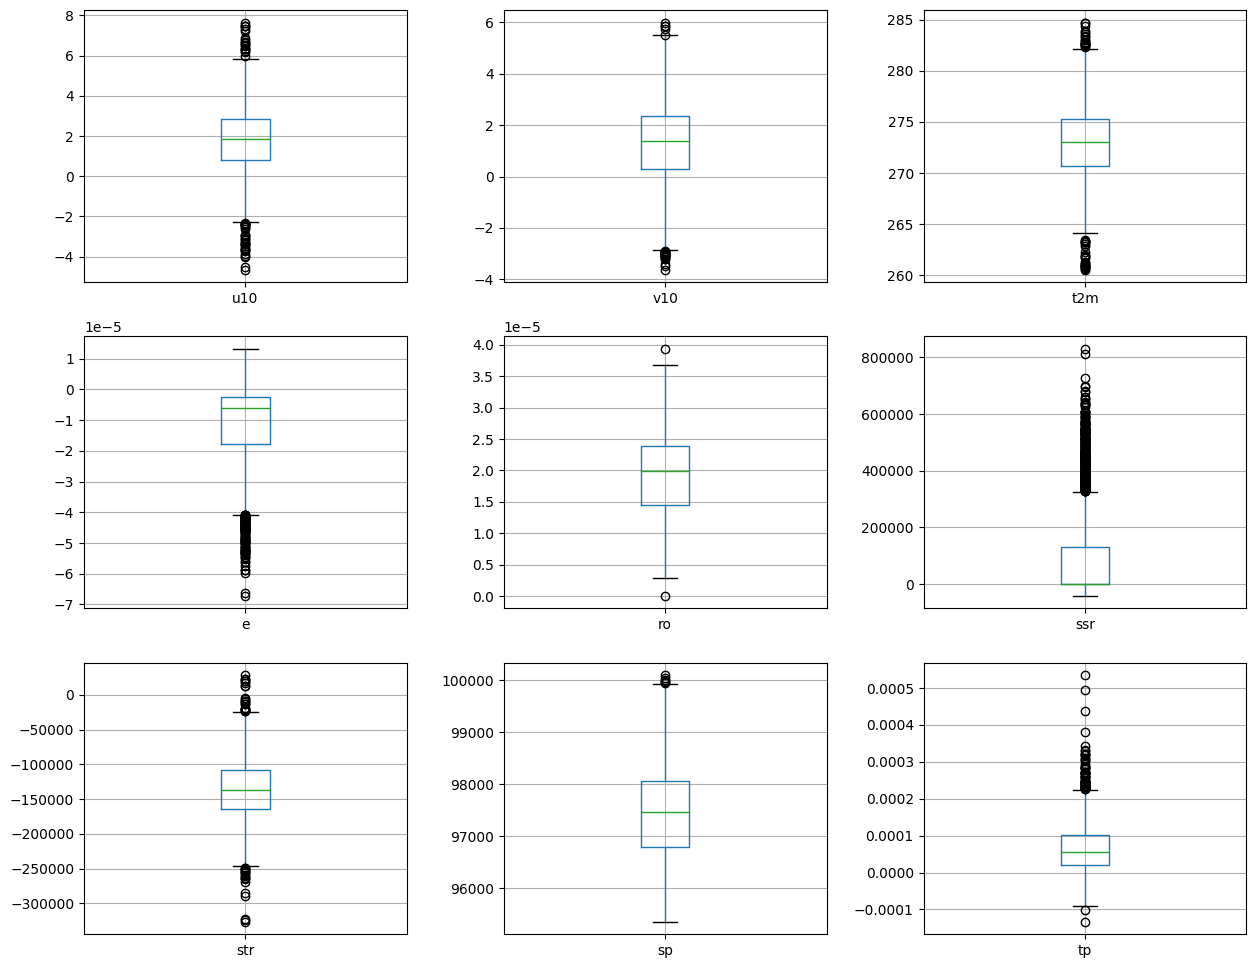
\includegraphics[width=.8\textwidth]{images/svr_box.png}
    \caption{Wykresy pudełkowe dla modelu SVR}
    \label{svr-box}
\end{figure}

\begin{figure}[H]
    \centering
    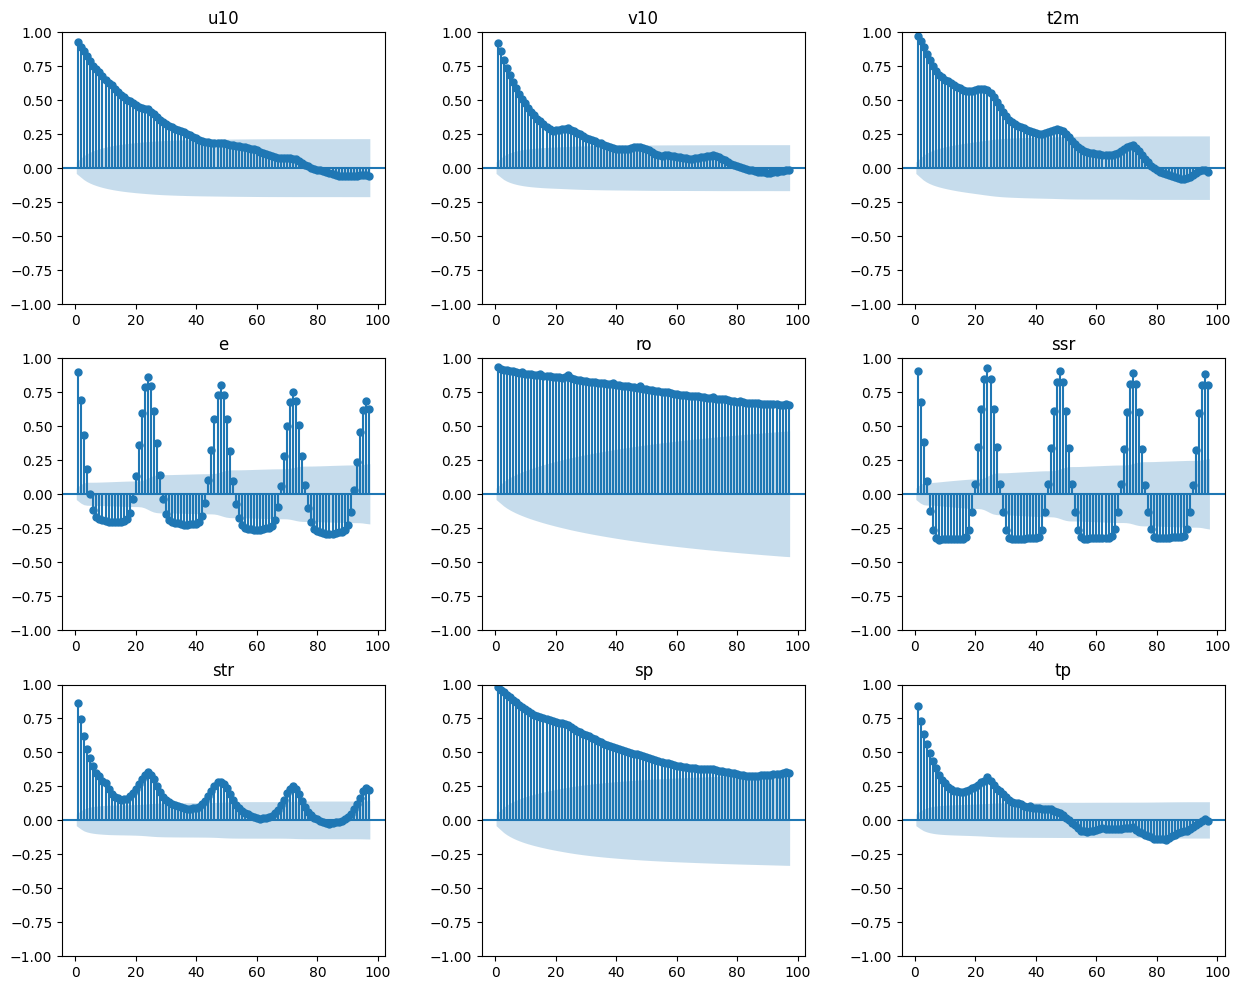
\includegraphics[width=.8\textwidth]{images/svr_autocorr.png}
    \caption{Współczynnik autokorelacji dla SVR dla wartości przesunięcia w zakresie czterech dni}
    \label{svr-autocorr}
\end{figure}

Obserwując wykresy autokorelacji, możemy także zaobserwować zależności, które nie występowały pierwotnie w 
zbiorze danych. Pierwotnie szeregi czasowe dla prędkości wiatru nie ujawniały natury cyklicznej, jednak 
na wykresie \ref{svr-autocorr} widać periodyczne skoki w wartości autokorelacji następujące co jeden dzień.
Ten sam wniosek może zostać wyciągnięty względem ilości opadów, które dla analizowanego zbioru danych 
ujawniały jednostajnie spadającą autokorelację, a w tym przypadku widzimy nieregularny przebieg z okresowymi
skokami. Mimo to wartości dla reszty atrybutów są bardzo bliskie względem symulowanych danych.

\begin{figure}[H]
    \centering
    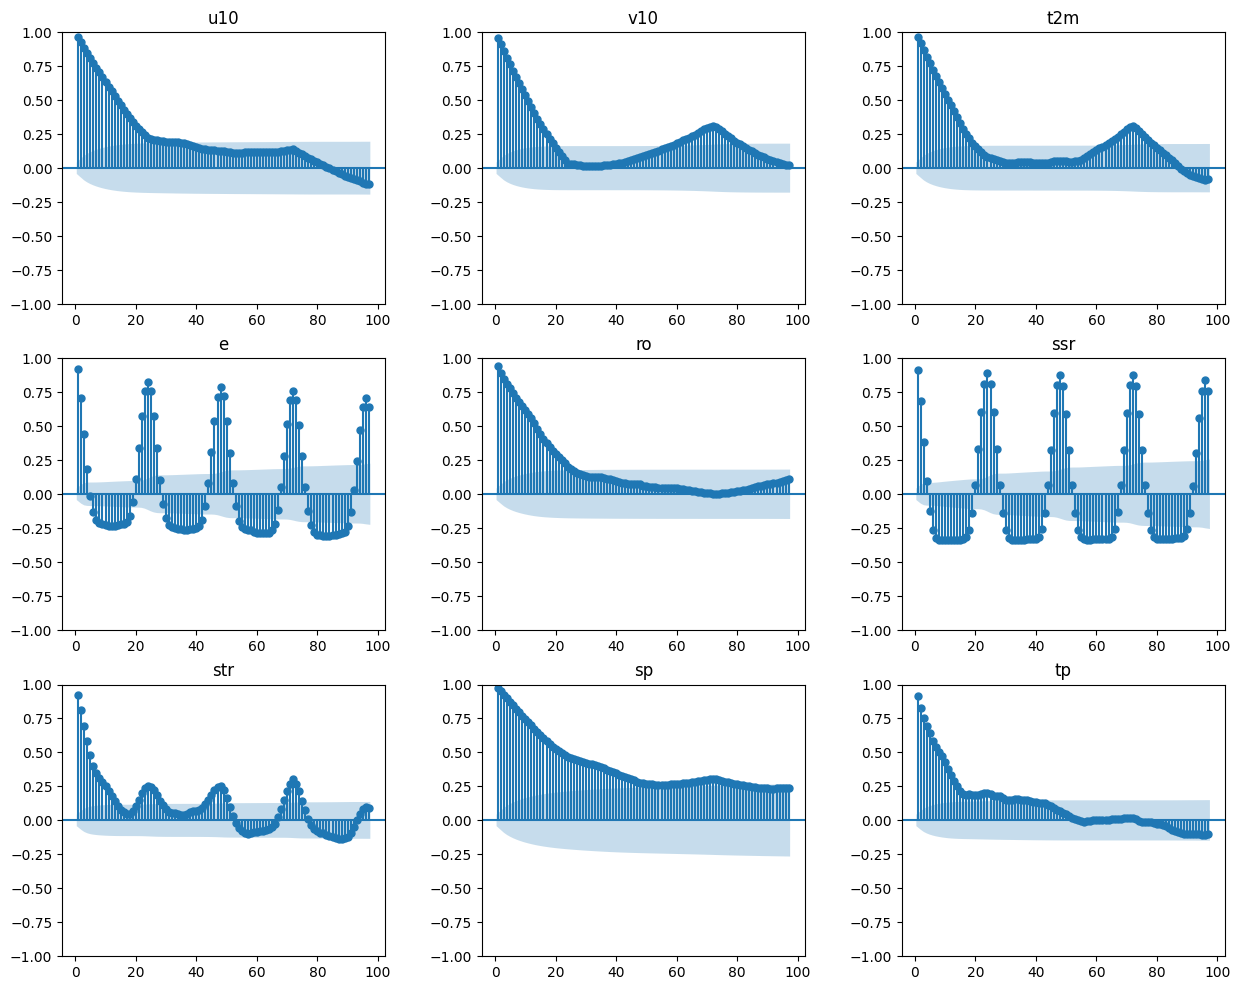
\includegraphics[width=\textwidth]{images/dt_autocorr.png}
    \caption{Współczynnik autokorelacji dla drzewa decyzyjnego dla wartości przesunięcia w zakresie czterech dni}
    \label{dt-autocorr}
\end{figure}

W przypadku drzewa decyzyjnego, dla którego autokorelacja została ukazana na wykresie \ref{dt-autocorr},
wygenerowane wykresy pokazują o wiele bardziej losową naturę. Nagłe skoki nie podążają za dziennymi cyklami,
co może wskazywać na "ślepe" powtarzanie wcześniej zaobserwowanych pomiarów. 

\begin{figure}[H]
    \centering
    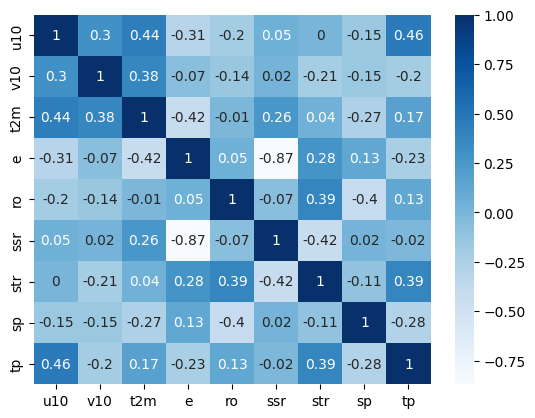
\includegraphics[width=\textwidth]{images/svr_corr_matrix.png}
    \caption{Korelacja pomiędzy parametrami w stworzonych prognozach dla algorytmu SVR}
    \label{svr-corr-matrix}
\end{figure}

Na powyższym rysunku \ref{svr-corr-matrix} pokazana została korelacja pomiędzy poszczególnymi atrybutami.
Pokazane wartości są bliskie w wartości do podobnej analizy przeprowadzonej dla danych pomiarowych. 
Największa korelacja istnieje pomiędzy promieniowaniem słonecznym a odparowaniem i wynosi -0,87 (-0,63 dla
rzeczywistego zbioru). Poza tym brak bardziej znaczących wartości z pominięciem tp-str, str-ssr i temperaturą
względem prędkości wiatru. Jednym z odchyleń względem rzeczywistości zdaje się wysoka wartość dla 
relacji między ciśnieniem atmosferycznym a odpływem cieków wodnych, która nie występuję w naturze.

\begin{figure}[H]
    \centering
    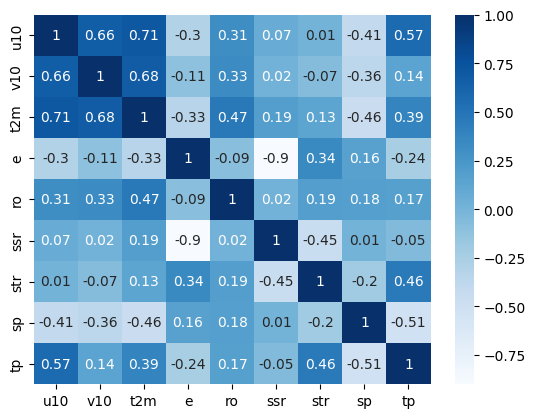
\includegraphics[width=\textwidth]{images/dt_corr_matrix.png}
    \caption{Korelacja pomiędzy parametrami w stworzonych prognozach dla drzewa decyzyjnego}
    \label{dt-corr-matrix}
\end{figure}

Taki sam wykres został stworzony dla drzewa decyzyjnego na rysunku \ref{dt-corr-matrix}. Możemy na nim 
zaobserwować podobne wzorce, lecz z o wiele większą korelacją pomiędzy poszczególnymi atrybutami. 
Wartości korelacji sięgają wartości od $-0,9$ aż do $0,71$. Algorytm drzewa decyzyjnego zdaje się 
bazować swoje wyniki bezpośrednio na relacjach występujących pomiędzy pojedynczymi atrybutami,
a w rezultacie ignorując głębsze zależności występujące w danych.


% Tables and figures: Present your data in tables and figures 
% that are clear, concise, and easy to read. Ensure that your 
% tables and figures are properly labeled and that they effectively 
% illustrate your findings.

% Subgroup analyses: Conduct subgroup analyses if relevant to 
% your research questions. For example, if you are comparing the 
% performance of different machine learning models, you might conduct 
% subgroup analyses based on the type of model used or the size of the training data.
\subsection{Porównanie modeli}

\begin{figure}[H]
    \centering
    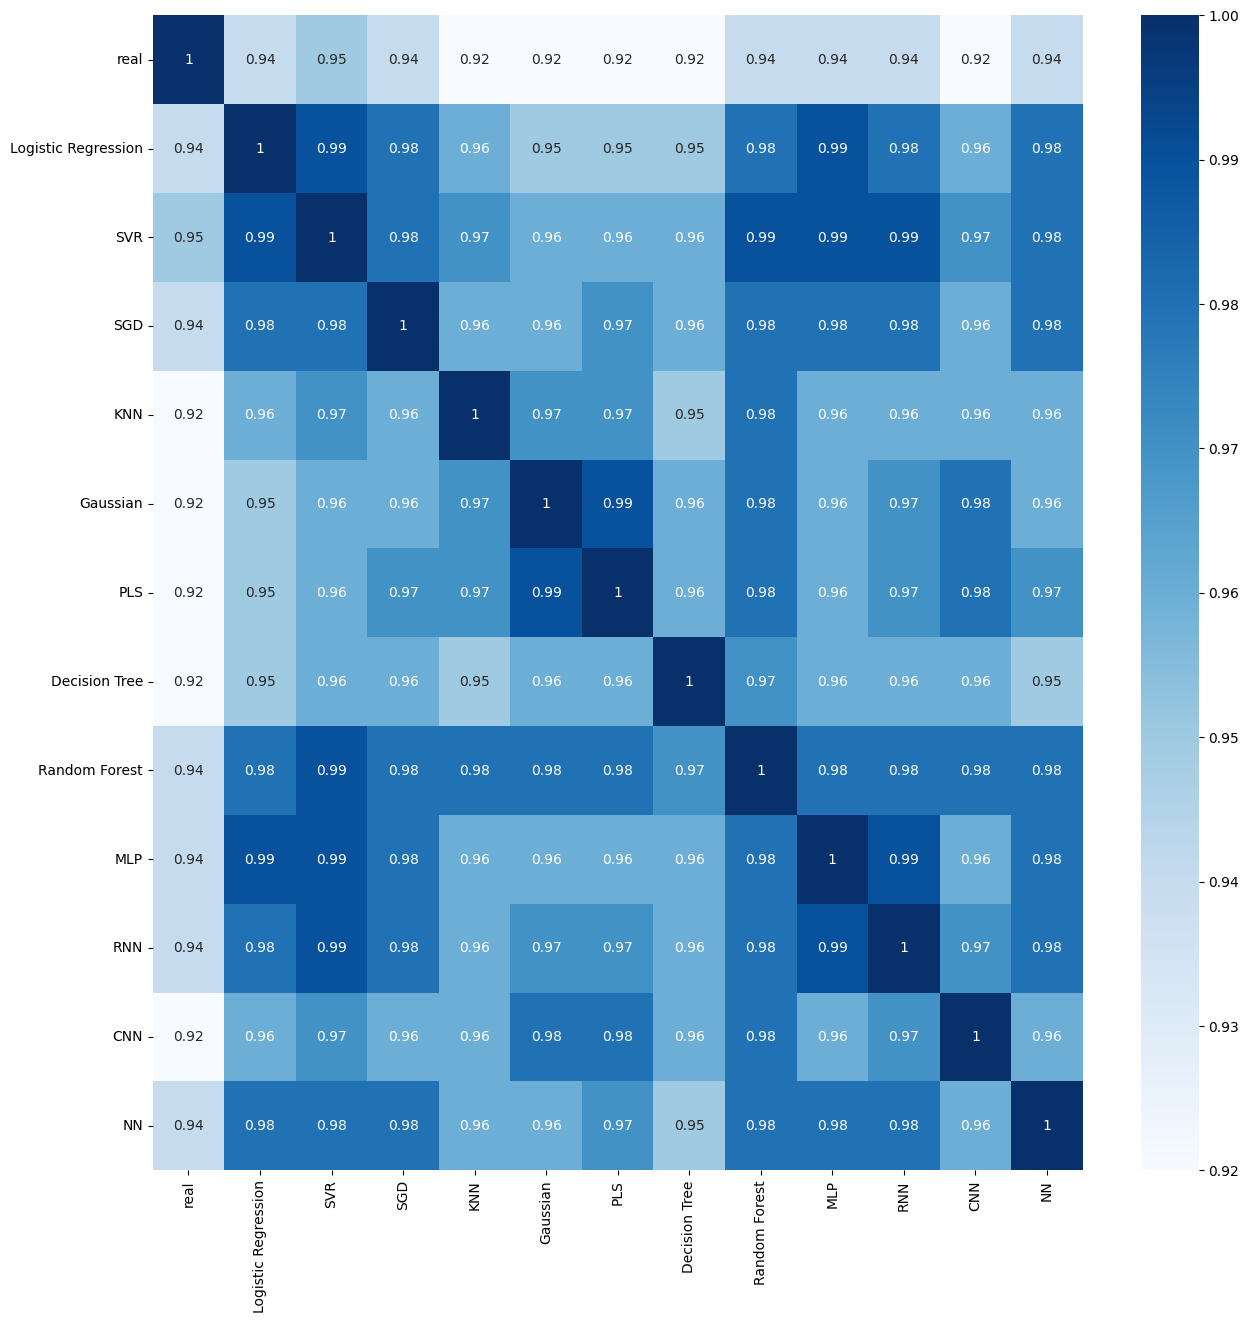
\includegraphics[width=\textwidth]{images/pred_corr.png}
    \caption{Korelacja pomiędzy wynikami stworzonymi poprzez poszczególne modele}
    \label{pred_corr}
\end{figure}

Porównując modele, można zastosować te same metryki jak w przypadku ewaluacji predykcji względem 
danych rzeczywistych. Największe wartości korelacji są widoczne pomiędzy modelami SVR, regresji logistycznej,
lasu losowego, MLP i RNN. Są to wszystkie modele, które w przeprowadzonych eksperymentach uzyskały najlepsze
rezultaty. Kolejną grupą algorytmów znajdujących się blisko siebie jest regresja gaussowska, PLS oraz CNN,
które, chociaż nie uzyskały najlepszych rezultatów, znajdowały się wśród algorytmów o średniej wydajności.
Drzewo decyzyjne będące przykładem najgorszego z rozważanych algorytmów znajduję się w dużej odległości
od pozostałych modeli.

Podobną analizę można przeprowadzić również ze względu na wartość błędu absolutnego i średniokwadratowego,
czego wyniki zostały zobrazowane na rysunku \ref{mse-matrix} oraz \ref{mae-matrix}.

\begin{figure}[H]
    \centering
    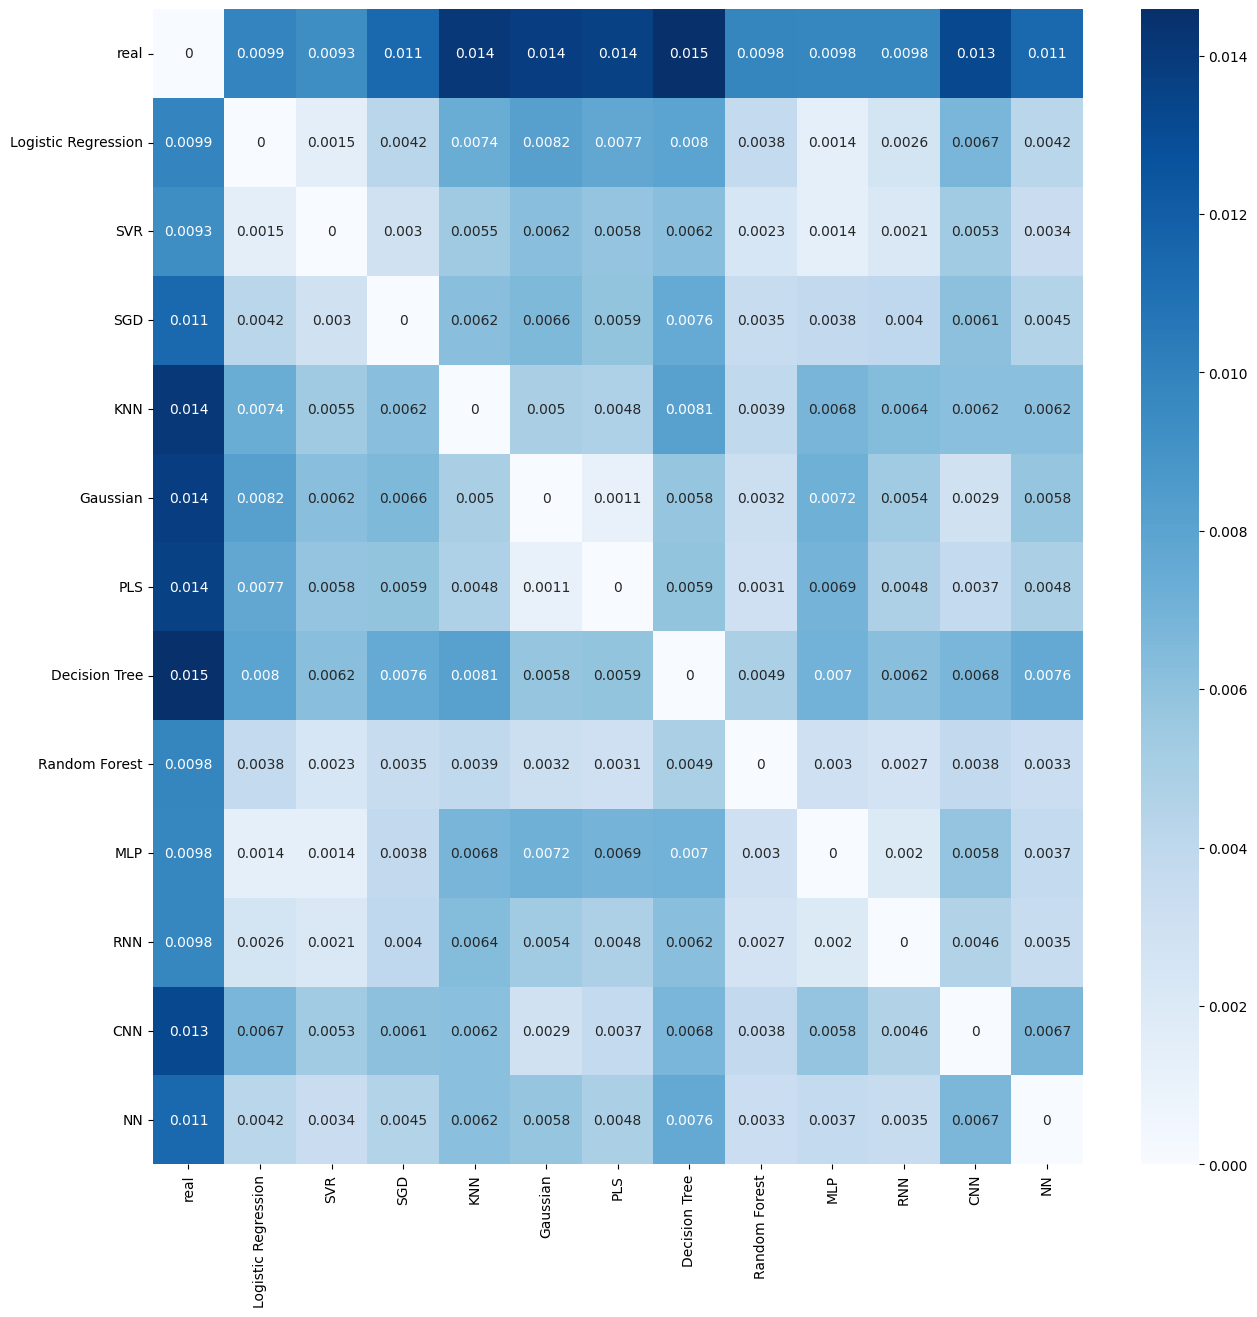
\includegraphics[width=\textwidth]{images/mse_matrix.png}
    \caption{Wartość błędu średniokwadratowego pomiędzy wynikami stworzonymi poprzez poszczególne modele}
    \label{mse-matrix}
\end{figure}

\begin{figure}[H]
    \centering
    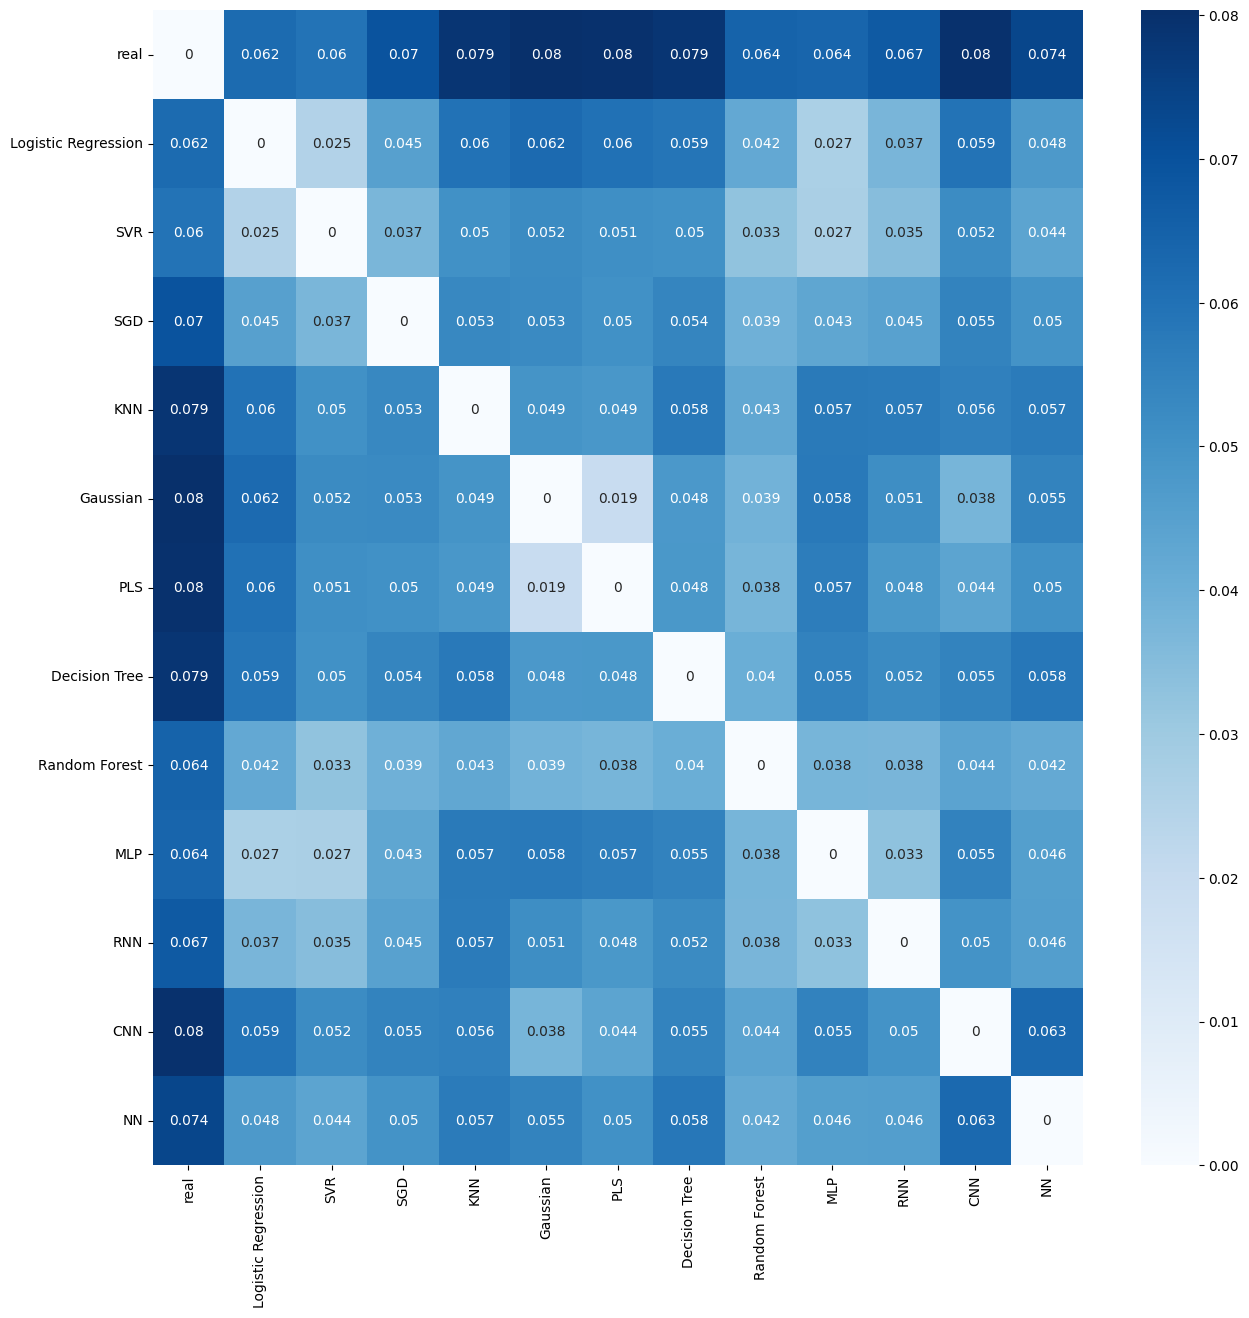
\includegraphics[width=\textwidth]{images/mae_matrix.png}
    \caption{Wartość średniego błędu absolutnego pomiędzy wynikami stworzonymi poprzez poszczególne modele}
    \label{mae-matrix}
\end{figure}

Wszystkie metryki wskazują na podobne rozdysponowanie rozważanych modeli względem siebie. Warto również wskazać
fakt, że wartość błędu większości modeli względem siebie nie przekraczała wartości błędu względem wartości
referencyjnych.

% \begin{figure}[H]
%     \centering
%     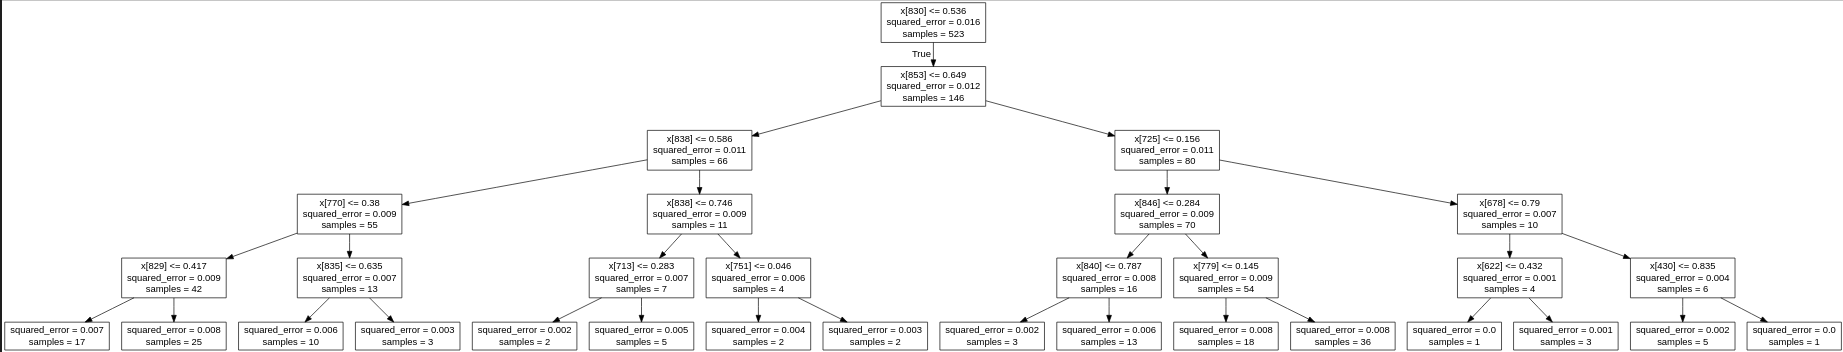
\includegraphics[width=\textwidth]{images/tree.png}
%     \caption{}
%     \label{tree-graph}
% \end{figure}

% Interpretation: Provide an interpretation of your findings and 
% relate them back to your research questions or hypotheses. Discuss 
% the implications of your results for the broader field of weather 
% prediction and the use of artificial intelligence and machine learning 
% techniques in this area.
% \subsection{Interpretacja}

% Limitations: Discuss any limitations of your study that may 
% have affected the validity or generalizability of your findings. 
% Be sure to acknowledge any potential sources of bias or confounding variables.
\subsection{Ograniczenia i możliwy rozwój}

Pierwszym ograniczeniem, którym warto wspomnieć podczas analizy otrzymanych wyników, jest 
mała liczba zasobów obliczeniowych w celu przeprowadzenia badań. Większe możliwości pozwoliłyby
na sprawdzenie większych modeli oraz walidację większej ilości hiperparametrów. Co więcej, 
chociaż dane godzinne zebrane z dwudziestu miesięcy reprezentują dość duże obciążenie
w obróbce i przetwarzaniu, to trening zaawansowanych modeli wymagałby o wiele większej liczby 
obserwacji i parametrów uwzględnionych w zbiorze danych.

Co więcej, przeprowadzone badania uwzględniały tylko jedną lokalizację w przeprowadzonej regresji,
a wpływ zjawisk globalnych został zignorowany. W dalszych analizach potrzeba by było przeanalizować
obserwacje pogodowe pochodzące z całego regionu, co znacznie powiększyłoby wymiar danych wejściowych
i przedłużyłoby proces uczenia i testowania.

Możliwym ulepszeniem wartym rozważenia w przyszłych badaniach jest zastosowanie bardziej zaawansowanych
architektur sieci neuronowych. W niniejszej pracy rozważone zostały sieci konwolucyjne i rekurencyjne.
Możliwe byłoby zastosowanie podejść hybrydowych o większej liczbie warstw ukrytych. Innym sposobem
byłoby także zastosowanie wcześniej wytrenowanych sieci w celu użycia uczenia transferowego i utylizacji
już nabytej wiedzy.

Ponadto, użyty zbiór danych składał się z wcześniej przetworzonych danych i niekoniecznie idealnie
odwzorowywał rzeczywiste zachowanie warunków pogodowych. Zbiór ERA5 jest zbiorem reanalysis i choć
zawiera kompleksowy zbiór parametrów i dużą rozdzielczość, to jest zależny od dokładności pomiarowej
urządzeń użytych do badania atmosfery. Algorytmy syntezy danych użyte w celu interpolacji otrzymanych
pomiarów do siatki modelowanej przez metody numeryczne także wnoszą pewien stopień błędu.




% % Discuss the significance of the results obtained and their implications 
% for the field of weather prediction. Identify the strengths and limitations 
% of the methodology and the algorithms used, and suggest areas for future research.

% The discussion section of your thesis is where you 
% interpret and explain the results of your study, and discuss 
% their implications for your research questions or hypotheses. Here are some 
% important elements to consider including in your discussion section:

% Summary of results: Provide a brief summary of your results, highlighting 
% the key findings and their statistical significance.

% Comparison to previous research: Compare your results to previous research 
% in the field. Discuss how your findings are similar or different from those 
% reported in the literature, and explain any discrepancies or inconsistencies.

% Interpretation of results: Provide an interpretation of your results in 
% light of your research questions or hypotheses. Discuss what the results 
% mean in terms of the broader field of weather prediction and the use of 
% artificial intelligence and machine learning techniques in this area.

% Implications and applications: Discuss the implications of your findings 
% for practice, policy, or future research. Explain how your results can be 
% applied to improve weather prediction or inform decision-making in this area.

% Limitations and recommendations for future research: Discuss any limitations 
% of your study that may have affected the validity or generalizability of your 
% findings, and provide recommendations for future research. Explain how future 
% research can build on your study to further advance our understanding of the 
% application of artificial intelligence and machine learning in weather prediction.

% Conclusion: Provide a brief summary of the main findings of your study 
% and their implications, and emphasize the contribution that your study 
% has made to the broader field of weather prediction.

% Overall, the discussion section of your thesis should provide a thoughtful 
% and detailed interpretation of your results, and highlight their implications 
% for practice, policy, or future research.
\section{Analiza wyników}
% Summarize the key findings of your research and restate the thesis statement.

% If some of the models you tested didn't work well, it's important to 
% acknowledge this in your thesis and discuss the reasons why these models 
% failed to perform as expected. Here are some suggestions for how to 
% approach this in your writing:

% Discuss the limitations of the models: Explain any limitations 
% of the models that may have impacted their performance. This could 
% include issues related to data quality or quantity, inappropriate 
% algorithmic choices, or parameter settings.

\section{Wnioski}

% Provide a critical analysis: Provide a critical analysis of the models 
% that did not perform well, highlighting both their strengths and limitations. 
% Be honest and transparent about the performance of these models, and 
% explain how this impacts the overall results of your research.
\subsection{Analiza wyników}

% Identify areas for improvement: Based on your analysis of the models, 
% identify areas where improvements could be made in future research. 
% This could include exploring different algorithms, feature engineering, 
% or using alternative data sources.
\subsection{Możliwości poprawy}

% Discuss the implications for your research: Discuss the implications 
% of the poor performance of some of the models for your research question 
% and the field of weather prediction in general. Consider how these 
% results may impact future research or the practical applications 
% of these techniques.
\subsection{Wpływ przeprowadzonych badań}

\section*{Skróty}

\raggedright{}

AI — sztuczna inteligencja

DL — uczenie głębokie

ML — uczenie maszynowe

NWP — numeryczne prognozowanie pogody

GAN — generative adversarial network

ECMWF — Europejskie Centrum Średnioterminowych Prognoz Pogody

MSE — błąd średniokwadratowy

RMSE — pierwiastek błędu średniokwadratowego

MAE — błąd absolutny

IoT — internet rzeczy

MOS — statystyki wyjścia modelu

PCA — analiza głównych składowych

MLP — perceptron wielowarstwowy

RNN — rekurencyjna sieć neuronowa

CNN — konwolucyjna sieć neuronowa

LSTM — long-short term memory

GRU — gated recurrent unit

C3S — Copernicus Climate Change Service

UCAR — University Corporation for Atmospheric Research

CORR — współczynnik korelacji

\pagebreak
\printbibliography[title={Bibliografia}]
% \section*{Appendix}

\begin{lstlisting}[label=python-listing,caption={Kod źródłowy},language=python]
import xarray as xr
import pandas as pd

ds = xr.open_dataset('/content/drive/My Drive/era5/era5_03-19.nc', 
    engine='netcdf4')
ds2 = xr.open_dataset('/content/drive/My Drive/era5/era5_20-22.nc', 
    engine='netcdf4')
df = ds.to_dataframe()
df2 = ds2.to_dataframe()

df

df.describe()

df.isna().any()
empty_columns=[]

for i in list(df.columns):
    empty_values = df[i].isnull().sum()
    if empty_values > 0:
        print(i, empty_values, empty_values / df.shape[0])

df.index

# df.loc[24.0, 49.0]
df.loc[18.899999618530273, 49.900001525878906]

df.loc[:,:,"2018-01-01 00:00:00"]

"""## Nan handling"""

df.interpolate(inplace=True)
df2.interpolate(inplace=True)
for column in df.columns:
    df[column].fillna(df[column].mean(), inplace=True)
    df2[column].fillna(df2[column].mean(), inplace=True)


for i in list(df.columns):
    empty_values = df[i].isnull().sum()
    if empty_values > 0:
        print(i, empty_values, empty_values / df.shape[0])

"""## Plots"""

df = pd.concat([df, df2])
df

from statsmodels.graphics import tsaplots
import matplotlib.pyplot as plt
import matplotlib.pyplot as plt
from math import ceil, sqrt

n = ceil(sqrt(len(df.columns)))
f, a = plt.subplots(n, n, figsize=(15, 12))
for column, ax in zip(df.columns, a.ravel()):
    plot = tsaplots.plot_acf(df[column], lags=range(1, 98), ax=ax)
    ax.set_title(column)
plt.subplots_adjust(wspace=.3)

fig, ax = plt.subplots()
lag = 24
plt.scatter(df["t2m"][:-lag], df["t2m"][lag:], 
    c=range(len(df)-lag), s=2)
ax.set_xlabel("Temperatura [K]")
ax.set_ylabel("Temperatura [K]")

fig, ax = plt.subplots()
lag = 24
length = 200
plt.plot(df["t2m"][:length], df["t2m"][lag:lag+length])
ax.set_xlabel("Temperatura [K]")
ax.set_ylabel("Temperatura [K]")

fig, ax = plt.subplots()
lag = 24
plt.scatter(df["sp"][:-lag], df["sp"][lag:], c=range(len(df)-lag), s=2)
ax.set_xlabel("Cisnienie [Pa]")
ax.set_ylabel("Cisnienie [Pa]")

import matplotlib.pyplot as plt
fix, ax = plt.subplots()
plt.scatter(df["ssr"], df["e"], c = range(len(df)), s=2)
ax.set_xlabel("Promieniowanie sloneczne [J/m^2]")
ax.set_ylabel("Odpwarowanie [m]")

fig, ax = plt.subplots()
lag = 24
plt.scatter(df["tp"][:-lag], df["tp"][lag:], c=range(len(df)-lag), s=2)
ax.set_xlabel("Opady [m]")
ax.set_ylabel("Opady [m]")

n = ceil(sqrt(len(df.columns)))
f, a = plt.subplots(n, n, figsize=(12, 12))
lag = 24
for column, ax in zip(df.columns, a.ravel()):
    ax.hexbin(df[column][:-lag], df[column][lag:], gridsize=40)
    ax.set_title(column)

plt.subplots_adjust(wspace=.3)
plt.subplots_adjust(hspace=.3)

a[1][0].set_xticklabels(a[1][0].get_xticklabels(), rotation=15, ha='center')
a[2][0].set_xticklabels(a[2][0].get_xticklabels(), rotation=15, ha='center')
a[2][1].set_xticklabels(a[2][1].get_xticklabels(), rotation=15, ha='center')
a[2][2].set_xticklabels(a[2][2].get_xticklabels(), rotation=15, ha='center')

import pandas as pd
import seaborn as sns
import matplotlib.pyplot as plt

matrix = df.corr().round(2)
sns.heatmap(matrix, annot=True, cmap="Blues")
plt.show()

import math
import numpy as np
from scipy.stats import lognorm
import statsmodels.api as sm
import matplotlib.pyplot as plt
import matplotlib.pyplot as plt
from math import ceil, sqrt

n = ceil(sqrt(len(df.columns)))
f, a = plt.subplots(n, n, figsize=(15, 12))
for column, ax in zip(df.columns, a.ravel()):
    plot = sm.qqplot(df[column], ax=ax)
    ax.set_title(column)
    ax.set_xlabel("")
    ax.set_ylabel("")
    
plt.subplots_adjust(wspace=.3)

from scipy.stats import shapiro 
from scipy.stats import lognorm
from scipy.stats import kstest
from scipy.stats import normaltest

#that's just blatant lies
for column in df.columns:
    print(column + "  " + str(normaltest(df[column]).pvalue))

import matplotlib.pyplot as plt
from math import ceil, sqrt

n = ceil(sqrt(len(df.columns)))
f, a = plt.subplots(n, n, figsize=(15, 12))
for column, ax in zip(df.columns, a.ravel()):
    plot = df.boxplot(column=column, ax=ax, figsize=(30, 30))
plt.subplots_adjust(wspace=.3)

plot = df.hist(bins=20, figsize=(12, 12))
plot[1][0].set_xticklabels(plot[1][0].get_xticklabels(), 
    rotation=15, ha='center')
plot[2][0].set_xticklabels(plot[2][0].get_xticklabels(), 
    rotation=15, ha='center')
plot[2][1].set_xticklabels(plot[2][1].get_xticklabels(), 
    rotation=15, ha='center')
plot[2][2].set_xticklabels(plot[2][2].get_xticklabels(), 
    rotation=15, ha='center')

import matplotlib.pyplot as plt
from math import ceil, sqrt

timeframe = 3000

n = ceil(sqrt(len(df.columns)))
f, a = plt.subplots(n, n, figsize=(12, 12))
for column, ax in zip(df.columns, a.ravel()):
    plot = df[column][:timeframe].rolling(window=92)
        .mean().plot(ax=ax)
    ax.set_xticklabels([])
    ax.set_xlabel("time")
    ax.set_title(column)
plt.subplots_adjust(wspace=.3)

"""## Scaling"""

from sklearn.preprocessing import StandardScaler, MinMaxScaler
import numpy as np
from joblib import dump, load

scaler = MinMaxScaler()

df[df.columns] = scaler.fit_transform(df[df.columns])
df2[df2.columns] = scaler.transform(df2[df2.columns])

df.head()

dump(scaler, '/content/drive/My Drive/era5/standard_scaler.bin', 
    compress=True)
df.to_csv('/content/drive/My Drive/era5/weather.csv', 
    compression="gzip")
df2.to_csv('/content/drive/My Drive/era5/weather2.csv', 
    compression="gzip")

"""# Classification

## Data reading
"""

import pandas as pd
from tensorflow.keras.preprocessing import timeseries_dataset_from_array
import numpy as np

def prepare_single_location_data(test=False, additional=False):
    if test:
        df = pd.read_csv('/content/drive/My Drive/era5/weather2.csv', 
            compression='gzip', index_col=[0, 1, 2])
    elif(additional==False):
        df = pd.read_csv('/content/drive/My Drive/era5/weather.csv', 
            compression='gzip', index_col=[0, 1, 2])
    else:
        df = pd.read_csv('/content/drive/My Drive/era5/weather3.csv', 
            compression='gzip', index_col=[0, 1, 2])
        df = df.to_numpy()
        X = timeseries_dataset_from_array(df, None, sequence_length=96, 
            sequence_stride=24, sampling_rate=1, start_index=0, end_index=len(df)-24, batch_size=None)
        y = timeseries_dataset_from_array(df, None, sequence_length=24, 
            sequence_stride=24, sampling_rate=1, start_index=96, batch_size=None)
    return X, y

from google.colab import drive
drive.mount('/content/drive')

X, y = prepare_single_location_data()
X, y = np.array(list(X)), np.array(list(y))

X_test, y_test = prepare_single_location_data(True)
X_test, y_test = np.array(list(X_test)), np.array(list(y_test))

"""## Neural networks"""

from keras.engine import input_layer
from sklearn.base import BaseEstimator
from keras.models import Sequential 
from keras.layers import Dense 
from keras.layers import GRU
from keras.layers import Concatenate, Reshape, Conv2D, 
    MaxPooling2D, Flatten
from keras import Input, Model
from sklearn.metrics import mean_squared_error, mean_absolute_error
from keras.callbacks import EarlyStopping, ModelCheckpoint

class RNN(BaseEstimator):
    def __init__(self, epochs=10, layer1=[16, 16], layer2=[16, 16], 
        loss="mean_squared_error", optimizer="adam", metrics="MSE"):
    self._estimator_type = "regressor"
    self.epochs = epochs
    self.layer1 = layer1
    self.layer2 = layer2
    self.loss = loss
    self.optimizer = optimizer
    self.metrics = metrics

    def fit(self, X, y, params=None):
    if params == None:
        params = {
            "epochs": self.epochs,
            "layer1": self.layer1,
            "layer2": self.layer2,
            "loss": self.loss,
            "optimizer": self.optimizer,
            "metrics": self.metrics
        }

    n_epochs = params["epochs"] or self.epochs
    n_layer1 = params["layer1"] or self.layer1
    n_layer2 = params["layer2"] or self.layer2
    loss_function = params["loss"] or "mean_squared_error"
    optimizer_function = params["optimizer"] or "adam"
    metrics = params["metrics"] or "MSE"

    input = Input(shape=(X.shape[1], X.shape[2]))

    x = GRU(n_layer1[0], return_sequences=True)(input)
    for n_layer in n_layer1[1:]:
        x = GRU(n_layer, return_sequences=True)(x)
    x = Flatten()(x)
    for n_layer in n_layer2:
        x = Dense(n_layer)(x)
    x = Dense(y.shape[1])(x)

    output = x

    self.model = Model(inputs=[input], outputs=[output])
    self.model.compile(loss=loss_function, optimizer=optimizer_function, 
        metrics=metrics) 
    self.model.build(input_shape=(X.shape[1], X.shape[2]))

    self.model.fit(X, y, epochs=n_epochs, batch_size=1, verbose=0)
    return self

    def predict(self, X):
    y = self.model.predict(X)
    return y

    def save(self, path):
    self.model.save(path)

    def score(self, X, y):
    return mean_squared_error(self.predict(X), y)

    def get_params(self, deep=True):
    return {
            "epochs": self.epochs,
            "layer1": self.layer1,
            "layer2": self.layer2,
            "loss": self.loss,
            "optimizer": self.optimizer,
            "metrics": self.metrics
        }

from keras.engine import input_layer
from sklearn.base import BaseEstimator
from keras.models import Sequential 
from keras.layers import Dense 
from keras.layers import GRU
from keras.layers import Concatenate, Reshape, Conv2D, 
    MaxPooling2D, Flatten
from keras import Input, Model
from sklearn.metrics import mean_squared_error, mean_absolute_error

class CNN(BaseEstimator):
    def __init__(self, epochs=10, layer1=[16, 16], layer2=[16, 16], 
        loss="mean_squared_error", optimizer="adam", metrics="MSE"):
    self._estimator_type = "regressor"
    self.epochs = epochs
    self.layer1 = layer1
    self.layer2 = layer2
    self.loss = loss
    self.optimizer = optimizer
    self.metrics = metrics

    def fit(self, X, y, params=None):
    if params == None:
        params = {
            "epochs": self.epochs,
            "layer1": self.layer1,
            "layer2": self.layer2,
            "loss": self.loss,
            "optimizer": self.optimizer,
            "metrics": self.metrics
        }

    n_epochs = params["epochs"] or self.epochs
    n_layer1 = params["layer1"] or self.layer1
    n_layer2 = params["layer2"] or 16
    loss_function = params["loss"] or "mean_squared_error"
    optimizer_function = params["optimizer"] or "adam"
    metrics = params["metrics"] or "MSE"

    input = Input(shape=(X.shape[1], X.shape[2]))

    x = Reshape((96, 9, 1))(input)

    x = Conv2D(n_layer1[0], (3, 3), input_shape=(96, 9, 1))(x)

    for n_layer in n_layer1[1:]:
        x = Conv2D(n_layer, (3, 3))(x)

    x = Flatten()(x)

    for n_layer in n_layer2:
        x = Dense(n_layer)(x)
        x = Dense(n_layer)(x)
    x = Dense(y.shape[1])(x)

    output = x

    self.model = Model(inputs=[input], outputs=[output])
    self.model.compile(loss=loss_function, optimizer=optimizer_function, 
        metrics=metrics) 
    self.model.build(input_shape=(X.shape[1], X.shape[2]))
    self.model.fit(X, y, epochs=n_epochs, batch_size=1, verbose=0)
    return self

    def predict(self, X):
    y = self.model.predict(X)
    return y

    def save(self, path):
    self.model.save(path)

    def score(self, X, y):
    return mean_squared_error(self.predict(X), y)

    def get_params(self, deep=True):
    return {
            "epochs": self.epochs,
            "layer1": self.layer1,
            "layer2": self.layer2,
            "loss": self.loss,
            "optimizer": self.optimizer,
            "metrics": self.metrics
        }

from keras.engine import input_layer
from sklearn.base import BaseEstimator
from keras.models import Sequential 
from keras.layers import Dense 
from keras.layers import GRU
from keras.layers import Concatenate, Reshape, Conv2D, 
    MaxPooling2D, Flatten
from keras import Input, Model
from sklearn.metrics import mean_squared_error, mean_absolute_error

class NN(BaseEstimator):
    def __init__(self, epochs=10, layer1=[16, 16], loss="mean_squared_error", 
        optimizer="adam", metrics="MSE"):
    self._estimator_type = "regressor"
    self.epochs = epochs
    self.layer1 = layer1
    self.loss = loss
    self.optimizer = optimizer
    self.metrics = metrics

    def fit(self, X, y, params=None):
    if params == None:
        params = {
            "epochs": self.epochs,
            "layer1": self.layer1,
            "loss": self.loss,
            "optimizer": self.optimizer,
            "metrics": self.metrics
        }

    n_epochs = params["epochs"] or self.epochs
    n_layer1 = params["layer1"] or self.layer1
    loss_function = params["loss"] or "mean_squared_error"
    optimizer_function = params["optimizer"] or "adam"
    metrics = params["metrics"] or "MSE"

    input = Input(shape=(X.shape[1], X.shape[2]))

    x = Flatten()(input)

    for n_layer in n_layer1:
        x = Dense(n_layer)(x)
    x = Dense(y.shape[1])(x)

    output = x

    self.model = Model(inputs=[input], outputs=[output])
    self.model.compile(loss=loss_function, optimizer=optimizer_function, 
        metrics=metrics) 
    self.model.build(input_shape=(X.shape[1], X.shape[2]))
    self.model.fit(X, y, epochs=n_epochs, batch_size=1, verbose=0)
    return self

    def predict(self, X):
    y = self.model.predict(X)
    return y

    def save(self, path):
    self.model.save(path)

    def score(self, X, y):
    return mean_squared_error(self.predict(X), y)

    def get_params(self, deep=True):
    return {
            "epochs": self.epochs,
            "layer1": self.layer1,
            "loss": self.loss,
            "optimizer": self.optimizer,
            "metrics": self.metrics
        }

"""## Voting"""

from sklearn.base import BaseEstimator, TransformerMixin

class Reshaper(BaseEstimator, TransformerMixin):
    def fit(self, X, y=None):
    return self
    
    def transform(self, X, y=None):
    shape = X.shape
    return X.reshape(shape[0], shape[1] * shape[2])

import numpy as np
from sklearn.preprocessing import normalize

class MultioutputVotingRegressor(BaseEstimator):
    def __init__(self, estimators, filter, weights=None):
    self.estimators = estimators
    self.filter = filter
    if weights == None:
        self.weights = [1. / len(self.filter)] * len(self.filter)
    else:
        self.weights = weights

    def fit(self, X, y=None):
    for weight, name in self.weights, self.estimators:
        if name in self.filter:
        weight = 1. / self.estimators[name].score(X, y)
    self.weights = normalize(self.weights)

    def predict(self, X):
    results = []
    for name in self.estimators:
        if name in self.filter:
        results.append(self.estimators[name].predict(X))
    return np.average(results, axis=0, weights=self.weights)
    
    def score(self, X, y):
    return mean_squared_error(self.predict(X), y)
    
    def transform(self, X, y=None):
    return self.predict(X)

"""## Classification"""

from sklearn.experimental import enable_halving_search_cv 
from sklearn import tree, svm, linear_model, neighbors, 
    gaussian_process, cross_decomposition, ensemble, neural_network
from sklearn.multioutput import MultiOutputRegressor
from sklearn.metrics import mean_squared_error, mean_absolute_error
from sklearn.pipeline import Pipeline
from sklearn.decomposition import PCA
from sklearn.preprocessing import StandardScaler
from sklearn.model_selection import GridSearchCV, RandomizedSearchCV, HalvingGridSearchCV
import pandas as pd
from joblib import dump, load
from os import path
from keras.models import load_model
from matplotlib import pyplot as plt
import numpy as np
import warnings

warnings.filterwarnings("ignore")


df = pd.DataFrame()
individual_scores = [pd.DataFrame() for i in range(9)]


clfs = {
    "Logistic Regression": Pipeline([('reshaper', Reshaper()), ('clf', MultiOutputRegressor(GridSearchCV(linear_model.Ridge(), {"solver": ('svd', 'cholesky', 'lsqr', 'sparse_cg', 'sag', 'saga', 'lbfgs')})))]),
    "SVR": Pipeline([('reshaper', Reshaper()), 
        ("clf", MultiOutputRegressor(GridSearchCV(svm.SVR(), 
            {"kernel": ('linear', 'poly', 'rbf', 'sigmoid'), 
            "C": (0.1, 1., 10), "epsilon": (0.01, 0.1, 1)})))]),
    "SGD": Pipeline([('reshaper', Reshaper()), 
        ('clf', MultiOutputRegressor(GridSearchCV(linear_model.SGDRegressor(), 
            {"penalty": ('l2', 'l1', 'elasticnet'), 
            "loss": ('squared_error', 'huber', 'epsilon_insensitive', 'squared_epsilon_insensitive')})))]),
    "KNN": Pipeline([('reshaper', Reshaper()), ('clf', GridSearchCV(neighbors.KNeighborsRegressor(), {"weights": ("unifor", "distance"), "algorithm": ('ball_tree', 'kd_tree', 'brute'), "p": (1, 2, 3, 4)}))]),
    "Gaussian": Pipeline([('reshaper', Reshaper()), ('clf', GridSearchCV(gaussian_process.GaussianProcessRegressor(normalize_y=True), {"alpha": (1e-10, 1e-5, .01, .1), "n_restarts_optimizer": (0, 1, 2, 3, 4)}))]),
    "PLS": Pipeline([('reshaper', Reshaper()), ('clf', cross_decomposition.PLSRegression())]),
    "Decision Tree": Pipeline([('reshaper', Reshaper()), ('clf', GridSearchCV(tree.DecisionTreeRegressor(), {"splitter": ("best", "random"), "min_samples_leaf": (1, 2, 3, 4), "max_depth": (None, 5, 10, 15, 20)}))]),
    "Random Forest": Pipeline([('reshaper', Reshaper()), ('clf', ensemble.RandomForestRegressor())]),
    "MLP": Pipeline([('reshaper', Reshaper()), ('clf', GridSearchCV(neural_network.MLPRegressor(), {'activation': ('identity', 'logistic', 'tanh', 'relu'), "solver": ('lbfgs', 'sgd', 'adam')}))]),
    "RNN": HalvingGridSearchCV(RNN(), {"epochs": (10, 15), 
                                "layer1": (
                                    [32, 32],
                                    [32, 32, 32],
                                    [64, 32]
                                ), 
                                "layer2": (
                                    [32, 32],
                                    [32, 32, 32],
                                    [64, 32]
                                )}, cv=3, verbose=3),
    "CNN": HalvingGridSearchCV(CNN(), {"epochs": (10, 15, 20), 
                                "layer1": (
                                    [32, 32],
                                    [32, 32, 32],
                                    [64, 32],
                                    [64, 64, 64],
                                    [128, 128, 64]
                                ), 
                                "layer2": (
                                    [32, 32],
                                    [32, 32, 32],
                                    [64, 32],
                                    [64, 64, 64],
                                    [128, 128, 64]
                                )}, cv=3, verbose=3),
    "NN": HalvingGridSearchCV(NN(), {"epochs": (10, 15, 20), 
                                "layer1": (
                                    [32, 32],
                                    [32, 32, 32],
                                    [64, 32],
                                    [64, 64, 64],
                                    [128, 128, 64],
                                    [128, 128, 64, 32]
                                )}, cv=3, verbose=3)
}

voting = MultioutputVotingRegressor(estimators=clfs, filter=['SVR', 'Logistic Regression', 'SGD', 'PLS', 'Random Forest', 'MLP', 'RNN', 'CNN', 'NN'])

f, a = plt.subplots(12, 9, figsize=(50, 50))
n = 0

for name, clf in clfs.items():
    print(name)
    reshaper = Reshaper()
    y_learning, y_testing = reshaper.fit_transform(y), reshaper.fit_transform(y_test)

    filename = "/content/drive/My Drive/era5/classifiers/" + name

    if path.exists(filename):
    print("loaded")
    if name == "RNN" or name == "NN" or name == "CNN":
        clf = load_model(filename)
    else:
        clf = load(filename)
    clfs[name] = clf
    else:
    print("training")
    clf = clf.fit(X, y_learning)

    predicted_train = clf.predict(X)
    predicted_test = clf.predict(X_test)

    df = df.append({
        "Name": name,
        "MSE train": mean_squared_error(predicted_train, y_learning),
        "MAE train": mean_absolute_error(predicted_train, y_learning),
        "CORR train": np.corrcoef(predicted_train.flatten(), y_learning.flatten())[0][1],
        "MSE test": mean_squared_error(predicted_test, y_testing),
        "MAE test": mean_absolute_error(predicted_test, y_testing),
        "CORR test": np.corrcoef(predicted_test.flatten(), y_testing.flatten())[0][1]
    }, ignore_index=True)

    for i in range(9):
    individual_scores[i] = individual_scores[i].append({
        "Name": name,
        "MSE train": mean_squared_error(predicted_train[:][i::9], y_learning[:][i::9]),
        "MAE train": mean_absolute_error(predicted_train[:][i::9], y_learning[:][i::9]),
        "CORR train": np.corrcoef(predicted_train[:][i::9], y_learning[:][i::9]),
        "MSE test": mean_squared_error(predicted_test[:][i::9], y_testing[:][i::9]),
        "MAE test": mean_absolute_error(predicted_test[:][i::9], y_testing[:][i::9]),
        "CORR test": np.corrcoef(predicted_test[:][i::9], y_testing[:][i::9]),
    }, ignore_index=True)

    columns =["u10", "v10", "t2m", "e", "ro", "ssr", "str", "sp", "tp"]
    y_predicted = clf.predict(X_test)
    for i in range(9):
    a[n, i].set_title(name + " - " + columns[i])
    a[n, i].plot(y_predicted.flatten()[i::9])
    a[n, i].plot(y_testing.flatten()[i::9])
    n += 1
    try:
    print(clf[1].best_params_)
    except:
    print("exception")

    if not path.exists(filename) and (name == "RNN" or name == "NN" or name == "CNN"):
    clf.best_estimator_.save(filename)
    elif not path.exists(filename):
    dump(clf, filename)
    # clf.best_estimator_.save(filename)

# df = df.append({
#   "Name": "Ensemble",
#   "MSE train": mean_squared_error(voting.predict(X), y_learning),
#   "MAE train": mean_absolute_error(voting.predict(X), y_learning),
#   "CORR train": np.corrcoef(voting.predict(X), y_learning),
#   "MSE test": mean_squared_error(voting.predict(X_test), y_testing),
#   "MAE test": mean_absolute_error(voting.predict(X_test), y_testing),
#   "CORR test": np.corrcoef(voting.predict(X_test), y_testing)
# }, ignore_index=True)

df

import seaborn as sns

df = df.set_index("Name")
f, ax = plt.subplots(figsize=(5, 6))
sns.heatmap(df[["MSE train", "MSE test"]], annot=True, linewidths=.5, ax=ax, cmap="Blues")

import seaborn as sns

f, ax = plt.subplots(figsize=(5, 6))
sns.heatmap(df[["MAE train", "MAE test"]], annot=True, linewidths=.5, ax=ax, cmap="Blues")

import seaborn as sns

f, ax = plt.subplots(figsize=(5, 6))
sns.heatmap(df[["CORR train", "CORR test"]], annot=True, linewidths=.5, ax=ax, cmap="Blues")

f, a = plt.subplots(figsize=(10, 10))

df.sort_values('MSE test', inplace=True, ascending=False)
df.plot.barh(y='MSE test', ax=a)

f, a = plt.subplots(figsize=(10, 10))

df.sort_values('MAE test', inplace=True, ascending=False)
df.plot.barh(y='MAE test', ax=a)

f, a = plt.subplots(figsize=(10, 10))

df.sort_values('CORR test', inplace=True, ascending=True)
df.plot.barh(y='CORR test', ax=a)

X_test.shape

"""## Random day prediction"""

from random import randint

f, a = plt.subplots(12, 9, figsize=(50, 50))

day = randint(0, 88)

for n, name in enumerate(clfs):
    clf = clfs[name]
    y_predicted = clf.predict(X_test)[day]
    for i in range(9):
    a[n, i].set_title(name + " - " + columns[i])
    a[n, i].plot(y_predicted.flatten()[i::9])
    a[n, i].plot(y_testing[day].flatten()[i::9])

"""## Random week prediction"""

from random import randint
from sklearn.preprocessing import StandardScaler, MinMaxScaler
from joblib import dump, load
import pandas as pd


scaler = load('/content/drive/My Drive/era5/standard_scaler.bin')
scaler.feature_names_in_

f, a = plt.subplots(12, 9, figsize=(50, 50))

day = 21
print(day)

y_comparison = y_testing[day:day+7].reshape(168, 9)
y_comparison = scaler.inverse_transform(y_comparison)

for n, name in enumerate(clfs):
    clf = clfs[name]
    y_predicted = clf.predict(X_test)[day:day+7].reshape(168, 9)
    y_predicted = scaler.inverse_transform(y_predicted)

    df = pd.DataFrame(y_predicted)
    for i in range(9):
    a[n, i].set_title(name + " - " + columns[i])
    a[n, i].plot(y_predicted.flatten()[i::9])
    a[n, i].plot(y_comparison.flatten()[i::9])

f, a = plt.subplots(3, 3, figsize=(15, 12))
name = "Decision Tree"
clf = clfs[name]
y_predicted = clf.predict(X_test)[day:day+7].reshape(168, 9)
y_predicted = scaler.inverse_transform(y_predicted)
df = pd.DataFrame(y_predicted)
for i, ax in enumerate(a.ravel()):
    ax.set_title(name + " - " + columns[i])
    ax.plot(y_predicted.flatten()[i::9])
    ax.plot(y_comparison.flatten()[i::9])

import pandas as pd
import seaborn as sns
import matplotlib.pyplot as plt
from random import randint
from sklearn.preprocessing import StandardScaler, MinMaxScaler
from joblib import dump, load
import pandas as pd

df = pd.DataFrame()
df["real"] = pd.DataFrame(y_test.flatten())

for n, name in enumerate(clfs):
    clf = clfs[name]
    y_predicted = clf.predict(X_test).flatten()

    df[name] = pd.DataFrame(y_predicted)
# df

f, a = plt.subplots(figsize=(15, 15))
matrix = df.corr().round(2)
for name1 in df.columns:
    for name2 in df.columns:
    matrix[name1][name2] = mean_absolute_error(df[name1], df[name2])
sns.heatmap(matrix, annot=True, cmap="Blues")
plt.show()
# matrix

import math
import numpy as np
from scipy.stats import lognorm
import statsmodels.api as sm
import matplotlib.pyplot as plt
import matplotlib.pyplot as plt
from math import ceil, sqrt

scaler = load('/content/drive/My Drive/era5/standard_scaler.bin')
scaler.feature_names_in_

name = "SVR"
clf = clfs[name]
y_predicted = clf.predict(X_test).reshape(2136, 9)
y_predicted = scaler.inverse_transform(y_predicted)

df = pd.DataFrame(y_predicted)
df_real = pd.DataFrame(scaler.inverse_transform(y_test.reshape(2136, 9)))

df.columns = ["u10", 'v10', 't2m', 'e', 'ro', 'ssr', 'str', 'sp', 'tp']
df_real.columns = ["u10", 'v10', 't2m', 'e', 'ro', 'ssr', 'str', 'sp', 'tp']

fig, ax = plt.subplots()
plt.scatter(df["t2m"], df_real["t2m"], s=2, c=range(len(df["t2m"])))
ax.set_xlabel("Temperatura rzeczywista [K]")
ax.set_ylabel("Temperatura prognozowana [K]")

plot = df.hist(bins=20, figsize=(12, 12))
plot[1][0].set_xticklabels(plot[1][0].get_xticklabels(), rotation=15, ha='center')
plot[2][0].set_xticklabels(plot[2][0].get_xticklabels(), rotation=15, ha='center')
plot[2][1].set_xticklabels(plot[2][1].get_xticklabels(), rotation=15, ha='center')
plot[2][2].set_xticklabels(plot[2][2].get_xticklabels(), rotation=15, ha='center')

n = ceil(sqrt(len(df.columns)))
f, a = plt.subplots(n, n, figsize=(15, 12))
for column, ax in zip(df.columns, a.ravel()):
    plot = sm.qqplot(df[column], ax=ax)
    ax.set_title(column)
    ax.set_xlabel("")
    ax.set_ylabel("")
    
plt.subplots_adjust(wspace=.3)

n = ceil(sqrt(len(df.columns)))
f, a = plt.subplots(n, n, figsize=(15, 12))
for column, ax in zip(df.columns, a.ravel()):
    plot = df.boxplot(column=column, ax=ax, figsize=(30, 30))
plt.subplots_adjust(wspace=.3)

from statsmodels.graphics import tsaplots
import matplotlib.pyplot as plt
import matplotlib.pyplot as plt
from math import ceil, sqrt

n = ceil(sqrt(len(df.columns)))
f, a = plt.subplots(n, n, figsize=(15, 12))
for column, ax in zip(df.columns, a.ravel()):
    plot = tsaplots.plot_acf(df[column], lags=range(1, 98), ax=ax)
    ax.set_title(column)
plt.subplots_adjust(wspace=.3)

import pandas as pd
import seaborn as sns
import matplotlib.pyplot as plt

matrix = df.corr().round(2)
sns.heatmap(matrix, annot=True, cmap="Blues")
plt.show()

import matplotlib
import re
from sklearn import tree

import graphviz 
dot_data = tree.export_graphviz(clfs["Decision Tree"][1].best_estimator_, out_file='tree.dot') 
# df.columns

import math
import numpy as np
from scipy.stats import lognorm
import statsmodels.api as sm
import matplotlib.pyplot as plt
import matplotlib.pyplot as plt
from math import ceil, sqrt
from sklearn.metrics import mean_squared_error, mean_absolute_error

scaler = load('/content/drive/My Drive/era5/standard_scaler.bin')
scaler.feature_names_in_

name = "SVR"
clf = clfs[name]
y_predicted = clf.predict(X_test).reshape(2136, 9)

df = pd.DataFrame(y_predicted)
df_real = pd.DataFrame(y_test.reshape(2136, 9))

df.columns = ["u10", 'v10', 't2m', 'e', 'ro', 'ssr', 'str', 'sp', 'tp']
df_real.columns = ["u10", 'v10', 't2m', 'e', 'ro', 'ssr', 'str', 'sp', 'tp']

df_real

mse = [mean_squared_error(df[column], df_real[column]) for column in df.columns]
mse = pd.DataFrame(mse)

mse.index = df.columns
mse.plot.barh()

import math
import numpy as np
from scipy.stats import lognorm
import statsmodels.api as sm
import matplotlib.pyplot as plt
import matplotlib.pyplot as plt
from math import ceil, sqrt
from sklearn.metrics import mean_squared_error, mean_absolute_error

scaler = load('/content/drive/My Drive/era5/standard_scaler.bin')
scaler.feature_names_in_

name = "SVR"
clf = clfs[name]
y_predicted = clf.predict(X_test).reshape(2136, 9)

df = pd.DataFrame(y_predicted)
df_real = pd.DataFrame(y_test.reshape(2136, 9))

df.columns = ["u10", 'v10', 't2m', 'e', 'ro', 'ssr', 'str', 'sp', 'tp']
df_real.columns = ["u10", 'v10', 't2m', 'e', 'ro', 'ssr', 'str', 'sp', 'tp']

df_real

mae = [mean_absolute_error(df[column], df_real[column]) for column in df.columns]
mae = pd.DataFrame(mae)

mae.index = df.columns
mae.plot.barh()

"""# 2023"""

from google.colab import drive
drive.mount('/content/drive')

# !pip install importlib-metadata==4.13.0

import xarray as xr
import pandas as pd

df = pd.DataFrame()

for i in range(1, 10):
    ds = xr.open_dataset('/content/drive/My Drive/era5/data' + str(i) + '.nc', engine='netcdf4')
    df = df.append(ds.to_dataframe())

df.sort_values(by='time', inplace=True)

df

df.interpolate(inplace=True)
for column in df.columns:
    df[column].fillna(df[column].mean(), inplace=True)


for i in list(df.columns):
    empty_values = df[i].isnull().sum()
    if empty_values > 0:
        print(i, empty_values, empty_values / df.shape[0])

from sklearn.preprocessing import StandardScaler, MinMaxScaler
import numpy as np
from joblib import dump, load

scaler = load('/content/drive/My Drive/era5/standard_scaler.bin')

df[df.columns] = scaler.fit_transform(df[df.columns])

df.head()

df.to_csv('/content/drive/My Drive/era5/weather3.csv', compression="gzip")

X, y = prepare_single_location_data(additional=True)
X, y = np.array(list(X)), np.array(list(y))

from sklearn.experimental import enable_halving_search_cv 
from sklearn import tree, svm, linear_model, neighbors, gaussian_process, cross_decomposition, ensemble, neural_network
from sklearn.multioutput import MultiOutputRegressor
from sklearn.metrics import mean_squared_error, mean_absolute_error
from sklearn.pipeline import Pipeline
from sklearn.decomposition import PCA
from sklearn.preprocessing import StandardScaler
from sklearn.model_selection import GridSearchCV, RandomizedSearchCV, HalvingGridSearchCV
import pandas as pd
from joblib import dump, load
from os import path
from keras.models import load_model
from matplotlib import pyplot as plt
import numpy as np

df = pd.DataFrame()
individual_scores = [pd.DataFrame() for i in range(9)]

clfs = {
    "SVR": Pipeline([('reshaper', Reshaper()), ("clf", MultiOutputRegressor(GridSearchCV(svm.SVR(), {"kernel": ('linear', 'poly', 'rbf', 'sigmoid'), "C": (0.1, 1., 10), "epsilon": (0.01, 0.1, 1)})))]),
    "Logistic Regression": Pipeline([('reshaper', Reshaper()), ('clf', MultiOutputRegressor(GridSearchCV(linear_model.Ridge(), {"solver": ('svd', 'cholesky', 'lsqr', 'sparse_cg', 'sag', 'saga', 'lbfgs')})))]),
    "SGD": Pipeline([('reshaper', Reshaper()), ('clf', MultiOutputRegressor(GridSearchCV(linear_model.SGDRegressor(), {"penalty": ('l2', 'l1', 'elasticnet'), "loss": ('squared_error', 'huber', 'epsilon_insensitive', 'squared_epsilon_insensitive')})))]),
    "KNN": Pipeline([('reshaper', Reshaper()), ('clf', GridSearchCV(neighbors.KNeighborsRegressor(), {"weights": ("unifor", "distance"), "algorithm": ('ball_tree', 'kd_tree', 'brute'), "p": (1, 2, 3, 4)}))]),
    "Gaussian": Pipeline([('reshaper', Reshaper()), ('clf', GridSearchCV(gaussian_process.GaussianProcessRegressor(normalize_y=True), {"alpha": (1e-10, 1e-5, .01, .1), "n_restarts_optimizer": (0, 1, 2, 3, 4)}))]),
    "PLS": Pipeline([('reshaper', Reshaper()), ('clf', cross_decomposition.PLSRegression())]),
    "Decision Tree": Pipeline([('reshaper', Reshaper()), ('clf', GridSearchCV(tree.DecisionTreeRegressor(), {"splitter": ("best", "random"), "min_samples_leaf": (1, 2, 3, 4), "max_depth": (None, 5, 10, 15, 20)}))]),
    "Random Forest": Pipeline([('reshaper', Reshaper()), ('clf', ensemble.RandomForestRegressor())]),
    "MLP": Pipeline([('reshaper', Reshaper()), ('clf', GridSearchCV(neural_network.MLPRegressor(), {'activation': ('identity', 'logistic', 'tanh', 'relu'), "solver": ('lbfgs', 'sgd', 'adam')}))]),
    "RNN": HalvingGridSearchCV(RNN(), {"epochs": (10, 15), 
                                "layer1": (
                                    [32, 32],
                                    [32, 32, 32],
                                    [64, 32]
                                ), 
                                "layer2": (
                                    [32, 32],
                                    [32, 32, 32],
                                    [64, 32]
                                )}, cv=3, verbose=3),
    "CNN": HalvingGridSearchCV(CNN(), {"epochs": (10, 15, 20), 
                                "layer1": (
                                    [32, 32],
                                    [32, 32, 32],
                                    [64, 32],
                                    [64, 64, 64],
                                    [128, 128, 64]
                                ), 
                                "layer2": (
                                    [32, 32],
                                    [32, 32, 32],
                                    [64, 32],
                                    [64, 64, 64],
                                    [128, 128, 64]
                                )}, cv=3, verbose=3),
    "NN": HalvingGridSearchCV(NN(), {"epochs": (10, 15, 20), 
                                "layer1": (
                                    [32, 32],
                                    [32, 32, 32],
                                    [64, 32],
                                    [64, 64, 64],
                                    [128, 128, 64],
                                    [128, 128, 64, 32]
                                )}, cv=3, verbose=3)
}

# voting = MultioutputVotingRegressor(estimators=clfs, filter=['SVR', 'Logistic Regression', 'SGD', 'PLS', 'Random Forest', 'MLP', 'RNN', 'CNN', 'NN'])

reshaper = Reshaper()
f, a = plt.subplots(12, 9, figsize=(50, 50))
n = 0
y = reshaper.fit_transform(y)


for name, clf in clfs.items():
    print(name)

    filename = "/content/drive/My Drive/era5/classifiers/" + name

    if name == "RNN" or name == "NN" or name == "CNN":
    clf = load_model(filename)
    else:
    clf = load(filename)
    clfs[name] = clf

    predicted = clf.predict(X)

    df = df.append({
        "Name": name,
        "MSE": mean_squared_error(predicted, y),
        "MAE": mean_absolute_error(predicted, y)
    }, ignore_index=True)

    for i in range(9):
    individual_scores[i] = individual_scores[i].append({
        "Name": name,
        "MSE test": mean_squared_error(predicted[:][i::9], y[:][i::9]),
        "MAE test": mean_absolute_error(predicted[:][i::9], y[:][i::9])
    }, ignore_index=True)

    columns =["u10", "v10", "t2m", "e", "ro", "ssr", "str", "sp", "tp"]
    for i in range(9):
    a[n, i].set_title(name + " - " + columns[i])
    a[n, i].plot(predicted.flatten()[i::9])
    a[n, i].plot(y.flatten()[i::9])
    n += 1

df

f, a = plt.subplots(1, 2, figsize=(15, 15))

df.plot.bar(x='Name', y='MSE', ax=a[0])
df.plot.bar(x='Name', y='MAE', ax=a[1])

f, a = plt.subplots(9, 2, figsize=(15, 30))

for i, df in enumerate(individual_scores):
    df.plot.bar(x='Name', y='MSE ', ax=a[i, 0])
    df.plot.bar(x='Name', y='MAE test', ax=a[i, 1])
\end{lstlisting}

\end{document}
